\documentclass[a4paper, 12pt]{article}

% packages
\usepackage{amssymb}
\usepackage[fleqn]{mathtools}
\usepackage{tikz}
\usepackage{enumerate}
\usepackage{bussproofs}
\usepackage{xcolor}
\usepackage[margin=1.3cm]{geometry}
\usepackage{logicproof}
\usepackage{diagbox}
\usepackage{listings}
\usepackage{graphicx}
\usepackage{lstautogobble}
\usepackage{hyperref}
\usepackage{multirow}
\usepackage{tipa}
\usepackage{pgfplots}
\usepackage{adjustbox}

% tikz libraries
\usetikzlibrary{
    decorations.pathreplacing,
    arrows,
    shapes,
    shapes.gates.logic.US,
    circuits.logic.US,
    calc,
    automata,
    positioning,
    intersections
}

\pgfplotsset{compat=1.16}

\pgfmathdeclarefunction{gauss}{2}{%
  \pgfmathparse{1/(#2*sqrt(2*pi))*exp(-((x-#1)^2)/(2*#2^2))}%
}

\usepgfplotslibrary{patchplots}

\allowdisplaybreaks % allow environments to break
\setlength\parindent{0pt} % no indent

% shorthand for verbatim
% this clashes with logicproof, so maybe fix this at some point?
\catcode`~=\active
\def~#1~{\texttt{#1}}

% code listing
\lstdefinestyle{main}{
    numberstyle=\tiny,
    breaklines=true,
    showspaces=false,
    showstringspaces=false,
    tabsize=2,
    numbers=left,
    basicstyle=\ttfamily,
    columns=fixed,
    fontadjust=true,
    basewidth=0.5em,
    autogobble,
    xleftmargin=3.0ex,
    mathescape=true
}
\newcommand{\dollar}{\mbox{\textdollar}} %
\lstset{style=main}

% augmented matrix
\makeatletter
\renewcommand*\env@matrix[1][*\c@MaxMatrixCols c]{%
\hskip -\arraycolsep
\let\@ifnextchar\new@ifnextchar
\array{#1}}
\makeatother

% ceiling / floor
\DeclarePairedDelimiter{\ceil}{\lceil}{\rceil}
\DeclarePairedDelimiter{\floor}{\lfloor}{\rfloor}

% custom commands
\newcommand{\indefint}[2]{\int #1 \, \mathrm{d}#2}
\newcommand{\defint}[4]{\int_{#1}^{#2} #3 \, \mathrm{d}#4}
\newcommand{\pdif}[2]{\frac{\partial #1}{\partial #2}}
\newcommand{\dif}[2]{\frac{\mathrm{d}#1}{\mathrm{d}#2}}
\newcommand{\limit}[2]{\raisebox{0.5ex}{\scalebox{0.8}{$\displaystyle{\lim_{#1 \to #2}}$}}}
\newcommand{\limitsup}[2]{\raisebox{0.5ex}{\scalebox{0.8}{$\displaystyle{\limsup_{#1 \to #2}}$}}}
\newcommand{\summation}[2]{\sum\limits_{#1}^{#2}}
\newcommand{\product}[2]{\prod\limits_{#1}^{#2}}
\newcommand{\intbracket}[3]{\left[#3\right]_{#1}^{#2}}
\newcommand{\laplace}{\mathcal{L}}
\newcommand{\fourier}{\mathcal{F}}
\newcommand{\mat}[1]{\boldsymbol{#1}}
\renewcommand{\vec}[1]{\boldsymbol{#1}}
\newcommand{\rowt}[1]{\begin{bmatrix}
    #1
\end{bmatrix}^\top}
\DeclareMathOperator*{\argmax}{argmax}
\DeclareMathOperator*{\argmin}{argmin}

\newcommand{\lto}[0]{\leadsto\ }

\newcommand{\ulsmash}[1]{\underline{\smash{#1}}}

\newcommand{\powerset}[0]{\wp}
\renewcommand{\emptyset}[0]{\varnothing}

\makeatletter
\newsavebox{\@brx}
\newcommand{\llangle}[1][]{\savebox{\@brx}{\(\m@th{#1\langle}\)}%
  \mathopen{\copy\@brx\kern-0.5\wd\@brx\usebox{\@brx}}}
\newcommand{\rrangle}[1][]{\savebox{\@brx}{\(\m@th{#1\rangle}\)}%
  \mathclose{\copy\@brx\kern-0.5\wd\@brx\usebox{\@brx}}}
\makeatother
\newcommand{\lla}{\llangle}
\newcommand{\rra}{\rrangle}
\newcommand{\la}{\langle}
\newcommand{\ra}{\rangle}
\newcommand{\crnr}[1]{\text{\textopencorner} #1 \text{\textcorner}}
\newcommand{\bnfsep}[0]{\ |\ }
\newcommand{\concsep}[0]{\ ||\ }

\newcommand{\axiom}[1]{\AxiomC{#1}}
\newcommand{\unary}[1]{\UnaryInfC{#1}}
\newcommand{\binary}[1]{\BinaryInfC{#1}}
\newcommand{\trinary}[1]{\TrinaryInfC{#1}}
\newcommand{\quaternary}[1]{\QuaternaryInfC{#1}}
\newcommand{\quinary}[1]{\QuinaryInfC{#1}}
\newcommand{\dproof}[0]{\DisplayProof}
\newcommand{\llabel}[1]{\LeftLabel{\scriptsize #1}}
\newcommand{\rlabel}[1]{\RightLabel{\scriptsize #1}}

\newcommand{\ttbs}{\char`\\}
\newcommand{\lrbt}[0]{\ \bullet\ }

% colours
\newcommand{\violet}[1]{\textcolor{violet}{#1}}
\newcommand{\blue}[1]{\textcolor{blue}{#1}}
\newcommand{\red}[1]{\textcolor{red}{#1}}
\newcommand{\teal}[1]{\textcolor{teal}{#1}}

% reasoning proofs
\usepackage{ltablex}
\usepackage{environ}
\keepXColumns
\NewEnviron{reasoning}{
    \begin{tabularx}{\textwidth}{rlX}
        \BODY
    \end{tabularx}
}
\newcommand{\proofline}[3]{$(#1)$ & $#2$ & \hfill #3 \smallskip \\}
\newcommand{\proofarbitrary}[1]{& take arbitrary $#1$ \smallskip \\}
\newcommand{\prooftext}[1]{\multicolumn{3}{l}{#1} \smallskip \\}
\newcommand{\proofmath}[3]{$#1$ & = $#2$ & \hfill #3 \smallskip \\}
\newcommand{\prooftherefore}[1]{& $\therefore #1$ \smallskip \\}
\newcommand{\proofbc}[0]{\prooftext{\textbf{Base Case}}}
\newcommand{\proofis}[0]{\prooftext{\textbf{Inductive Step}}}

% ER diagrams
\newcommand{\nattribute}[4]{
    \node[draw, state, inner sep=0cm, minimum size=0.2cm, label=#3:{#4}] (#1) at (#2) {};
}
\newcommand{\mattribute}[4]{
    \node[draw, state, accepting, inner sep=0cm, minimum size=0.2cm, label=#3:{#4}] (#1) at (#2) {};
}
\newcommand{\dattribute}[4]{
    \node[draw, state, dashed, inner sep=0cm, minimum size=0.2cm, label=#3:{#4}] (#1) at (#2) {};
}
\newcommand{\entity}[3]{
    \node[] (#1-c) at (#2) {#3};
    \node[inner sep=0cm] (#1-l) at ($(#1-c) + (-1, 0)$) {};
    \node[inner sep=0cm] (#1-r) at ($(#1-c) + (1, 0)$) {};
    \node[inner sep=0cm] (#1-u) at ($(#1-c) + (0, 0.5)$) {};
    \node[inner sep=0cm] (#1-d) at ($(#1-c) + (0, -0.5)$) {};
    \draw
    ($(#1-c) + (-1, 0.5)$) -- ($(#1-c) + (1, 0.5)$) -- ($(#1-c) + (1, -0.5)$) -- ($(#1-c) + (-1, -0.5)$) -- cycle;
}
\newcommand{\relationship}[3]{
    \node[] (#1-c) at (#2) {#3};
    \node[inner sep=0cm] (#1-l) at ($(#1-c) + (-1, 0)$) {};
    \node[inner sep=0cm] (#1-r) at ($(#1-c) + (1, 0)$) {};
    \node[inner sep=0cm] (#1-u) at ($(#1-c) + (0, 1)$) {};
    \node[inner sep=0cm] (#1-d) at ($(#1-c) + (0, -1)$) {};
    \draw
    ($(#1-c) + (-1, 0)$) -- ($(#1-c) + (0, 1)$) -- ($(#1-c) + (1, 0)$) -- ($(#1-c) + (0, -1)$) -- cycle;
}

% AVL Trees
\newcommand{\avltri}[4]{
    \draw ($(#1)$) -- ($(#1) + #4*(0.5, -1)$) -- ($(#1) + #4*(-0.5, -1)$) -- cycle;
    \node at ($(#1) + #4*(0, -1) + (0, 0.5)$) {#3};
    \node at ($(#1) + #4*(0, -1) + (0, -0.5)$) {#2};
}

% RB Trees
\tikzset{rbtr/.style={inner sep=2pt, circle, draw=black, fill=red}}
\tikzset{rbtb/.style={inner sep=2pt, circle, draw=black, fill=black}}

% Samples
\tikzset{spos/.style={inner sep=2pt, circle, draw=black, fill=blue!20}}
\tikzset{sneg/.style={inner sep=2pt, circle, draw=black, fill=red!20}}

% Joins
\newcommand\ljoin{\stackrel{\mathclap{\normalfont\mbox{\tiny L}}}{\bowtie}}
\newcommand\rjoin{\stackrel{\mathclap{\normalfont\mbox{\tiny R}}}{\bowtie}}
\newcommand\ojoin{\stackrel{\mathclap{\normalfont\mbox{\tiny O}}}{\bowtie}}

\setcounter{MaxMatrixCols}{100}

% actual document
\begin{document}
    {\sc Computing $3^\text{rd}$ Year Notes} \hfill ~https://github.com/lin-e/imperial-revision~
    \rule{\textwidth}{0.1pt}
    \section*{CO317 - Graphics \hfill (60005)}
        \subsection*{Lecture 1 - Projections and Transformations}
            \subsubsection*{Two Dimensional Graphics}
                At the lowest level, in every operating system, graphics processing operates on the pixels in a window with primitives, such as;
                \begin{itemize}
                    \itemsep0em
                    \item ~SetPixel(int x, int y, int colour);~
                    \item ~DrawLine(int xs, int ys, int xf, int yf);~
                \end{itemize}
                However, we'd like to be able to draw scenes from a three-dimensional world and have it appear in two-dimensional graphics primitives.
            \subsubsection*{World Coordinate System}
                In order to achieve independence when drawing objects, we define a world coordinate system.
                For example, let our world be defined in meters, we can then allow a pixel to represent a millimetre.
                A viewing area is a window, and is defined as part of our 3D world.
                \textbf{Clipping} occurs when we attempt to draw outside (dashed) of the \violet{window};
                \begin{lstlisting}
                    SetWindow(30, 10, 70, 50)
                    DrawLine(40, 3, 90, 30)
                    DrawLine(50, 60, 60, 40)
                \end{lstlisting}
                \begin{center}
                    \begin{tikzpicture}[x=0.075cm, y=0.075cm]
                        \draw (0, 0) edge[->] (0, 55);
                        \draw (0, 0) edge[->] (75, 0);

                        \draw[violet] (30, 10) -- (30, 50) -- (70, 50) -- (70, 10) -- cycle;
                        \draw[dashed]
                        (0, 10) -- (30, 10)
                        (0, 50) -- (30, 50)
                        (30, 0) -- (30, 10)
                        (70, 0) -- (70, 10);

                        \draw[dashed]
                        (40, 3) -- (52.963, 10)
                        (70, 19.2) -- (90, 30);
                        \draw (52.963, 10) -- (70, 19.2);

                        \draw[dashed] (50, 60) -- (55, 50);
                        \draw (55, 50) -- (60, 40);

                        \node at (-10, 10) {10};
                        \node at (-10, 50) {50};
                        \node at (30, -10) {30};
                        \node at (70, -10) {70};
                    \end{tikzpicture}
                \end{center}
                However, this isn't as trivial to do in 3D, as it cannot simply be left to the operating system.
                While we can represent 3D objects as a series of 2D commands, it's inefficient and expensive for the OS to perform the clipping (therefore we should do this manually).
            \subsubsection*{Normalisation}
                A normalisation process is required to convert from device independent commands (where screen resolution isn't taken into account) to drawing commands using pixels.
                Consider a point in the world coordinate window $(X_w, Y_w)$, and its corresponding result on the viewport (pixel coordinates; $(X_v, Y_v)$);
                \begin{center}
                    \begin{tikzpicture}[x=0.66cm, y=0.66cm]
                        \draw[rounded corners] (0, 0) -- (16, 0) -- (16, 9) -- (0, 9) -- cycle;

                        \draw (2, 2) -- (6, 2) -- (6, 6) -- (2, 6) -- cycle;
                        \node[rbtb] at (3, 3.5) {};
                        \node at (4, 4) {$(X_v, Y_v)$};

                        \begin{scope}[shift={(-9, 3)}]
                            \draw (0, 0) -- (6, 0) -- (6, 6) -- (0, 6) -- cycle;
                            \node[rbtb] at (1.5, 2.25) {};
                            \node at (2.5, 2.75) {$(X_w, Y_w)$};
                        \end{scope}

                        \draw[dashed]
                        (-9, 3) -- (2, 2)
                        (-3, 3) -- (6, 2)
                        (-3, 9) -- (6, 6)
                        (-9, 9) -- (2, 6)
                        (-9, 3) -- (-9, 0)
                        (-3, 3) -- (-3, 0)
                        (2, 2) -- (2, 0)
                        (6, 2) -- (6, 0);

                        \node at (-9, -1) {$W_{xmin}$};
                        \node at (-3, -1) {$W_{xmax}$};
                        \node at (2, -1) {$V_{xmin}$};
                        \node at (6, -1) {$V_{xmax}$};
                    \end{tikzpicture}
                \end{center}
                The expressions are similar for $Y$;
                $$\frac{(X_w - W_{xmin})}{(W_{xmax} - W_{xmin})} = \frac{(X_v - V_{xmin})}{(V_{xmax} - V_{xmin})} \Rightarrow X_v = \frac{(X_w - W_{xmin})(V_{xmax} - V_{xmin})}{(W_{xmax} - W_{xmin})} + V_{xmin}$$
                This gives us the resulting pair of linear equations (intuitively), where the constants found from the known values $W_{xmin}, V_{xmax}$, etc. are used to define the normalisation;
                \begin{align*}
                    X_v & = AX_w + B \\
                    Y_v & = CY_w + D
                \end{align*}
            \subsubsection*{Polygon Rendering}
                Most graphics applications deal with very simple objects - flat / planar polyhedra, referred to as \textbf{faces} or \textbf{facets}.
                These are graphic primitives, and can be used to approximate any shape.
                Consider the following tetrahedron, consisting of four vertices;
                \begin{center}
                    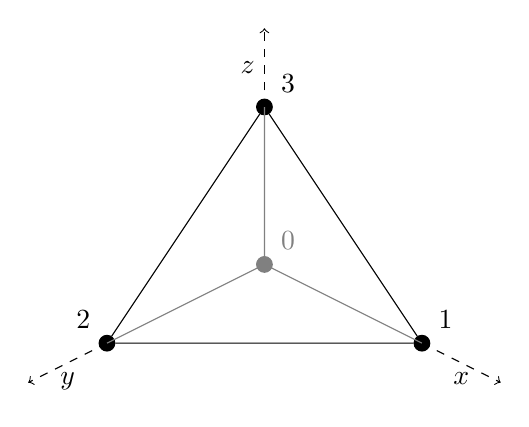
\begin{tikzpicture}
                        \node[inner sep=2pt, circle, draw=black!50, fill=black!50] at (0, 0) {};
                        \node[rbtb] (n3) at (0, 2) {};
                        \node[rbtb] (n1) at (2, -1) {};
                        \node[rbtb] (n2) at (-2, -1) {};

                        \node[black!50] at (0.3, 0.3) {0};
                        \node at (0.3, 2.3) {3};
                        \node at (2.3, -0.7) {1};
                        \node at (-2.3, -0.7) {2};

                        \draw[black!50]
                        (0, 0) -- (0, 2)
                        (0, 0) -- (2, -1)
                        (0, 0) -- (-2, -1);

                        \draw
                        (0, 2) edge[dashed, ->, left] node{$z$} (0, 3)
                        (2, -1) edge[dashed, ->, below] node{$x$} (3, -1.5)
                        (-2, -1) edge[dashed, ->, below] node{$y$} (-3, -1.5)
                        (n3) -- (n1) -- (n2) -- (n3);
                    \end{tikzpicture}
                \end{center}
                For this, we need a mixture of different data, including numerical data about the actual 3D coordinates of the vertices, as well as topological data regarding what vertices are connected to what.
                This can be represented in the following tables;
                \begin{center}
                    \hfill
                    \begin{tabular}{c|c}
                        \multicolumn{2}{c}{vertex data} \\
                        \hline
                        index & location \\
                        \hline
                        $0$ & $(0, 0, 0)$ \\
                        $1$ & $(1, 0, 0)$ \\
                        $2$ & $(0, 1, 0)$ \\
                        $3$ & $(0, 0, 1)$
                    \end{tabular}
                    \hfill
                    \begin{tabular}{c|c}
                        \multicolumn{2}{c}{face data} \\
                        \hline
                        index & vertices \\
                        \hline
                        $0$ & 0 1 3 \\
                        $1$ & 0 2 1 \\
                        $2$ & 0 3 2 \\
                        $3$ & 1 2 3
                    \end{tabular}
                    \hfill \phantom{}
                \end{center}
                This separation allows for the vertices to move without affecting the faces.
            \subsubsection*{Projections}
                In order to draw a 3D wire frame, the points must first be converted into a 2D representation, via a \textbf{projection}, which can then be drawn with simple drawing primitives.
                Intuitively, we have an observer (a focal point) where all viewing rays converge.
                The observer is located between a projection surface $P$ and an object $V$.
                While it's possible to project onto any surface, we only consider linear projections onto a flat surface.
            \subsubsection*{Orthographic Projections}
                The simplest form of a projection is an \textbf{orthographic projection}.
                The assumptions made are that the viewpoint is located at $z = -\infty$, and the plane of projection is $z = 0$.
                With the viewing point being infinitely far away, the rays become parallel.
                This gives all projectors the same direction;
                $$\vec{d} = \begin{bmatrix}
                    0 \\ 0 \\ -1
                \end{bmatrix}$$
                This gives the following, with each projection line having the equation $\vec{P} = \vec{V} + \mu \vec{d}$;
                \begin{center}
                    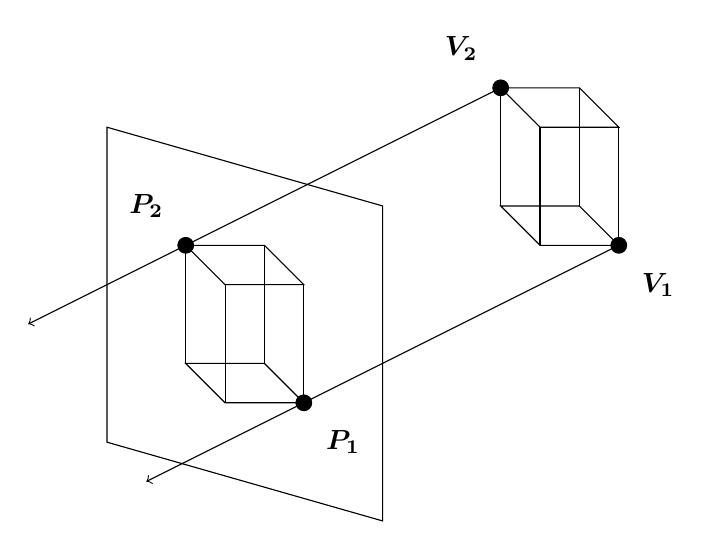
\begin{tikzpicture}
                        \draw (-1, 1.5) -- (2.5, 0.5) -- (2.5, -3.5) -- (-1, -2.5) -- cycle;
                        \begin{scope}[shift={(0, 0)}]
                            \draw (0, 0) -- (1, 0) -- (1.5, -0.5) -- (0.5, -0.5) -- cycle;
                            \draw (0, -1.5) -- (1, -1.5) -- (1.5, -2) -- (0.5, -2) -- cycle;
                            \draw
                            (0, 0) -- (0, -1.5)
                            (1, 0) -- (1, -1.5)
                            (1.5, -0.5) -- (1.5, -2)
                            (0.5, -0.5) -- (0.5, -2);
                        \end{scope}
                        \begin{scope}[shift={(4, 2)}]
                            \draw (0, 0) -- (1, 0) -- (1.5, -0.5) -- (0.5, -0.5) -- cycle;
                            \draw (0, -1.5) -- (1, -1.5) -- (1.5, -2) -- (0.5, -2) -- cycle;
                            \draw
                            (0, 0) -- (0, -1.5)
                            (1, 0) -- (1, -1.5)
                            (1.5, -0.5) -- (1.5, -2)
                            (0.5, -0.5) -- (0.5, -2);
                        \end{scope}

                        \draw
                        (4, 2) edge[->] (-2, -1)
                        (5.5, 0) edge[->] (-0.5, -3);

                        \node[rbtb] at (4, 2) {};
                        \node[rbtb] at (5.5, 0) {};
                        \node[rbtb] at (0, 0) {};
                        \node[rbtb] at (1.5, -2) {};

                        \node at (3.5, 2.5) {$\vec{V_2}$};
                        \node at (6, -0.5) {$\vec{V_1}$};
                        \node at (-0.5, 0.5) {$\vec{P_2}$};
                        \node at (2, -2.5) {$\vec{P_1}$};
                    \end{tikzpicture}
                \end{center}
                By substituting in the direction $\vec{d}$ we have determined, it gives the following Cartesian equations for each component;
                \begin{align*}
                    P_x & = V_x + 0 \\
                    P_y & = V_y + 0 \\
                    P_z & = V_z - \mu \\
                \end{align*}
                However, since we have the projection plane $z = 0$, we also know that $P_z = 0$, therefore we don't need to solve for $\mu$.
                From this, we can determine the projected location is the 3D $x$ and $y$ components of the vertex;
                $$\vec{P} = \begin{bmatrix}
                    V_x \\ V_y \\ 0
                \end{bmatrix}$$
                Viewing the wireframe for a cube directly from a face would look like the following;
                \begin{center}
                    \begin{tikzpicture}[x=1.5cm, y=1.5cm]
                        \draw (0, 0) -- (1, 0) -- (1, 1) -- (0, 1) -- cycle;
                    \end{tikzpicture}
                \end{center}
            \subsubsection*{Perspective Projection}
                While orthographic projections are fine when depth isn't a consideration (such as objects mostly being at the same distance from the viewer), it's insufficient for close work, where we want details to be realistic.
                The difference here is that we are no longer at an infinite distance (instead being at the origin), and the projection plane is $z = f$ (where $f$ stands for focal length);
                \begin{center}
                    \begin{tikzpicture}
                        \draw
                        (0, 0) edge[->] (10, 0)
                        (0, 0) edge[->] (0, 7);
                        \node at (-0.5, 7) {$y$};
                        \node at (10, -0.5) {$x$};
                        \node at (9, 4) {$z$};

                        \draw (2, 1) -- (2, 4) -- (6, 4) -- (6, 1) -- cycle;
                        \draw
                        (0, 0) -- (2, 1)
                        (2, 1) edge[dashed] (6, 3)
                        (6, 3) edge[->] (9, 4.5);

                        \draw (5, 7) -- (7, 6) -- (5.5, 5) -- cycle;
                        \node[rbtb] at (5, 7) {};
                        \node[rbtb] at (7, 6) {};
                        \node at (4.5, 7) {$\vec{V_1}$};
                        \node at (7.5, 6) {$\vec{V_2}$};

                        \draw (2.5, 3.5) -- (3.5, 3) -- (2.75, 2.5) -- cycle;
                        \node[rbtb] at (2.5, 3.5) {};
                        \node[rbtb] at (3.5, 3) {};
                        \node at (2, 3.5) {$\vec{P_1}$};
                        \node at (4, 3) {$\vec{P_2}$};

                        \draw[black!50]
                        (5, 7) -- (0, 0)
                        (7, 6) -- (0, 0);

                        \draw
                        (0, 0) edge[dashed] (0, -2)
                        (2, 1) edge[dashed] (2, -1)
                        (0, -1.5) edge[<->, below] node{$f$} (2, -0.5);
                    \end{tikzpicture}
                \end{center}
                This gives us the following equation (since all projectors must go through the origin);
                $$\vec{P} = \mu \vec{V}$$
                We can work out the value of $\mu$, let it be $\mu_p$ as follows;
                \begin{align*}
                    P_z & = f & \text{by projection plane} \\
                    \mu_p & = \frac{P_z}{V_z} \\
                    & = \frac{f}{V_z} \\
                    P_x & = \mu_p V_x \\
                    & = \frac{f V_x}{V_z} \\
                    P_y & = \mu_p V_y \\
                    & = \frac{f V_y}{V_z}
                \end{align*}
                Viewing the wireframe for a cube directly from a face would look like the following (note the difference to the orthographic projection);
                \begin{center}
                    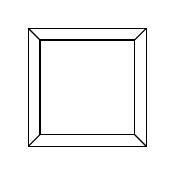
\begin{tikzpicture}[x=1.5cm, y=1.5cm]
                        \draw (0, 0) -- (1, 0) -- (1, 1) -- (0, 1) -- cycle;
                        \draw (0.1, 0.1) -- (0.9, 0.1) -- (0.9, 0.9) -- (0.1, 0.9) -- cycle;
                        \draw
                        (0, 0) -- (0.1, 0.1)
                        (1, 0) -- (0.9, 0.1)
                        (1, 1) -- (0.9, 0.9)
                        (0, 1) -- (0.1, 0.9);
                    \end{tikzpicture}
                \end{center}
            \subsubsection*{Transformations}
                Scenes are defined in a particular coordinate system, but we want to be able to draw a scene from any angle.
                To do so, it's easier to have the viewpoint at the origin, and the $z$-axis as the direction of view.
                As such, we need to be able to \textbf{transform} the coordinates of a scene.
                \begin{center}
                    \begin{tikzpicture}
                        \begin{scope}[shift={(0, 0)}]
                            \draw
                            (0, 0) edge[->, below] node{$x$} (5, 0)
                            (0, 0) edge[->, left] node{$y$} (0, 2)
                            (0, 0) edge[->, above] node{$z$} (2, 1);

                            \begin{scope}[shift={(2.5, 0.75)}]
                                \draw (0, 0) -- (1, 0) -- (1, 1) -- (0, 1) -- cycle;
                                \draw
                                (0, 0) -- (0.5, 0.5)
                                (1, 0) -- (1.5, 0.5)
                                (1, 1) -- (1.5, 1.5)
                                (0, 1) -- (0.5, 1.5);
                                \draw (0.5, 0.5) -- (1.5, 0.5) -- (1.5, 1.5) -- (0.5, 1.5) -- cycle;
                            \end{scope}

                            \draw
                            (0, 0) edge[dashed, ->, below] node{$C_x$} (4, 0)
                            (4, 0) edge[dashed, ->, right] node{\ \ $C_z$} (6, 1)
                            (6, 1) edge[dashed, ->, right] node{$C_y$} (6, 3)
                            (6, 3) edge[->, above] node{$\vec{d}$} (5, 2.5);

                            \node at (6.5, 3) {$\vec{C}$};
                            \node at (-0.5, 0) {$\vec{O}$};
                        \end{scope}
                        \begin{scope}[shift={(8, 0)}]
                            \draw
                            (0, 0) edge[dashed] (5, 0)
                            (0, 0) edge[dashed] (0, 2)
                            (0, 0) edge[dashed] (2, 1);

                            \begin{scope}[shift={(2.5, 0.75)}]
                                \draw (0, 0) -- (1, 0) -- (1, 1) -- (0, 1) -- cycle;
                                \draw
                                (0, 0) -- (0.5, 0.5)
                                (1, 0) -- (1.5, 0.5)
                                (1, 1) -- (1.5, 1.5)
                                (0, 1) -- (0.5, 1.5);
                                \draw (0.5, 0.5) -- (1.5, 0.5) -- (1.5, 1.5) -- (0.5, 1.5) -- cycle;
                            \end{scope}

                            \draw
                            (6, 3) edge[->, below] node{$z$} (5, 2.5)
                            (6, 3) edge[->, right] node{$y$} (5.5, 4)
                            (6, 3) edge[->, below] node{$x$} (5.25, 3.5);

                            \node at (6.5, 3) {$\vec{O}$};
                        \end{scope}
                    \end{tikzpicture}
                \end{center}
                These are done by the application of transformation matrices.
                For example, a standard transformation to make an object twice as big from the origin;
                $$\begin{bmatrix}
                    x^\prime \\ y^\prime \\ z^\prime
                \end{bmatrix} = \begin{bmatrix}
                    2 & 0 & 0 \\
                    0 & 2 & 0 \\
                    0 & 0 & 2
                \end{bmatrix} \begin{bmatrix}
                    x \\ y \\ z
                \end{bmatrix}$$
            \subsubsection*{Translation}
                However, being restricted to matrix operations with $\mathbb{R}^{3 \times 3}$ means that we cannot represent translations (for example, a shift of two units on the $x$-axis, such that $x^\prime = x + 2$).
                The solution to this is to use 4D \textbf{homogenous coordinates}, where we assume the fourth dimension is fixed to 1.
                $$\begin{bmatrix}
                    x^\prime \\ y^\prime \\ z^\prime \\ 1
                \end{bmatrix} = \begin{bmatrix}
                    1 & 0 & 0 & 2 \\
                    0 & 1 & 0 & 0 \\
                    0 & 0 & 1 & 0 \\
                    0 & 0 & 0 & 1
                \end{bmatrix} \begin{bmatrix}
                    x \\ y \\ z \\ 1
                \end{bmatrix}$$
                Frequently the last ordinate is 1, however in general it is a scale factor;
                $$\underbrace{(p_x, p_y, p_z, s)}_\text{homogenous} \Leftrightarrow \underbrace{\left(\frac{p_x}{s}, \frac{p_y}{s}, \frac{p_z}{s}\right)}_\text{Cartesian}$$
            \subsubsection*{Affine Transformations}
                Affine transformations preserve parallel lines.
                Most of the transformations we require are affine, with the most important being scaling, rotation, and translation;
                \begin{itemize}
                    \itemsep0em
                    \item \textbf{scaling} \hfill by $(s_x, s_y, s_z)$
                        $$\begin{bmatrix}
                            s_x & 0 & 0 & 1 \\
                            0 & s_y & 0 & 1 \\
                            0 & 0 & s_z & 1 \\
                            0 & 0 & 0 & 1
                        \end{bmatrix} \begin{bmatrix}
                            p_x \\ p_y \\ p_z \\ 1
                        \end{bmatrix} = \begin{bmatrix}
                            s_x p_x \\
                            s_y p_y \\
                            s_z p_z \\
                            1
                        \end{bmatrix}$$
                    \item \textbf{rotation}
                        \smallskip

                        In order to define a rotation, we need both an axis and an angle, with the simplest rotations being about the Cartesian axes.
                        The following matrices are used for rotations of $\theta$ about each of the axes;
                        \begin{align*}
                            \mat{\mathcal{R}_x} & = \begin{bmatrix}
                                1 & 0 & 0 & 0 \\
                                0 & \cos \theta & -\sin \theta & 0 \\
                                0 & \sin \theta & \cos \theta & 0 \\
                                0 & 0 & 0 & 1
                            \end{bmatrix} \\
                            \mat{\mathcal{R}_y} & = \begin{bmatrix}
                                \cos \theta & 0 & \sin \theta & 0 \\
                                0 & 1 & 0 & 0 \\
                                -\sin \theta & 0 & \cos \theta & 0 \\
                                0 & 0 & 0 & 1
                            \end{bmatrix} \\
                            \mat{\mathcal{R}_z} & = \begin{bmatrix}
                                \cos \theta & -\sin \theta & 0 & 0 \\
                                \sin \theta & \cos \theta & 0 & 0 \\
                                0 & 0 & 1 & 0 \\
                                0 & 0 & 0 & 1
                            \end{bmatrix}
                        \end{align*}
                        It's important to note that \textbf{rotations have a direction}.
                        In this course, we use a left-handed coordinate system, where the rotation is anti-clockwise when looking along the axis of rotation (think about the origin being closer to you, and the axis going off to $\infty$ away from you).
                    \item \textbf{translation} \hfill by $(t_x, t_y, t_z)$
                        $$\begin{bmatrix}
                            1 & 0 & 0 & t_x \\
                            0 & 1 & 0 & t_y \\
                            0 & 0 & 1 & t_z \\
                            0 & 0 & 0 & 1
                        \end{bmatrix} \begin{bmatrix}
                            p_x \\ p_y \\ p_z \\ 1
                        \end{bmatrix} = \begin{bmatrix}
                            p_x + t_x \\
                            p_y + t_y \\
                            p_z + t_z \\
                            1
                        \end{bmatrix}$$
                \end{itemize}
                However, perspective projections are an example of a non-affine transformation, as it doesn't preserve parallels.
                Intuitively, it's not invertible (singular), as we cannot convert from a photograph to a 3D model.
                \medskip

                Note that we should be careful when we combine transformation.
                As matrix multiplication isn't commutative, we should read a sequence of matrices multiplied together from right to left, with the right-most matrix, before the vector, being the \textbf{first} transformation to be applied.
        \subsection*{Lecture 2 - Transformations for Animation}
            Recall the transformation in the previous lecture, which took way too long to draw, moving the origin to the view point.
            It consists of three steps, with the latter two being used to align the $z$-axis with the view direction;
            \begin{enumerate}[1.]
                \itemsep0em
                \item translation of the origin \hfill fairly trivial to do
                    $$\mat{\mathcal{A}} = \begin{bmatrix}
                        1 & 0 & 0 & -C_x \\
                        0 & 1 & 0 & -C_y \\
                        0 & 0 & 1 & -C_z \\
                        0 & 0 & 0 & 1
                    \end{bmatrix}$$
                \item rotation about $y$-axis
                    \smallskip

                    Consider the following, looking at the $x-z$ plane;
                    \begin{center}
                        \begin{tikzpicture}[x=0.75cm, y=0.75cm]
                            \draw
                            (0, 0) edge[->] (0, 6)
                            (0, 0) edge[->] (6, 0)
                            (0, 0) edge[very thick, ->] (3, 4)
                            (0, 0) edge[very thick, ->] (0, 5)
                            (0, 0) edge[dashed, <->, below] node{$d_x$} (3, 0)
                            (3, 0) edge[dashed, <->, right] node{$d_z$} (3, 4);

                            \draw (0, 0) ++(53:1) arc (53:90:1);
                            \node at (0.4, 1.25) {$\theta$};

                            \node at (2.5, 4) {$\vec{v}$};
                            \node at (6, -0.5) {$x$};
                            \node at (-0.5, 6) {$z$};
                        \end{tikzpicture}
                    \end{center}
                    This can be used to calculate the following (note that here we are using a right-handed system);
                    \begin{align*}
                        || \vec{v} || & = v \\
                        & = \sqrt{d_x^2 + d_z^2} \\
                        \cos \theta & = \frac{d_z}{v} \\
                        \sin \theta & = \frac{d_x}{v} \\
                        \mat{\mathcal{B}} & = \begin{bmatrix}
                            \cos \theta & 0 & -\sin \theta & 0 \\
                            0 & 1 & 0 & 0 \\
                            -\sin \theta & 0 & \cos \theta & 0 \\
                            0 & 0 & 0 & 1
                        \end{bmatrix} \\
                        & = \begin{bmatrix}
                            \frac{d_z}{v} & 0 & -\frac{d_x}{v} & 0 \\
                            0 & 1 & 0 & 0 \\
                            \frac{d_x}{v} & 0 & \frac{d_z}{v} & 0 \\
                            0 & 0 & 0 & 1
                        \end{bmatrix}
                    \end{align*}
                \item rotation about $x$-axis
                    \smallskip

                    This follows a similar process, note that we are now aligned along the $y-z$ plane (for clarity, the horizontal distance is $v$);
                    \begin{center}
                        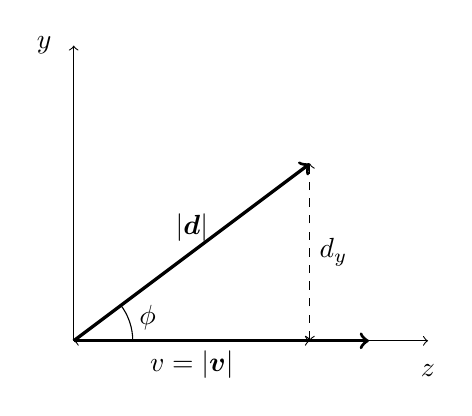
\begin{tikzpicture}[x=0.75cm, y=0.75cm]
                            \draw
                            (0, 0) edge[->] (6, 0)
                            (0, 0) edge[->] (0, 5)
                            (0, 0) edge[very thick, ->, above] node{$| \vec{d} |$} (4, 3)
                            (0, 0) edge[very thick, ->] (5, 0)
                            (0, 0) edge[dashed, <->, below] node{$v = | \vec{v} |$} (4, 0)
                            (4, 0) edge[dashed, <->, right] node{$d_y$} (4, 3);

                            \draw (0, 0) ++(38:1) arc (38:0:1);
                            \node at (1.25, 0.4) {$\phi$};
                            \node at (6, -0.5) {$z$};
                            \node at (-0.5, 5) {$y$};
                        \end{tikzpicture}
                    \end{center}
                    Similarly, the matrix can be obtained as follows;
                    \begin{align*}
                        \cos \phi & = \frac{v}{| \vec{d} |} \\
                        \sin \phi & = \frac{d_y}{| \vec{d} |} \\
                        \mat{\mathcal{C}} & = \begin{bmatrix}
                            1 & 0 & 0 & 0 \\
                            0 & \cos \phi & -\sin \phi & 0 \\
                            0 & \sin \phi & \cos \phi & 0 \\
                            0 & 0 & 0 & 1
                        \end{bmatrix} \\
                        & = \begin{bmatrix}
                            1 & 0 & 0 & 0 \\
                            0 & \frac{v}{| \vec{d} |} & -\frac{d_y}{| \vec{d} |} & 0 \\
                            0 & \frac{d_y}{| \vec{d} |} & \frac{v}{| \vec{d} |} & 0 \\
                            0 & 0 & 0 & 1
                        \end{bmatrix}
                    \end{align*}
            \end{enumerate}
            From this, we are able to combine the matrices into the following;
            $$\mat{\mathcal{T}} = \mat{\mathcal{C}} \mat{\mathcal{B}} \mat{\mathcal{A}}$$
            For every point $\vec{P}$ in the scene, we can obtain $\vec{P_t} = \mat{\mathcal{T}}\vec{P}$, with the view in \textbf{canonical} form, allowing us to apply the standard perspective or orthographic projection.
            \subsubsection*{Rotation About a General Line}
                Rotation of a scene around a general line can be done as a combination of transformations.
                The idea is similar, with the following three steps;
                \begin{enumerate}[1.]
                    \itemsep0em
                    \item making the line of rotation one of the Cartesian axes
                        \smallskip

                        This uses the matrices derived before, rotating the general line to be aligned with the $z$-axis.
                    \item perform the rotation
                        \smallskip

                        Standard rotation around the $z$-axis defined previously.
                    \item restore line to original place
                        \smallskip

                        Inversion of the initial matrices to revert rotation.
                \end{enumerate}
                This gives us the following full matrix;
                $$\mat{\mathcal{T}} = \underbrace{\mat{\mathcal{A}^{-1}} \mat{\mathcal{B}^{-1}} \mat{\mathcal{C}^{-1}}}_3 \underbrace{\mat{\mathcal{R}_z}}_2 \underbrace{\mat{\mathcal{C}} \mat{\mathcal{B}} \mat{\mathcal{A}}}_1$$
            \subsubsection*{Projection Matrices}
                For the canonical / orthographic projection, the matrix simply drops the $z$ component;
                \begin{align*}
                    \mat{\mathcal{M}_O} & = \begin{bmatrix}
                        1 & 0 & 0 & 0 \\
                        0 & 1 & 0 & 0 \\
                        0 & 0 & 0 & 0 \\
                        0 & 0 & 0 & 1
                    \end{bmatrix} \\
                    \mat{\mathcal{M}_O} \begin{bmatrix}
                        x \\ y \\ z \\ 1
                    \end{bmatrix} & = \begin{bmatrix}
                        x \\ y \\ 0 \\ 1
                    \end{bmatrix}
                \end{align*}
                This is clearly non-invertible, as we are losing information about one of the axes.
                An effect of this is that we must do any effects in 3D \textbf{before} applying the projection matrix.
                \medskip

                The perspective projection matrix can also be done in a similar way;
                \begin{align*}
                    \mat{\mathcal{M}_p} & = \begin{bmatrix}
                        1 & 0 & 0 & 0 \\
                        0 & 1 & 0 & 0 \\
                        0 & 0 & 1 & 0 \\
                        0 & 0 & \frac{1}{f} & 0
                    \end{bmatrix} \\
                    \mat{\mathcal{M}_p} \begin{bmatrix}
                        x \\ y \\ z \\ 1
                    \end{bmatrix} & = \begin{bmatrix}
                        x \\ y \\ z \\ \frac{z}{f}
                    \end{bmatrix} \\
                    & \rightarrow \begin{bmatrix}
                        \frac{fx}{z} \\
                        \frac{fy}{z} \\
                        f \\
                        1
                    \end{bmatrix} & \text{using the fourth ordinate as a scale factor}
                \end{align*}
                Note that homogenous coordinates and vectors fall into one of two types;
                \begin{enumerate}[1.]
                    \itemsep0em
                    \item \textbf{position vectors}
                        \smallskip

                        These have a non-zero final ordinate ($s > 0$) and can be normalised to Cartesian form.
                        If two position vectors are added, we instead obtain the mid-point;
                        $$\begin{bmatrix}
                            X_a \\ Y_a \\ Z_a \\ 1
                        \end{bmatrix} + \begin{bmatrix}
                            X_b \\ Y_b \\ Z_b \\ 1
                        \end{bmatrix} = \begin{bmatrix}
                            X_a + X_b \\
                            Y_a + Y_b \\
                            Z_a + Z_b \\
                            2
                        \end{bmatrix} = \begin{bmatrix}
                            \frac{X_a + X_b}{2} \\
                            \frac{Y_a + Y_b}{2} \\
                            \frac{Z_a + Z_b}{2} \\
                            1
                        \end{bmatrix}$$
                        This has no real meaning in geometry, but is a useful observation.
                    \item \textbf{direction vectors}
                        \smallskip

                        These have a zero in the final ordinate, and have a direction and magnitude.
                        If two direction vectors are added, we obtain a direction vector (following the normal addition rule);
                        $$\begin{bmatrix}
                            x_i \\ y_i \\ z_i \\ 0
                        \end{bmatrix} + \begin{bmatrix}
                            x_j \\ y_j \\ z_j \\ 0
                        \end{bmatrix} = \begin{bmatrix}
                            x_i + x_j \\
                            y_i + y_j \\
                            z_i + z_j \\
                            0
                        \end{bmatrix}$$
                        However, if a direction vector is added to a position vector, we obtain another position vector;
                        $$\begin{bmatrix}
                            X \\ Y \\ Z \\ 1
                        \end{bmatrix} + \begin{bmatrix}
                            x \\ y \\ z \\ 0
                        \end{bmatrix} = \begin{bmatrix}
                            X + x \\
                            Y + y \\
                            Z + z \\
                            1
                        \end{bmatrix}$$
                \end{enumerate}
            \subsubsection*{Structure of a Transformation Matrix}
                Note that the bottom row of such a matrix is \textbf{always} 0 0 0 1.
                We can decompose the columns of a transformation matrix into three direction vectors and one position vector.
                The three direction vectors are the new axes and the position vector is the new origin.
                $$\underbrace{\begin{bmatrix}
                    q_x & r_x & s_x & C_x \\
                    q_y & r_y & s_y & C_y \\
                    q_z & r_z & s_z & C_z \\
                    0 & 0 & 0 & 1
                \end{bmatrix}}_\text{matrix} \rightarrow \underbrace{\begin{bmatrix}
                    q_x \\ q_y \\ q_z \\ 0
                \end{bmatrix} \begin{bmatrix}
                    r_x \\ r_y \\ r_z \\ 0
                \end{bmatrix} \begin{bmatrix}
                    s_x \\ s_y \\ s_z \\ 0
                \end{bmatrix}}_\text{direction vectors} \underbrace{\begin{bmatrix}
                    C_x \\ C_y \\ C_z \\ 1
                \end{bmatrix}}_\text{position vector}$$
                When applying this transformation to a direction vector, where the last ordinate is zero, no \textbf{translation} is applied.
                On the other hand, if it is a position vector, where the last ordinate is 1, all vectors will have the same displacement.
                \medskip

                The following results can be proved by observing changes to the standard basis vectors, and the origin after applying the matrix;
                \begin{itemize}
                    \itemsep0em
                    \item $\vec{q}$ \hfill transformed $x$-axis
                    \item $\vec{r}$ \hfill transformed $y$-axis
                    \item $\vec{s}$ \hfill transformed $z$-axis
                    \item $\vec{C}$ \hfill transformed origin
                \end{itemize}
            \subsubsection*{Dot Product}
                We can consider the dot product as a projection;
                $$\vec{P} \cdot \vec{u} = | \vec{P} | | \vec{u} | \cos \theta$$
                Visually, we can see the dot product as the following;
                \begin{center}
                    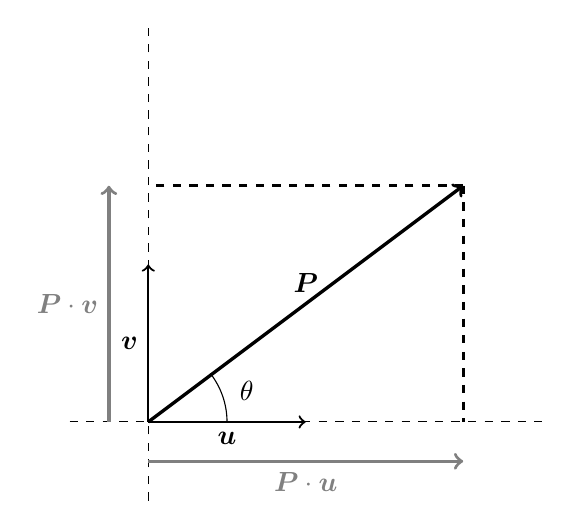
\begin{tikzpicture}
                        \draw
                        (-1, 0) edge[dashed] (5, 0)
                        (0, -1) edge[dashed] (0, 5)
                        (0, 0) edge[thick, ->, below] node{$\vec{u}$} (2, 0)
                        (0, 0) edge[thick, ->, left] node{$\vec{v}$} (0, 2)
                        (0, 0) edge[very thick, ->, above] node{$\vec{P}$} (4, 3)
                        (4, 3) edge[very thick, dashed] (0, 3)
                        (4, 3) edge[very thick, dashed] (4, 0);
                        \draw (0, 0) ++(38:1) arc (38:0:1);
                        \node at (1.25, 0.4) {$\theta$};
                        \draw[black!50]
                        (0, -0.5) edge[very thick, ->, below] node{$\vec{P} \cdot \vec{u}$} (4, -0.5)
                        (-0.5, 0) edge[very thick, ->, left] node{$\vec{P} \cdot \vec{v}$} (-0.5, 3);
                    \end{tikzpicture}
                \end{center}
                If $\vec{u}$ is along a co-ordinate axis, then $\vec{P} \cdot \vec{u}$ is the ordinate of $\vec{P}$ in the direction of $\vec{u}$.
                \medskip

                Consider changing to the new axes $\vec{u}, \vec{v}, \vec{w}$, and origin $\vec{C}$.
                We can call the first co-ordinate of $\vec{P}$ in the new system $\vec{P}_x^t$;
                \begin{align*}
                    \vec{P}_x^t & = (\vec{P} - \vec{C}) \cdot \vec{u} \\
                    & = \vec{P} \cdot \vec{u} - \vec{C} \cdot \vec{u}
                \end{align*}
                However, this can also be represented in matrix notation;
                $$\begin{bmatrix}
                    P_x^t \\
                    P_y^t \\
                    P_z^t \\
                    1
                \end{bmatrix} = \begin{bmatrix}
                    u_x & u_y & u_z & -\vec{C} \cdot \vec{u} \\
                    v_x & v_y & v_z & -\vec{C} \cdot \vec{v} \\
                    w_x & w_y & w_z & -\vec{C} \cdot \vec{w} \\
                    0 & 0 & 0 & 1
                \end{bmatrix} \begin{bmatrix}
                    P_x \\
                    P_y \\
                    P_z \\
                    1
                \end{bmatrix}$$
                Returning to the original problem, where we need to find a transformation matrix with a viewpoint $\vec{C}$ and direction $\vec{d}$.
                This can be done by first finding the vectors $\vec{u}, \vec{v}, \vec{w}$.
                Since $\vec{d}$ is the direction of the new axes, we can write (to get a unit vector);
                $$\vec{w} = \frac{\vec{d}}{| \vec{d} |}$$
                We also want to maintain an orthogonal basis, as well as all unit vectors.
                For the horizontal direction, we can write $\vec{u}$ in terms of some horizontal vector $\vec{p}$;
                \begin{align*}
                    \vec{u} & = \frac{\vec{p}}{| \vec{p} |} \\
                    p_y & = 0 & \text{ensure horizontal, no vertical component}
                \end{align*}
                Similarly, we want some vertical vector $\vec{q}$ to write $\vec{v}$;
                \begin{align*}
                    \vec{v} & = \frac{\vec{q}}{| \vec{q} |} \\
                    q_y & = 1 & \text{vertical, positive component}
                \end{align*}
                This gives us the following to solve;
                \begin{align*}
                    \vec{p} & = \begin{bmatrix}
                        p_x \\ 0 \\ p_z
                    \end{bmatrix} & \text{new horizontal} \\
                    \vec{q} & = \begin{bmatrix}
                        q_x \\ 1 \\ q_z
                    \end{bmatrix} & \text{new vertical}
                \end{align*}
                However, the view direction can also be written as the following (since we have the view direction, which happens to be the new $z$-axis as perpendicular to the remaining two vectors);
                $$\vec{d} = \vec{p} \times \vec{q}$$
                Using this, we can write $\vec{p}$ in terms of $\vec{q}$;
                \begin{align*}
                    \vec{d} & = \begin{bmatrix}
                        d_x \\ d_y \\ d_z
                    \end{bmatrix} \\
                    & = \vec{p} \times \vec{q} \\
                    & = \begin{vmatrix}
                        \vec{i} & \vec{j} & \vec{k} \\
                        p_x & 0 & p_z \\
                        q_x & 1 & q_z
                    \end{vmatrix} \\
                    & = -p_z \vec{i} + (p_z q_x - p_x q_z) \vec{j} + p_x \vec{k} \\
                    & = \begin{bmatrix}
                        -p_z \\
                        p_z q_x - p_x q_z \\
                        p_x
                    \end{bmatrix} & \Rightarrow \\
                    d_x & = -p_z \\
                    d_y & = p_z q_x - p_x q_z \\
                    d_z & = p_x & \Rightarrow \\
                    \vec{p} & = \begin{bmatrix}
                        d_z \\ 0 \\ -d_x
                    \end{bmatrix}
                \end{align*}
                However, since we know that the vectors $\vec{p}$ and $\vec{q}$ are orthogonal, we can say the following;
                \begin{align*}
                    \vec{p} \cdot \vec{q} & = 0 & \Rightarrow \\
                    p_x q_x + p_z q_z & = 0 \\
                    d_y & = p_z q_x - p_x q_z & \text{from above}
                \end{align*}
                Both of these equations can be fully written in terms of $\vec{d}$.
        \subsection*{Lecture 3 - Clipping and 3D Geometry}
            \textbf{Clipping} is the process of eliminating portions of objects outside the \textbf{viewing frustum} (boundaries of the image plane projected in 3D, consisting of a near and far clipping plane).
            This is useful to avoid degeneracy (by not drawing objects behind the camera), as well as improving efficiency by not processing objects which won't be visible.
            \medskip

            There are three points when we could clip;
            \begin{itemize}
                \itemsep0em
                \item before perspective transform (3D space) \hfill world co-ordinates
                \item after perspective transform \hfill homogeneous co-ordinates
                \item after perspective division \hfill screen space
            \end{itemize}
            The second option, in camera co-ordinates, is ideal.
            This is because the clipping planes are axis aligned, as we can discard anything further than the far plane or closer than the near plane.
            \subsubsection*{Halfspace}
                We can define any infinite line (for simplicity, in 2D) as a test;
                $$f(x, y) = 0 \text{ such as } \violet{x - y + 1 = 0}$$
                \begin{center}
                    \begin{tikzpicture}
                        \draw
                        (0, -1) edge[->] (0, 4)
                        (-2, 0) edge[->] (4, 0);
                        \node at (-0.5, 4) {$y$};
                        \node at (4, -0.5) {$x$};

                        \node at (2, 1) {\shortstack{halfspace\\$f(x, y) > 0$}};
                        \node at (-2, 2) {\shortstack{halfspace\\$f(x, y) < 0$}};

                        \draw[violet] (-2, -1) -- (3, 4);
                    \end{tikzpicture}
                \end{center}
                In 3D, the plane equation is $f(x, y, z) = Ax + By + Cz + D = 0$, which also divides space into two spaces, one where the test is positive, and one where it is negative.
                \medskip

                Note that we can define $\vec{H}$ as the normal vector of our plane, and also normalise it to avoid infinite solutions by scaling;
                \begin{align*}
                    \vec{H} & = \begin{bmatrix}
                        A \\ B \\ C \\ D
                    \end{bmatrix} \\
                    A^2 + B^2 + C^2 & = 1
                \end{align*}
                The distance is quite easily calculated as follows;
                $$d = \vec{H} \cdot \vec{P} = \vec{H}^\top\vec{P}$$
                This is a \textbf{signed} distance, where a positive value would denote inside, and a negative value would denote outside.
                \medskip

                Consider the \textbf{view frustum}, where we have 6 planes, and their normals oriented towards the interior of the frustum (where each plane has its own $\vec{H}$).
                If $\vec{H} \cdot \vec{P} < 0$ for \textbf{any} of the planes, then it is clipped, as it would be outside of the frustum.
        \subsection*{Lecture 4 - Graphics Pipelines and APIs}
            All graphics systems work according to some fundamental principles, we can define two conceptually related graphics pipelines;
            \begin{itemize}
                \itemsep0em
                \item \textbf{declarative} \hfill tell system what we want to render, not how
                    \smallskip

                    Relates to OOP.
                    For example, we can define a sphere which knows about its environment, and its location etc, and can draw itself with graphics primitives (essentially how to tessellate itself).
                    Virtual cameras, and scene descriptions (scene graphs) can also exist.
                    Every object may know about each other.
                \item \textbf{imperative} \hfill tell the system how to render something, but not what is being rendered
                    \smallskip

                    In contrast, the pipeline here now takes in a sequence of drawing commands, such as drawing a vertex at a given position.
                    As such, objects can be drawn independent from each other, allowing for a degree of parallelism.
            \end{itemize}
            It's important to note that we build declarative pipelines on top of an imperative model.
            For example, the sphere should know how to tessellate itself, and send the commands to the imperative backend.
            \begin{center}
                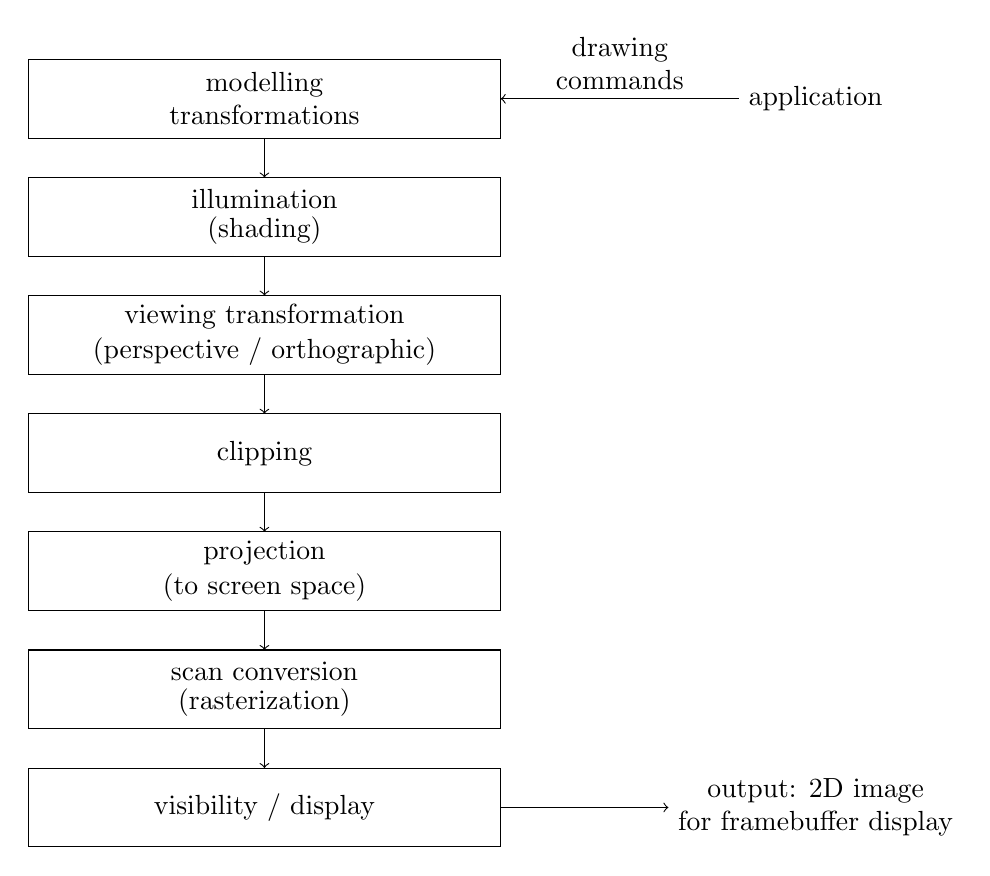
\begin{tikzpicture}[y=-1cm]
                    \begin{scope}[shift={(0, 0)}]
                        \draw (0, 0) -- (6, 0) -- (6, 1) -- (0, 1) -- cycle;
                        \node at (3, 0.5) {\shortstack{modelling\\transformations}};
                    \end{scope}
                    \begin{scope}[shift={(0, 1.5)}]
                        \draw (0, 0) -- (6, 0) -- (6, 1) -- (0, 1) -- cycle;
                        \node at (3, 0.5) {\shortstack{illumination\\(shading)}};
                    \end{scope}
                    \begin{scope}[shift={(0, 3)}]
                        \draw (0, 0) -- (6, 0) -- (6, 1) -- (0, 1) -- cycle;
                        \node at (3, 0.5) {\shortstack{viewing transformation\\(perspective / orthographic)}};
                    \end{scope}
                    \begin{scope}[shift={(0, 4.5)}]
                        \draw (0, 0) -- (6, 0) -- (6, 1) -- (0, 1) -- cycle;
                        \node at (3, 0.5) {\shortstack{clipping}};
                    \end{scope}
                    \begin{scope}[shift={(0, 6)}]
                        \draw (0, 0) -- (6, 0) -- (6, 1) -- (0, 1) -- cycle;
                        \node at (3, 0.5) {\shortstack{projection\\(to screen space)}};
                    \end{scope}
                    \begin{scope}[shift={(0, 7.5)}]
                        \draw (0, 0) -- (6, 0) -- (6, 1) -- (0, 1) -- cycle;
                        \node at (3, 0.5) {\shortstack{scan conversion\\(rasterization)}};
                    \end{scope}
                    \begin{scope}[shift={(0, 9)}]
                        \draw (0, 0) -- (6, 0) -- (6, 1) -- (0, 1) -- cycle;
                        \node at (3, 0.5) {\shortstack{visibility / display}};
                    \end{scope}
                    \node (a) at (10, 0.5) {application};
                    \node (o) at (10, 9.5) {\shortstack{output: 2D image\\for framebuffer display}};
                    \draw
                    (3, 1) edge[->] (3, 1.5)
                    (3, 2.5) edge[->] (3, 3)
                    (3, 4) edge[->] (3, 4.5)
                    (3, 5.5) edge[->] (3, 6)
                    (3, 7) edge[->] (3, 7.5)
                    (3, 8.5) edge[->] (3, 9)
                    (a) edge[->, above] node{\shortstack{drawing\\commands}} (6, 0.5)
                    (6, 9.5) edge[->] (o);
                \end{tikzpicture}
            \end{center}
            The steps of the pipeline perform the following;
            \begin{itemize}
                \itemsep0em
                \item \textbf{modelling transformations}
                    \smallskip

                    As 3D models are defined in the own coordinate systems (might all be at the origin, etc.), modelling transformations orients the models within the world coordinates (as a common coordinate frame).
                    This can include scaling, rotation, and transformations.
                \item \textbf{illumination (shading)}
                    \smallskip

                    Approximate lighting model to give initial ideas for how the object may be illuminated.
                    The main illumination is done at this step, before clipping, in order to get accurate shadows (which may have been clipped).
                \item \textbf{viewing transformation}
                    \smallskip

                    The world space is mapped into camera space.
                    The viewing position is transformed to the origin, and the viewing direction is oriented along the $z$ axis (typically).
                \item \textbf{clipping}
                    \smallskip

                    Remove portions of the scene outside the view frustum.
                    Transformation is also performed to Normalised Device Coordinates (pictured below).
                    \begin{center}
                        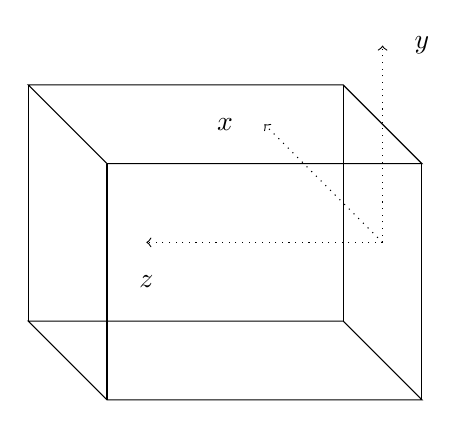
\begin{tikzpicture}
                            \draw (0, 0) -- (4, 0) -- (5, -1) -- (1, -1) -- cycle;
                            \draw (0, -3) -- (4, -3) -- (5, -4) -- (1, -4) -- cycle;
                            \draw
                            (0, 0) -- (0, -3)
                            (4, 0) -- (4, -3)
                            (5, -1) -- (5, -4)
                            (1, -1) -- (1, -4);
                            \draw
                            (4.5, -2) edge[dotted, ->] (4.5, 0.5)
                            (4.5, -2) edge[dotted, ->] (1.5, -2)
                            (4.5, -2) edge[dotted, ->] (3, -0.5);
                            \node at (5, 0.5) {$y$};
                            \node at (2.5, -0.5) {$x$};
                            \node at (1.5, -2.5) {$z$};
                        \end{tikzpicture}
                    \end{center}
                \item \textbf{projection}
                    \smallskip

                    The objects are projected into the 2D imaging plane screen space (see below);
                    \begin{center}
                        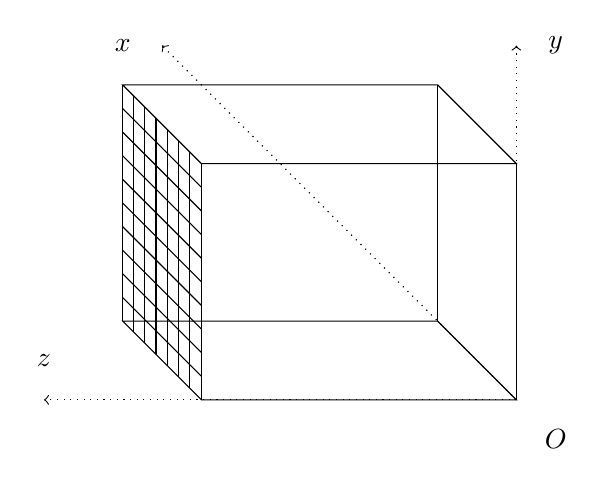
\begin{tikzpicture}
                            \draw (0, 0) -- (4, 0) -- (5, -1) -- (1, -1) -- cycle;
                            \draw (0, -3) -- (4, -3) -- (5, -4) -- (1, -4) -- cycle;
                            \draw
                            (0, 0) -- (0, -3)
                            (4, 0) -- (4, -3)
                            (5, -1) -- (5, -4)
                            (1, -1) -- (1, -4);
                            \draw
                            (5, -4) edge[dotted, ->] (5, 0.5)
                            (5, -4) edge[dotted, ->] (0.5, 0.5)
                            (5, -4) edge[dotted, ->] (-1, -4);
                            \node at (5.5, 0.5) {$y$};
                            \node at (0, 0.5) {$x$};
                            \node at (-1, -3.5) {$z$};
                            \node at (5.5, -4.5) {$O$};
                            \foreach \y in {0,...,8} {
                                \draw (0, -0.3 * \y - 0.3) -- (1, -0.3 * \y - 1.3);
                            }
                            \foreach \x in {0,...,5} {
                                \draw (0.1412 * \x + 0.1412, -0.1412 * \x - 3.1412) -- (0.1412 * \x + 0.1412, -0.1412 * \x - 0.1412);
                            }
                        \end{tikzpicture}
                    \end{center}
                \item \textbf{rasterization}
                    \smallskip

                    Converts objects into pixels, and interpolates values inside objects.
                    Due to hardware support, it's more efficient to just rasterize everything.
                \item \textbf{visibility / display}
                    \smallskip

                    Handles occlusions and transparency blending, as well as determining which objects are closest (and hence visible).
            \end{itemize}
            The majority of real-time graphics is based on the rasterization of graphic primitives (points, lines, triangles, etc).
            This is typically implemented in hardware (GPU), and is controlled through an API such as OpenGL.
            Certain parts of the pipeline are programmable, such as with GLSL (shaders).
            \medskip

            A \textbf{vertex} is a point in space defining geometry and a \textbf{fragment} is a sample produced during rasterization (multiple of which are merged into pixels).
            The high level view of the pipeline is as follows;
            \begin{center}
                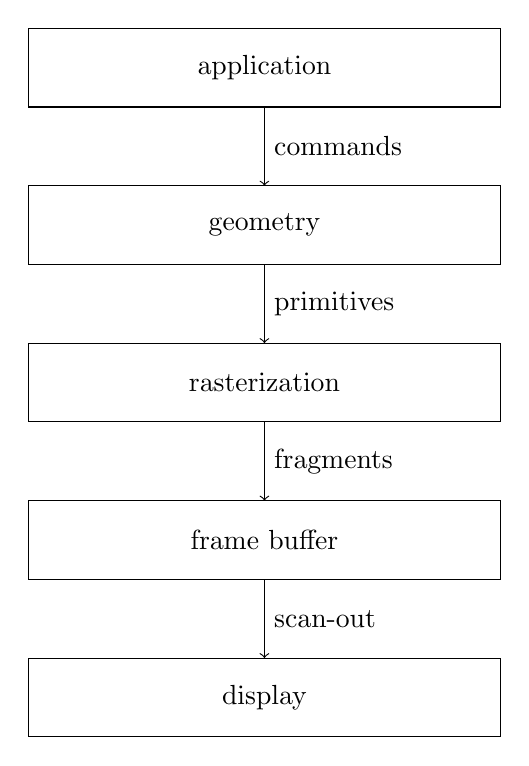
\begin{tikzpicture}[y=-1cm]
                    \begin{scope}[shift={(0, 0)}]
                        \draw (0, 0) -- (6, 0) -- (6, 1) -- (0, 1) -- cycle;
                        \node at (3, 0.5) {application};
                    \end{scope}
                    \begin{scope}[shift={(0, 2)}]
                        \draw (0, 0) -- (6, 0) -- (6, 1) -- (0, 1) -- cycle;
                        \node at (3, 0.5) {geometry};
                    \end{scope}
                    \begin{scope}[shift={(0, 4)}]
                        \draw (0, 0) -- (6, 0) -- (6, 1) -- (0, 1) -- cycle;
                        \node at (3, 0.5) {rasterization};
                    \end{scope}
                    \begin{scope}[shift={(0, 6)}]
                        \draw (0, 0) -- (6, 0) -- (6, 1) -- (0, 1) -- cycle;
                        \node at (3, 0.5) {frame buffer};
                    \end{scope}
                    \begin{scope}[shift={(0, 8)}]
                        \draw (0, 0) -- (6, 0) -- (6, 1) -- (0, 1) -- cycle;
                        \node at (3, 0.5) {display};
                    \end{scope}
                    \draw
                    (3, 1) edge[->, right] node{commands} (3, 2)
                    (3, 3) edge[->, right] node{primitives} (3, 4)
                    (3, 5) edge[->, right] node{fragments} (3, 6)
                    (3, 7) edge[->, right] node{scan-out} (3, 8);
                \end{tikzpicture}
            \end{center}
            It's important to draw a distinction in which stage we're working.
            When we have geometry processing and write shaders to do something with our vertices, we are at a vertex stage (everything lives in 3D coordinates).
            \subsubsection*{Application Stage}
                At the application stage, we typically generate a database of the scene (loaded from disks), and perform simulations (physics).
                Input events are also handled here.
                In this stage, objects are just vertex coordinates, and how they are connected.
                \medskip

                The lecture now goes over the graphics pipeline in \textbf{OpenGL 3.2}.
                It's important to note that many fixed functions (including tessellation primitive generation, rasterization and interpolation) are implemented in hardware, for performance.
            \subsubsection*{Geometry Stage}
                \begin{center}
                    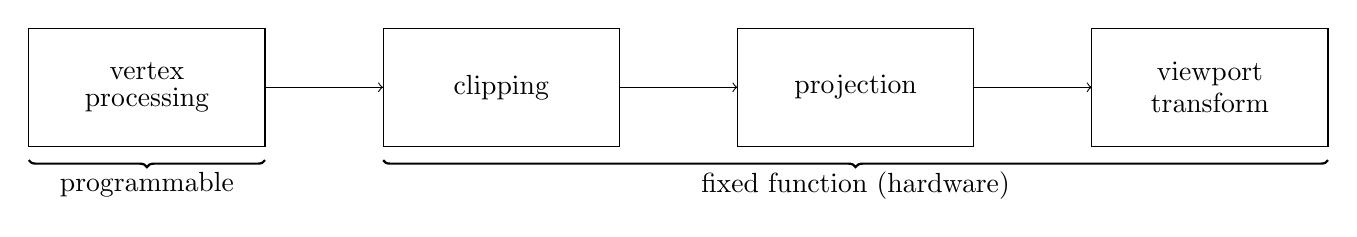
\begin{tikzpicture}[x=0.75cm, y=0.75cm]
                        \draw (0, 0) -- (4, 0) -- (4, -2) -- (0, -2) -- cycle;
                        \draw (6, 0) -- (10, 0) -- (10, -2) -- (6, -2) -- cycle;
                        \draw (12, 0) -- (16, 0) -- (16, -2) -- (12, -2) -- cycle;
                        \draw (18, 0) -- (22, 0) -- (22, -2) -- (18, -2) -- cycle;
                        \node at (2, -1) {\shortstack{vertex\\processing}};
                        \node at (8, -1) {\shortstack{clipping}};
                        \node at (14, -1) {\shortstack{projection}};
                        \node at (20, -1) {\shortstack{viewport\\transform}};
                        \draw[
                            thick,
                            decoration={
                                brace,
                                mirror,
                                raise=5
                            },
                            decorate
                        ] (0, -2) -- (4, -2) node[pos=0.5, anchor=north, yshift=-5.55] {programmable};
                        \draw[
                            thick,
                            decoration={
                                brace,
                                mirror,
                                raise=5
                            },
                            decorate
                        ] (6, -2) -- (22, -2) node[pos=0.5, anchor=north, yshift=-5.55] {fixed function (hardware)};
                        \draw
                        (4, -1) edge[->] (6, -1)
                        (10, -1) edge[->] (12, -1)
                        (16, -1) edge[->] (18, -1);
                    \end{tikzpicture}
                \end{center}
                In the vertex processing stage, the input vertex stream (composed of arbitrary vertex attributes such as position and colour) is transformed into a stream of vertices mapped onto the screen by the vertex shader.
                The following is the vertex post-processing pipeline (we can pre-multiply matrices if we don't need to do anything between the stages - typically we want to do stuff before the \textbf{projection matrix} however);
                \begin{center}
                    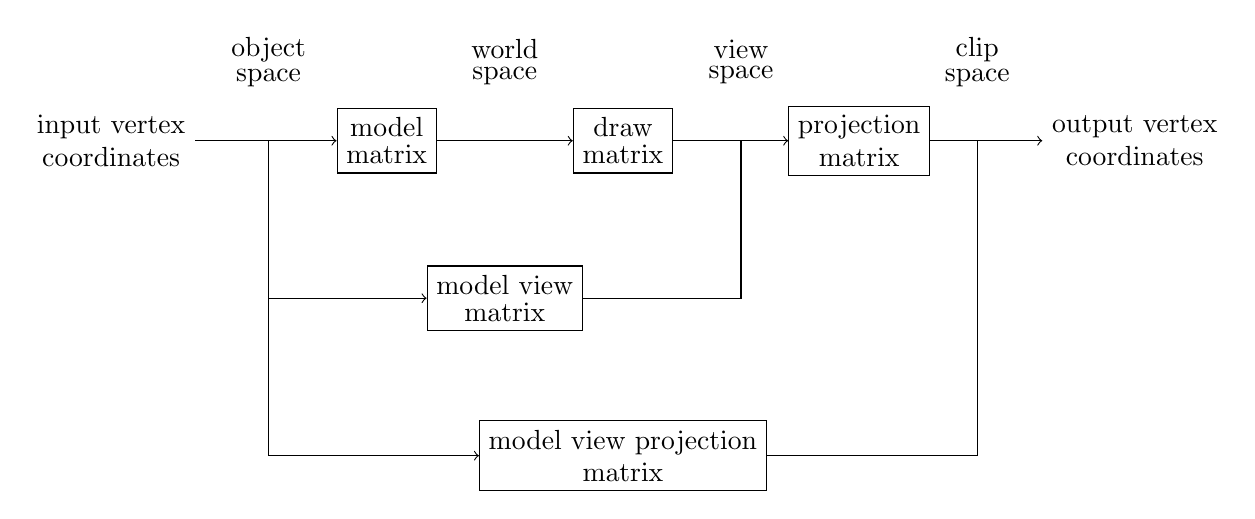
\begin{tikzpicture}
                        \node (ivc) at (-0.5, 0) {\shortstack{input vertex\\coordinates}};
                        \node[draw] (mm) at (3, 0) {\shortstack{model\\matrix}};
                        \node[draw] (dm) at (6, 0) {\shortstack{draw\\matrix}};
                        \node[draw] (pm) at (9, 0) {\shortstack{projection\\matrix}};
                        \node (ovc) at (12.5, 0) {\shortstack{output vertex\\coordinates}};
                        \node[draw] (mvm) at (4.5, -2) {\shortstack{model view\\matrix}};
                        \node[draw] (mvpm) at (6, -4) {\shortstack{model view projection\\matrix}};
                        \draw
                        (ivc) edge[->] (mm)
                        (mm) edge[->] (dm)
                        (dm) edge[->] (pm)
                        (pm) edge[->] (ovc)
                        (1.5, 0) -- (1.5, -4)
                        (1.5, -2) edge[->] (mvm)
                        (mvm) -- (7.5, -2) -- (7.5, 0)
                        (1.5, -4) edge[->] (mvpm)
                        (mvpm) -- (10.5, -4) -- (10.5, 0);
                        \node at (1.5, 1) {\shortstack{object\\space}};
                        \node at (4.5, 1) {\shortstack{world\\space}};
                        \node at (7.5, 1) {\shortstack{view\\space}};
                        \node at (10.5, 1) {\shortstack{clip\\space}};
                    \end{tikzpicture}
                \end{center}
                The \textbf{geometry shader} is an optional stage between the vertex and fragment shader; it has full knowledge of the primitive it is working on (unlike the vertex shader).
                It can also generate primitives dynamically (such as procedural geometry in growing plants).
                Note that this is limited by the GPU.
            \subsubsection*{Rasterization Stage}
                \begin{center}
                    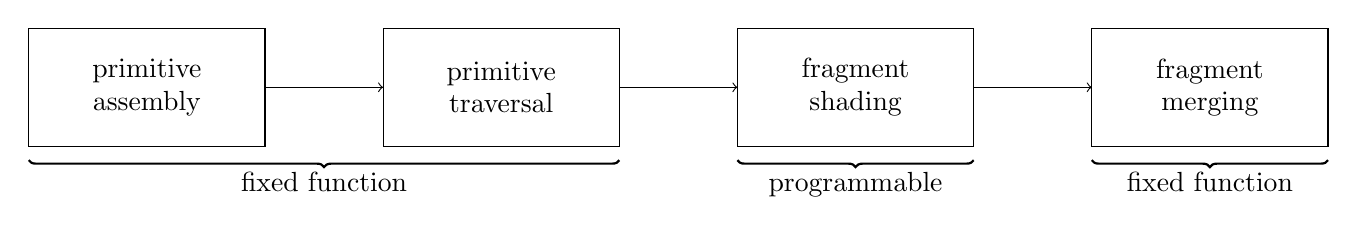
\begin{tikzpicture}[x=0.75cm, y=0.75cm]
                        \draw (0, 0) -- (4, 0) -- (4, -2) -- (0, -2) -- cycle;
                        \draw (6, 0) -- (10, 0) -- (10, -2) -- (6, -2) -- cycle;
                        \draw (12, 0) -- (16, 0) -- (16, -2) -- (12, -2) -- cycle;
                        \draw (18, 0) -- (22, 0) -- (22, -2) -- (18, -2) -- cycle;
                        \node at (2, -1) {\shortstack{primitive\\assembly}};
                        \node at (8, -1) {\shortstack{primitive\\traversal}};
                        \node at (14, -1) {\shortstack{fragment\\shading}};
                        \node at (20, -1) {\shortstack{fragment\\merging}};
                        \draw[
                            thick,
                            decoration={
                                brace,
                                mirror,
                                raise=5
                            },
                            decorate
                        ] (0, -2) -- (10, -2) node[pos=0.5, anchor=north, yshift=-5.55] {fixed function};
                        \draw[
                            thick,
                            decoration={
                                brace,
                                mirror,
                                raise=5
                            },
                            decorate
                        ] (12, -2) -- (16, -2) node[pos=0.5, anchor=north, yshift=-5.55] {programmable};
                        \draw[
                            thick,
                            decoration={
                                brace,
                                mirror,
                                raise=5
                            },
                            decorate
                        ] (18, -2) -- (22, -2) node[pos=0.5, anchor=north, yshift=-5.55] {fixed function};
                        \draw
                        (4, -1) edge[->] (6, -1)
                        (10, -1) edge[->] (12, -1)
                        (16, -1) edge[->] (18, -1);
                    \end{tikzpicture}
                \end{center}
                A lot of merging can be performed at the fragment shading stage.
                Also note that in graphics, we let $(0, 0)$ denote the \textbf{lower left} corner of the window, and we refer to the lower left corner of a pixel.
                For example, the pixel centre (sample location) would be at $(2.5, 1.5)$;
                \begin{center}
                    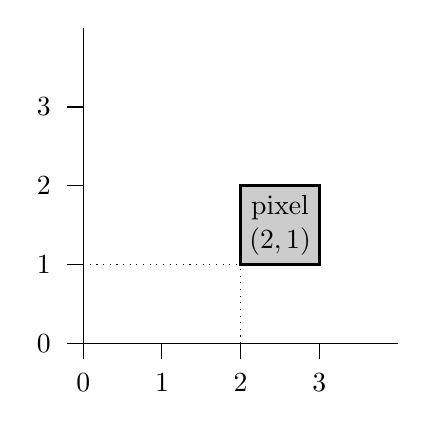
\begin{tikzpicture}
                        \draw
                        (0, 0) -- (0, 4)
                        (0, 0) -- (4, 0);
                        \draw[fill=black!20, very thick] (2, 1) -- (3, 1) -- (3, 2) -- (2, 2) -- cycle;
                        \node at (2.5, 1.5) {\shortstack{pixel\\$(2, 1)$}};
                        \foreach \i in {0,...,3} {
                            \draw (\i, -0.2) -- (\i, 0);
                            \draw (-0.2, \i) -- (0, \i);
                            \node at (\i, -0.5) {\i};
                            \node at (-0.5, \i) {\i};
                        }
                        \draw[dotted]
                        (2, 0) -- (2, 1)
                        (0, 1) -- (2, 1);
                    \end{tikzpicture}
                \end{center}
                In the fragment shading step, given the interpolated vertex attributes (output by the vertex shader), the fragment shader computes colour values for each fragment, by applying textures, performing lighting calculations, etc.
                The fragment merging step follows the following pipeline;
                \begin{center}
                    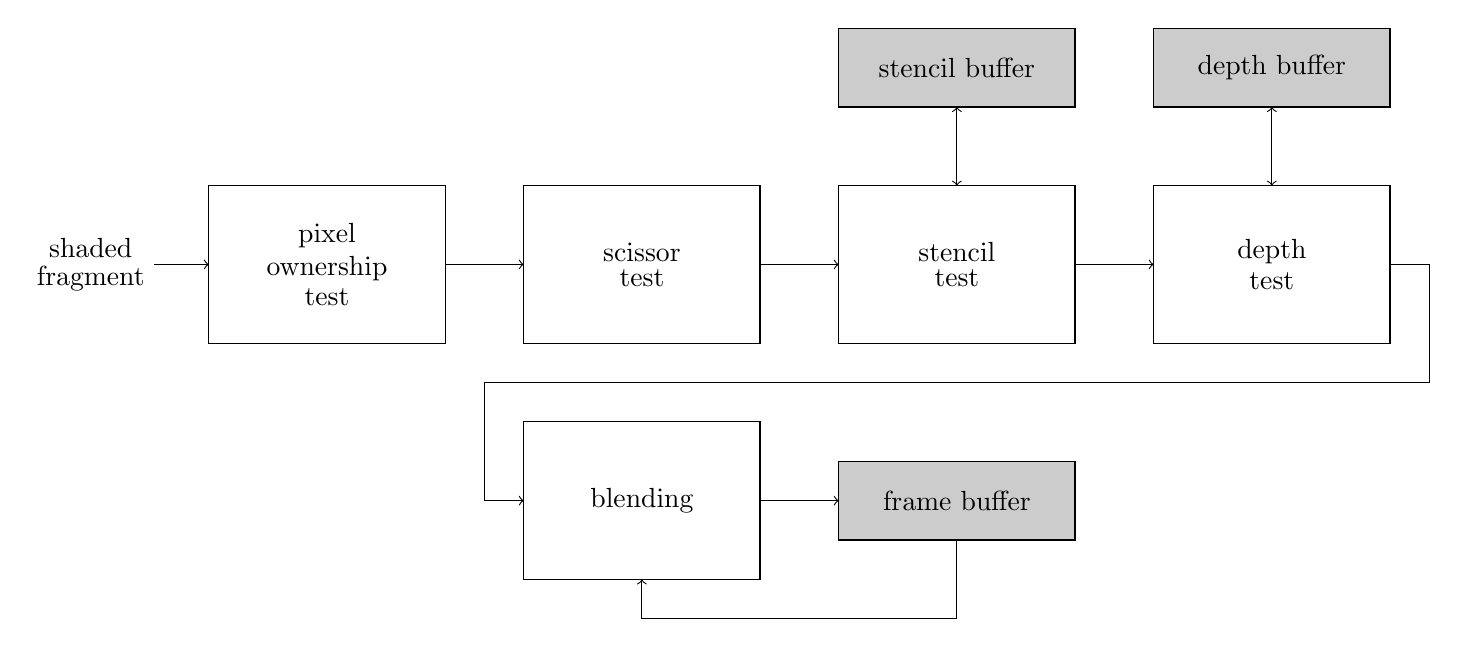
\begin{tikzpicture}
                        \node (sf) at (-1.5, 1) {\shortstack{shaded\\fragment}};
                        \begin{scope}[shift={(0, 0)}]
                            \draw (0, 0) -- (3, 0) -- (3, 2) -- (0, 2) -- cycle;
                            \node at (1.5, 1) {\shortstack{pixel\\ownership\\test}};
                        \end{scope}
                        \begin{scope}[shift={(4, 0)}]
                            \draw (0, 0) -- (3, 0) -- (3, 2) -- (0, 2) -- cycle;
                            \node at (1.5, 1) {\shortstack{scissor\\test}};
                        \end{scope}
                        \begin{scope}[shift={(8, 0)}]
                            \draw (0, 0) -- (3, 0) -- (3, 2) -- (0, 2) -- cycle;
                            \node at (1.5, 1) {\shortstack{stencil\\test}};
                        \end{scope}
                        \begin{scope}[shift={(12, 0)}]
                            \draw (0, 0) -- (3, 0) -- (3, 2) -- (0, 2) -- cycle;
                            \node at (1.5, 1) {\shortstack{depth\\test}};
                        \end{scope}
                        \begin{scope}[shift={(4, -3)}]
                            \draw (0, 0) -- (3, 0) -- (3, 2) -- (0, 2) -- cycle;
                            \node at (1.5, 1) {\shortstack{blending}};
                        \end{scope}
                        \begin{scope}[shift={(8, 3)}]
                            \draw[fill=black!20] (0, 0) -- (3, 0) -- (3, 1) -- (0, 1) -- cycle;
                            \node at (1.5, 0.5) {stencil buffer};
                        \end{scope}
                        \begin{scope}[shift={(12, 3)}]
                            \draw[fill=black!20] (0, 0) -- (3, 0) -- (3, 1) -- (0, 1) -- cycle;
                            \node at (1.5, 0.5) {depth buffer};
                        \end{scope}
                        \begin{scope}[shift={(8, -2.5)}]
                            \draw[fill=black!20] (0, 0) -- (3, 0) -- (3, 1) -- (0, 1) -- cycle;
                            \node at (1.5, 0.5) {frame buffer};
                        \end{scope}
                        \draw
                        (sf) edge[->] (0, 1)
                        (3, 1) edge[->] (4, 1)
                        (7, 1) edge[->] (8, 1)
                        (11, 1) edge[->] (12, 1)
                        (15, 1) -- (15.5, 1) -- (15.5, -0.5) -- (3.5, -0.5) -- (3.5, -2) edge[->] (4, -2)
                        (7, -2) edge[->] (8, -2)
                        (9.5, -2.5) -- (9.5, -3.5) -- (5.5, -3.5) edge[->] (5.5, -3)
                        (9.5, 2) edge[<->] (9.5, 3)
                        (13.5, 2) edge[<->] (13.5, 3);
                    \end{tikzpicture}
                \end{center}
                At this point, we have everything in the frame buffer, generally in the RGBA format, ready for the display stage.
            \subsubsection*{Considerations with Pipeline}
                It's important to keep in mind that the size of the pipeline grows.
                While we may start with a few million vertices in a complex scene, the rasterizer may lead to billions of fragments / pixel candidates.
                Another note is that the vertex and fragment processing stages are highly parallel.
                Instead of iterating over the incoming list of vertices, we write programs that work on an individual vertex, for the GPU to perform in parallel (which is the power of GPU programming) - a similar concept applies for the fragment processing stage.
            \subsubsection*{Architectural Overview}
                It's important to note that graphics hardware is a shared resource.
                The user mode driver (UMD) prepares command buffers for the hardware (and also provides a unified interface for different hardware), which is then submitted to the hardware by the kernel mode driver (KMD).
                The graphics kernel subsystem schedules hardware access.
                \medskip

                The lecture continues with a list of graphics APIs.
        \subsection*{Lecture 5 - Shading Languages}
            \subsubsection*{OpenGL}
                OpenGL is a low-level ``immediate mode'' graphics API specification (and not a library).
                It has a platform independent interface, with a platform dependent implementation.
                It defines an abstract rendering device, which can be operated by a set of functions, and therefore we don't need to care about what the actual hardware is.
                It also uses a \textbf{state machine} for high efficiency.
                In order to write a program, we need to do the following;
                \begin{enumerate}[1.]
                    \itemsep0em
                    \item set up a \textbf{render window} (OS dependent, usually use a library such as \textit{glut}, \textit{Qt}, etc.)
                    \item setup viewport, model transformation, and file I/O (including shaders and textures)
                    \item frame generation (define what happens in every frame)
                \end{enumerate}
                \textbf{Contexts} are abstract graphics devices, which usually do not communicate with each other; each representing one instance of OpenGL.
                There is only one \textbf{current} context per thread.
                We may have multiple OpenGL windows in a single application and they are independent contexts.
                A \textbf{resource} is something that is read from (some sort of data).
                They act as sources of inputs (such as texture images), and sinks for outputs (such as buffers).
                \medskip

                The overall concept uses \textbf{object models}, where objects have unique names (unsigned integer handle).
                Commands work on targets, which has an object \textbf{bound} to the target.
                When a name is bound to a target, the object it identifies becomes current for that target.
                Exceptions exist such as shader objects and program objects, where commands work directly on object names.
                We can consider targets as analogous to types, and commands analogous to methods (drawing analogies to OOP).
            \subsubsection*{Buffer Objects}
                A buffer object stores an array of unformatted memory allocated by the OpenGL context (the GPU) - and they are regular OpenGL objects.
                In order to set up the internal state, it must be bound to the context;
                \begin{lstlisting}
                    void glBindBuffer(enum target, uint bufferName)
                \end{lstlisting}
                To put immutable data on it, the command ~void glBufferStorage(...);~ is used, whereas ~void glBufferData(...);~ is used for mutable data.
                An example is as follows;
                \begin{lstlisting}
                    GLuint my_buffer;

                    // request an unused buffer object name
                    glGenBuffers(1, &my_buffer);

                    // bind name as GL_ARRAY_BUFFER
                    // bound for the first time => creates
                    glBindBuffer(GL_ARRAY_BUFFER, my_buffer);

                    // put some data into my_buffer
                    glBufferStorage(GL_ARRAY_BUFFER, ...);

                    // "unbind" buffer
                    glBindBuffer(GL_ARRAY_BUFFER, 0);

                    // bind it again
                    glBindBuffer(GL_ARRAY_BUFFER, my_buffer);
                    // use it

                    // example of drawing (type, startIdx, number of elements)
                    glDrawArrays(GL_TRIANGLES, 0, 33);

                    // delete buffer object, free resources, release buffer object name
                    glDeleteBuffers(1, &my_buffer);
                \end{lstlisting}
            \subsubsection*{Primitive Types}
                The primitive types available to us are;
                \begin{itemize}
                    \itemsep0em
                    \item ~GL\_POINTS~
                        \begin{center}
                            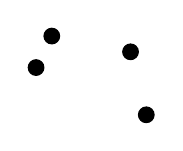
\begin{tikzpicture}
                                \node[rbtb] at (0, 0) {};
                                \node[rbtb] at (1, -0.2) {};
                                \node[rbtb] at (-0.2, -0.4) {};
                                \node[rbtb] at (1.2, -1) {};
                            \end{tikzpicture}
                        \end{center}
                    \item ~GL\_LINES~
                        \begin{center}
                            \begin{tikzpicture}
                                \draw (0, 0) -- (1, 1);
                                \draw (1, 0.7) -- (1.8, -0.1);
                            \end{tikzpicture}
                        \end{center}
                    \item ~GL\_LINE\_STRIP~
                        \begin{center}
                            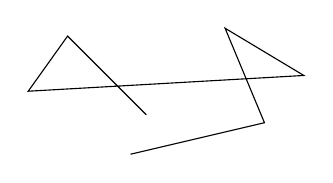
\begin{tikzpicture}
                                \draw (0, 0) -- (-1, 1) -- (-1.5, 0.3) -- (2, 0.5) -- (1, 1.1) -- (1.5, -0.1) -- (-0.2, -0.5);
                            \end{tikzpicture}
                        \end{center}
                    \item ~GL\_LINE\_LOOP~
                        \begin{center}
                            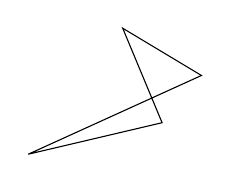
\begin{tikzpicture}
                                \draw (2, 0.5) -- (1, 1.1) -- (1.5, -0.1) -- (-0.2, -0.5) -- cycle;
                            \end{tikzpicture}
                        \end{center}
                    \item ~GL\_POLYGON~
                        \begin{center}
                            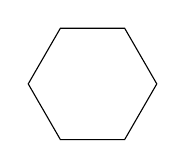
\begin{tikzpicture}
                                \node[
                                    regular polygon,
                                    regular polygon sides=6,
                                    draw,
                                    inner sep=0.5cm,
                                ] (hexagon) {};
                            \end{tikzpicture}
                        \end{center}
                    \item ~GL\_TRIANGLE\_STRIP~
                        \begin{center}
                            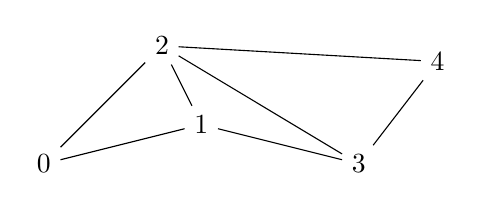
\begin{tikzpicture}
                                \node (a) at (0, 0) {0};
                                \node (b) at (2, 0.5) {1};
                                \node (c) at (1.5, 1.5) {2};
                                \node (d) at (4, 0) {3};
                                \node (e) at (5, 1.3) {4};
                                \draw
                                (a) -- (b) -- (c) -- (a)
                                (b) -- (d) -- (e) -- (c) -- (d);
                            \end{tikzpicture}
                        \end{center}
                        It's important to note that here we alternate between identifying vertices; starting with a counter clockwise ordering, then clockwise, and so on.
                        For example, the first triangle will be 0, 1, 2, then the second triangle is 1, 2, 3, and then the third triangle is 2, 3, 4.
                        This allows vertices to be shared, and is therefore more memory efficient.
                    \item ~GL\_TRIANGLES~
                        \begin{center}
                            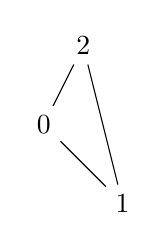
\begin{tikzpicture}
                                \node (a) at (0, 0) {0};
                                \node (b) at (1, -1) {1};
                                \node (c) at (0.5, 1) {2};
                                \draw (a) -- (b) -- (c) -- (a);
                            \end{tikzpicture}
                        \end{center}
                        It's important to note that here we identify vertices counter clockwise (the triangle is 0, 1, 2).
                    \item ~GL\_TRIANGLE\_FAN~
                        \begin{center}
                            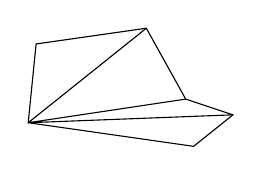
\begin{tikzpicture}
                                \draw (0, 0) -- (0.1, 1) -- (1.5, 1.2) -- (2, 0.3) -- (2.6, 0.1) -- (2.1, -0.3) -- cycle;
                                \draw
                                (0, 0) -- (1.5, 1.2)
                                (0, 0) -- (2, 0.3)
                                (0, 0) -- (2.6, 0.1);
                            \end{tikzpicture}
                        \end{center}
                    \item ~GL\_QUADS~
                        \begin{center}
                            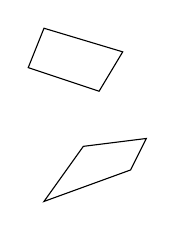
\begin{tikzpicture}
                                \draw (0, 0) -- (1, -0.3) -- (0.7, -0.8) -- (-0.2, -0.5) -- cycle;
                                \draw (0.5, -1.5) -- (1.3, -1.4) -- (1.1, -1.8) -- (0, -2.2) -- cycle;
                            \end{tikzpicture}
                        \end{center}
                    \item ~GL\_QUAD\_STRIP~
                        \begin{center}
                            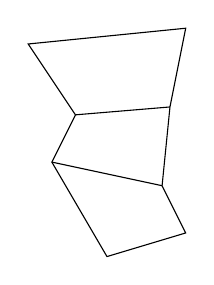
\begin{tikzpicture}
                                \draw (0, 0) -- (2, 0.2) -- (1.8, -0.8) -- (1.7, -1.8) -- (2, -2.4) -- (1, -2.7) -- (0.3, -1.5) -- (0.6, -0.9) -- cycle;
                                \draw
                                (1.8, -0.8) -- (0.6, -0.9)
                                (1.7, -1.8) -- (0.3, -1.5);
                            \end{tikzpicture}
                        \end{center}
                \end{itemize}
                A draw call, which isn't used after OpenGL 4, is done as follows;
                \begin{lstlisting}
                    glBegin(GL_TRIANGLE_STRIP); // primitive type
                    glColor3f(0.0, 1.0, 0.0); // colour state
                    glVertex3f(1.0, 0.0, 0.0); // vertex index
                    ...
                    glEnd();
                \end{lstlisting}
                The more efficient method of doing it is to do the following (using buffer objects) for continuous groups of vertices;
                \begin{lstlisting}
                    glDrawArrays(GL_TRIANGLES, 0, num_vertices);
                \end{lstlisting}
            \subsubsection*{Shaders}
                A shader is a piece of code that can be put in the graphics pipeline.
                To create a vertex or fragment shader, the following has to be done (anything that's not `filled in' will default to fixed functions);
                \begin{center}
                    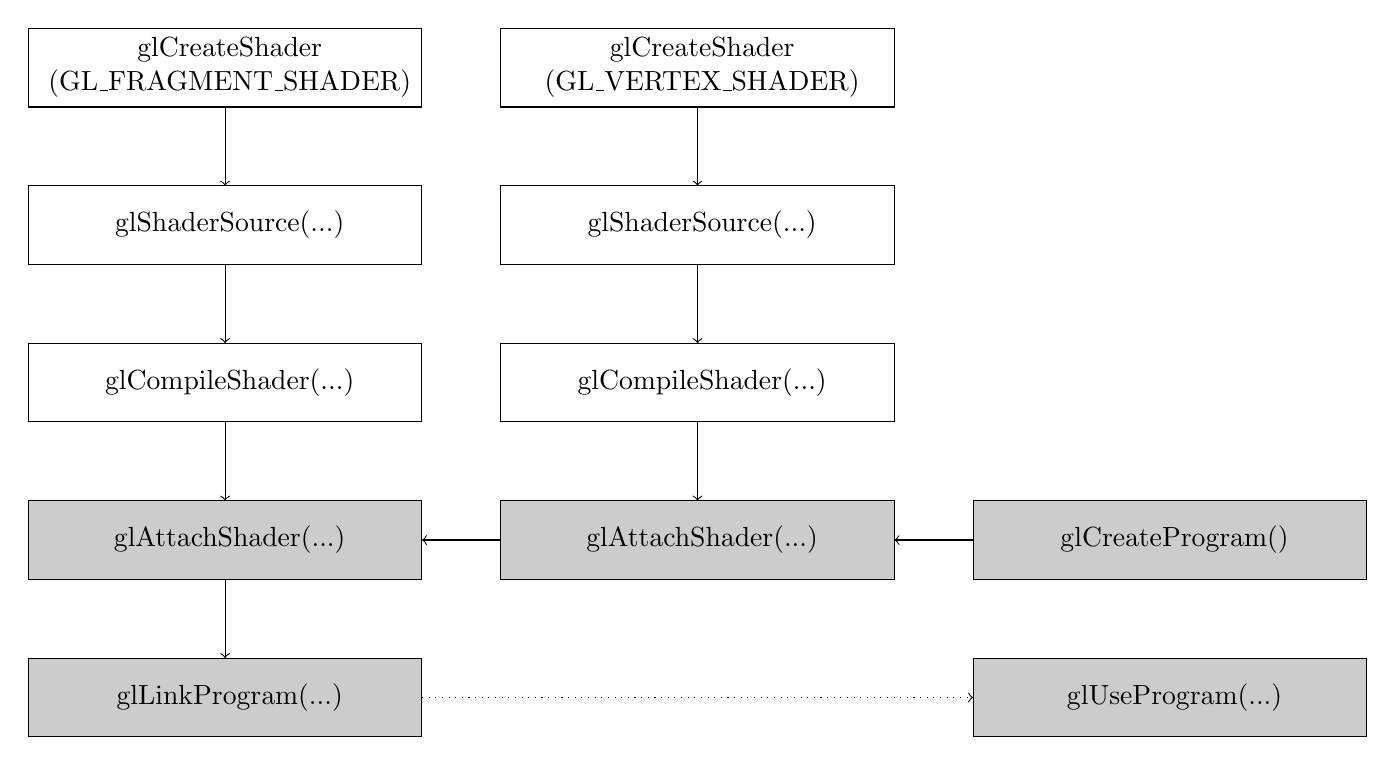
\begin{tikzpicture}
                        \begin{scope}[shift={(0, 0)}]
                            \draw (0, 0) -- (5, 0) -- (5, 1) -- (0, 1) -- cycle;
                            \node at (2.5, 0.5) {\shortstack{~glCreateShader~\\~(GL\_FRAGMENT\_SHADER)~}};
                        \end{scope}
                        \begin{scope}[shift={(0, -2)}]
                            \draw (0, 0) -- (5, 0) -- (5, 1) -- (0, 1) -- cycle;
                            \node at (2.5, 0.5) {~glShaderSource(...)~};
                        \end{scope}
                        \begin{scope}[shift={(0, -4)}]
                            \draw (0, 0) -- (5, 0) -- (5, 1) -- (0, 1) -- cycle;
                            \node at (2.5, 0.5) {~glCompileShader(...)~};
                        \end{scope}
                        \begin{scope}[shift={(0, -6)}]
                            \draw[fill=black!20] (0, 0) -- (5, 0) -- (5, 1) -- (0, 1) -- cycle;
                            \node at (2.5, 0.5) {~glAttachShader(...)~};
                        \end{scope}
                        \begin{scope}[shift={(6, 0)}]
                            \draw (0, 0) -- (5, 0) -- (5, 1) -- (0, 1) -- cycle;
                            \node at (2.5, 0.5) {\shortstack{~glCreateShader~\\~(GL\_VERTEX\_SHADER)~}};
                        \end{scope}
                        \begin{scope}[shift={(6, -2)}]
                            \draw (0, 0) -- (5, 0) -- (5, 1) -- (0, 1) -- cycle;
                            \node at (2.5, 0.5) {~glShaderSource(...)~};
                        \end{scope}
                        \begin{scope}[shift={(6, -4)}]
                            \draw (0, 0) -- (5, 0) -- (5, 1) -- (0, 1) -- cycle;
                            \node at (2.5, 0.5) {~glCompileShader(...)~};
                        \end{scope}
                        \begin{scope}[shift={(6, -6)}]
                            \draw[fill=black!20] (0, 0) -- (5, 0) -- (5, 1) -- (0, 1) -- cycle;
                            \node at (2.5, 0.5) {~glAttachShader(...)~};
                        \end{scope}
                        \begin{scope}[shift={(12, -6)}]
                            \draw[fill=black!20] (0, 0) -- (5, 0) -- (5, 1) -- (0, 1) -- cycle;
                            \node at (2.5, 0.5) {~glCreateProgram()~};
                        \end{scope}
                        \begin{scope}[shift={(0, -8)}]
                            \draw[fill=black!20] (0, 0) -- (5, 0) -- (5, 1) -- (0, 1) -- cycle;
                            \node at (2.5, 0.5) {~glLinkProgram(...)~};
                        \end{scope}
                        \begin{scope}[shift={(12, -8)}]
                            \draw[fill=black!20] (0, 0) -- (5, 0) -- (5, 1) -- (0, 1) -- cycle;
                            \node at (2.5, 0.5) {~glUseProgram(...)~};
                        \end{scope}
                        \draw
                        (12, -5.5) edge[->] (11, -5.5)
                        (6, -5.5) edge[->] (5, -5.5)
                        (5, -7.5) edge[dotted, ->] (12, -7.5)
                        (2.5, 0) edge[->] (2.5, -1)
                        (2.5, -2) edge[->] (2.5, -3)
                        (2.5, -4) edge[->] (2.5, -5)
                        (2.5, -6) edge[->] (2.5, -7)
                        (8.5, 0) edge[->] (8.5, -1)
                        (8.5, -2) edge[->] (8.5, -3)
                        (8.5, -4) edge[->] (8.5, -5);
                    \end{tikzpicture}
                \end{center}
            \subsubsection*{GLSL}
                We have the following types available, initialised with C++ style constructors (~vec3 a = vec3(1.0, 2.0, 3.0);~);
                \begin{itemize}
                    \itemsep0em
                    \item \textbf{scalar types} \hfill ~float~, ~int~, ~bool~
                    \item \textbf{vector types} \hfill ~vec2~, ~vec3~, ~vec4~, ~ivec2~, ~ivec3~, ~ivec4~, ~bvec2~, ~bvec3~, ~bvec4~
                    \item \textbf{matrix types} \hfill ~mat2~, ~mat3~, ~mat4~
                    \item \textbf{texture sampling} \hfill ~sampler1D~, ~sampler2D~, ~sampler3D~, ~samplerCube~
                        \smallskip

                        Specific piece of hardware that does memory access very efficiently.
                \end{itemize}
                The standard C/C++ arithmetic and logic operators hold, as well as operators being overloaded for matrix and vector operations;
                \begin{lstlisting}
                    mat4 m;
                    vec4 a, b, c;

                    b = a*m;
                    c = m*a;
                \end{lstlisting}
                Vectors can be accessed via index (~[]~), ~xyzw~, ~rgba~, or ~stpq~, therefore;
                \begin{lstlisting}
                    vec3 v;
                    v[1] == v.y == v.g == v.t
                \end{lstlisting}
                Swizzling is the following (not really mentioned in detail) - asking for objects in a different order;
                \begin{lstlisting}
                    vec3 a, b;
                    a.xy = b.yx;
                \end{lstlisting}
                ~in~ and ~out ~ copy vertex attributes and other variables to / from shaders (they need to match the next step of the pipeline), whereas ~uniform~ denotes a variable from the application;
                \begin{lstlisting}
                    in vec2 tex_coord;
                    out vec4 colour;

                    uniform float time;
                    uniform vec4 rotation;
                \end{lstlisting}
                We are also given some functions;
                \begin{itemize}
                    \itemsep0em
                    \item \textbf{arithmetic} \hfill e.g. ~sqrt~, ~power~, ~abs~
                    \item \textbf{trigonometric} \hfill e.g. ~sin~, ~asin~
                    \item \textbf{graphical} \hfill e.g. ~length~, ~reflect~
                    \item users can also define functions
                \end{itemize}
                Built-in variables include ~gl\_Position~ which denotes the output position from the vertex shader, and ~gl\_FragColor~, denoting the output colour from the fragment shader.
                This is only for ES, WebGL, and older versions of GLSL (present versions use an out variable).
                \medskip

                The anatomy of a GLSL shader is as follows;
                \begin{lstlisting}
                    #version 400

                    uniform mat4 some_uniform // set by application (configuration values e.g. MVP Matrix)

                    // optional flexible register configuration between shaders (location stuff)
                    layout(location = 0) in vec3 some_input;
                    layout(location = 1) in vec4 another_input;

                    out vec4 some_output; // output definition for next shader stage

                    void main() {

                    }
                \end{lstlisting}
                An example of a fragment shader is as follows;
                \begin{lstlisting}
                    #version 400

                    uniform vec4 ambient;
                    uniform vec4 diffuse;
                    uniform vec4 specular;
                    uniform float shininess;

                    uniform vec4 lightPosition_camSpace; // light position in camera space

                    in fragmentData {
                        vec4 position_camSpace;
                        vec3 normal_camSpace;
                        vec2 textureCoordinate;
                        vec4 color;
                    } frag;

                    out vec4 fragColor;

                    void main(void) {
                        fragColor = frag.color;
                    }
                \end{lstlisting}
        \subsection*{Lecture 6 - Illumination, Shading, and Colour I}
            With very basic illumination, the result is a flat image with a single colour (and we cannot infer a shape).
            We want to give the impression that light acts in a more complex way.
            In local illumination, we focus on how \textbf{one} object interacts with the light sources; we do not consider how objects interact with other objects (such as reflections).
            \subsubsection*{Physics of Shading}
                The light we want to model is whatever is reflected from our object.
                In this lecture, we only consider the brightness at each point.
                Illumination is dependent on various environmental factors, including the properties of the light source;
                \begin{itemize}
                    \itemsep0em
                    \item intensity of emitted light
                    \item distance to the point on the surface (light spreads out)
                \end{itemize}
                As well as object (surface) properties;
                \begin{itemize}
                    \itemsep0em
                    \item surface normal vector
                    \item object position relative to light source
                    \item reflectivity / albedo (ability to absorb light energy) of the surface
                \end{itemize}
            \subsubsection*{Radiometry}
                \begin{align*}
                    e_\lambda & = \frac{hc}{\lambda} & \text{energy of a photon} \\
                    h & \approx 6.63 \times 10^{-34} Js & \text{Planck constant} \\
                    c & \approx 3 \times 10^8 ms^{-1} & \text{speed of light} \\
                    Q & = \summation{i = 1}{n} \frac{hc}{\lambda_i} & \text{radiant energy of $n$ photons} \\
                    \Phi & = \dif{Q}{t} & \text{radiation / electromagnetic / radiant flux (in Watts)}
                \end{align*}
                Radiant flux is the number of photons we have available to reflect at any one time.
                \textbf{Radiance} is defined as the radiant flux per unit solid angle per unit projected area; the number of photons per time at a small area in a particular direction (units are watts per meter$^2$ steradian);
                \begin{center}
                    \begin{tikzpicture}[x=1.25cm, y=1.25cm]
                        \draw
                        (0, 0) edge[->] (0, 2)
                        (0, 0) edge[->] (2, 0)
                        (0, 0) edge[->] (-1.4, -1.4);
                        \draw (-0.3, 0.2) -- (0.7, 0.2) -- (0.2, -0.3) -- (-0.8, -0.3) -- cycle;
                        \begin{scope}[rotate={50}]
                            \draw (0, 0) edge[->] (2.5, 0);
                            \draw (0, 0) -- (2.2, 0.1);
                            \draw (0, 0) -- (2.2, -0.1);
                            \draw (2.2, 0) ellipse (0.04 and 0.1);
                        \end{scope}
                        \node at (0.3, 2) {$z$};
                        \node at (2, -0.3) {$y$};
                        \node at (-1.1, -1.4) {$x$};
                        \node at (0.5, -0.3) {$\mathrm{d}A$};
                        \node at (1.9, 1.9) {$L$};
                        \node at (1.55, 1.4) {$\mathrm{d}\omega$};
                        \draw[<->] (0, 0) ++(50:1) arc (50:90:1);
                        \node at (0.45, 1.2) {$\theta$};
                        \node at (6, 0) {$L(\omega) = \dfrac{\mathrm{d}^2 \Phi}{\cos \theta \mathrm{d} A \mathrm{d} \omega}$};
                    \end{tikzpicture}
                \end{center}
                \textbf{Irradiance} is how much light arrives from any other surface on another surface.
                It is the differential flux falling onto differential area (in Watts per meter$^2$).
                $$E = \dif{\Phi}{A}$$
                It can be seen as a density of incident flux falling onto a surface, and can be obtained by integrating the radiance over the solid angle.
            \subsubsection*{Reflection and Reflectance}
                The actual property we want to model is reflection.
                We want to work out how much is reflected to the viewer.
                \textbf{Reflection} is the process by which electromagnetic flux incident on a surface leaves the surface without a change in frequency (fluorescence), and \textbf{reflectance} is a fraction of the incident flux that is reflected.
                We do not consider absorption, transmission nor diffraction.
                \medskip

                We want to find out how much is reflected when $E_i$ reaches an infinitely small patch of surface.
                To model this, we need the Bidirectional Reflectance Distribution Function (BRDF) (also seen in \textbf{CO316}) - the units are steradian$^{-1}$;
                $$f_r(\theta_i, \phi_i, \theta_r, \phi_r) = \dif{L_r(\theta_r, \phi_r)}{E_i(\theta_i, \phi_i)}$$
                In this case, $L_r$ is the viewer, and $E_i$ the light source.
                \medskip

                Given our surface is well behaved and generally flat, we can simplify it by stating that a rotation along the surface normal does not change the reflectance;
                $$f_r(\theta_i, \theta_r, \phi_r - \phi_i) = f_r(\theta_i, \theta_r, \phi_d) = \dif{L_r(\theta_r, \phi_d)}{(\theta_i, \phi_d)}$$
                However, this isn't true for surfaces with strongly oriented nanostructures (such as \textit{vantablack}, hair, fur, velvet).
                The properties of BRDFs are as follows;
                \begin{itemize}
                    \itemsep0em
                    \item non-negative
                        $$f_r(\theta_i, \phi_i, \theta_r, \phi_r) \geq 0$$
                    \item energy conservation \hfill we never have more light come out than comes in
                        $$\forall \theta_i, \phi_i\ \defint{\Omega}{}{f_r(\theta_i, \phi_i, \theta_r, \phi_r)}{\mu(\theta_r, \phi_r)} \leq 1$$
                    \item reciprocity
                        $$f_r(\theta_i, \phi_i, \theta_r, \phi_r) = f_r(\theta_r, \phi_r, \theta_i, \phi_i)$$
                \end{itemize}
                In our case, we only consider the discrete version to compute reflected radiance (with $n$ point light sources)- note that $\Phi_{s, j}$ denotes radiant flux, and $d_j$ is the distance;
                $$L_r(\omega_r) = \summation{j = 1}{n} f_r(\omega_{i, j}, \omega_r) E_j = \summation{j = 1}{n} f_r(\omega_{i, j}, \omega_r) \cos \theta_j \frac{\Phi_{s, j}}{4 \pi d_j^2} $$
                Some cases;
                \begin{itemize}
                    \itemsep0em
                    \item \textbf{ideal diffuse reflectance} \hfill depends on light source position and surface normal
                        \smallskip

                        In this case we define BRDF as a constant.
                        The only dependence is the position of our light, and how that is related to the normal vector of our surface.
                        At a microscopic level, an ideal diffuse surface is very rough (such as chalk, clay, or some paints).
                        \begin{center}
                            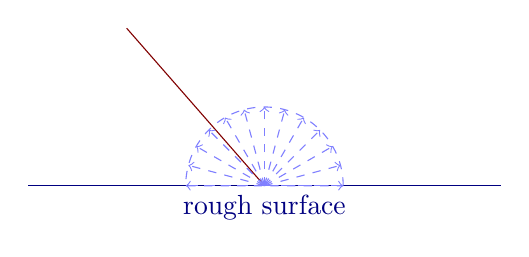
\begin{tikzpicture}
                                \draw[blue!50!black] (0, 0) edge[below] node{rough surface} (6, 0);
                                \draw[red!50!black] (1.25, 2) edge[->] (3, 0);
                                \draw[dashed, blue!50]
                                (4, 0) arc(0:180:1) -- cycle
                                (3, 0) edge[->] +(0:1)
                                (3, 0) edge[->] +(15:1)
                                (3, 0) edge[->] +(30:1)
                                (3, 0) edge[->] +(45:1)
                                (3, 0) edge[->] +(60:1)
                                (3, 0) edge[->] +(75:1)
                                (3, 0) edge[->] +(90:1)
                                (3, 0) edge[->] +(105:1)
                                (3, 0) edge[->] +(120:1)
                                (3, 0) edge[->] +(135:1)
                                (3, 0) edge[->] +(150:1)
                                (3, 0) edge[->] +(165:1)
                                (3, 0) edge[->] +(180:1);
                            \end{tikzpicture}
                        \end{center}
                        This has a constant BRDF value;
                        \begin{align*}
                            L_r(\omega_r) & = \defint{\Omega}{}{f_r{\omega_i, \omega_r}}{E_i{\omega_i}} \\
                            & = f_r \defint{\Omega}{}{}{E_i{\omega_i}} \\
                            & = f_r E_i \\
                            \mathrm{d}B & = \mathrm{d}A \cos \theta_i
                        \end{align*}
                        Using the following, we can see that the reflection is maximal when it is parallel to the normal, and minimal when it is perpendicular;
                        \begin{center}
                            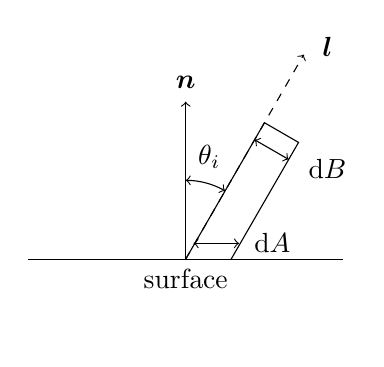
\begin{tikzpicture}
                                \begin{scope}[shift={(2, 0)}, rotate={-30}]
                                    \draw (0, 1.75) edge[<->] (0.5, 1.75);
                                    \draw (0, 0) -- (0.5, 0) -- (0.5, 2) -- (0, 2) -- cycle;
                                    \draw (0, 0) edge[dashed, ->] (0, 3);
                                \end{scope}
                                \node at (3.8, 2.7) {$\vec{l}$};
                                \draw[white, fill=white] (0, 0) -- (4, 0) -- (4, -1) -- (0, -1) -- cycle;
                                \draw (0, 0) edge[below] node{surface} (4, 0);
                                \draw (2, 0) edge[->] (2, 2);
                                \node at (2, 2.25) {$\vec{n}$};
                                \draw[<->] (2, 0) ++(60:1) arc (60:90:1);
                                \node at (2.3, 1.3) {$\theta_i$};
                                \begin{scope}[shift={(0.1, 0.2)}]
                                    \draw (2, 0) edge[<->] (2.577, 0);
                                \end{scope}
                                \node at (3.1, 0.2) {$\mathrm{d}A$};
                                \node at (3.8, 1.15) {$\mathrm{d}B$};
                            \end{tikzpicture}
                        \end{center}
                        These reflectors reflect light according to \textbf{Lambert's cosine law}; the more parallel the light is to the normal, the higher the strength of the outgoing light.
                        This is physically incorrect, but it is an approximation, and gives a basic shading.
                        From a single point light source \textbf{to} direction $\vec{l}$, on a a surface with diffuse reflection coefficient $k_d$ (the colour of the surface in the simplest case) and surface normal $\vec{n}$;
                        $$L(\omega_r) = k_d (\vec{n} \cdot \vec{l}) \frac{\Phi_s}{4 \pi d^2}$$
                        The direction \textbf{vectors must be normalised}.
                        Note that from this point on, using $\vec{n} \cdot \vec{l}$ denotes $\max(\vec{n} \cdot \vec{l}, 0)$; ensuring that the result is at least 0.
                    \item \textbf{ideal specular reflectance} \hfill depends on light source position, surface normal, and viewpoint position
                        \smallskip

                        In contrast to diffuse, reflection is \textbf{only} at mirror angle, and is view dependent.
                        Nanostructures of the surface are usually oriented in the same direction as the surface (such as polished metals or mirrors).
                        \begin{center}
                            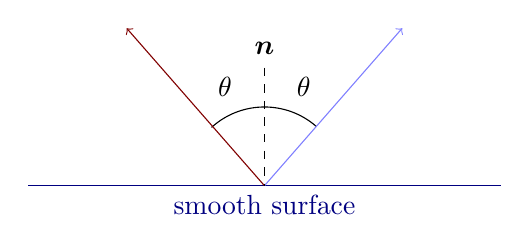
\begin{tikzpicture}
                                \draw (3, 0) ++(48.8:1) arc (48.8:132.2:1);
                                \draw[blue!50!black] (0, 0) edge[below] node{smooth surface} (6, 0);
                                \draw[red!50!black] (1.25, 2) edge[<-] (3, 0);
                                \draw[blue!50] (4.75, 2) edge[<-] (3, 0);
                                \draw[dashed] (3, 1.5) -- (3, 0);

                                \node at (3, 1.75) {$\vec{n}$};
                                \node at (2.5, 1.25) {$\theta$};
                                \node at (3.5, 1.25) {$\theta$};
                            \end{tikzpicture}
                        \end{center}
                        This uses a special case of Snell's law, where the incoming ray, the surface normal, and reflected ray are all on a common plane;
                        \begin{align*}
                            n_l \sin \theta_l & = n_r \sin \theta_r \\
                            n_l & = n_r  \\
                            \theta_l & = \theta_r
                        \end{align*}
                        What we want to do is figure out how our viewpoint is related to the reflectance direction.
                    \item \textbf{non-ideal reflectors}
                        \smallskip

                        In the real world, materials are neither ideal mirror reflectors following Snell's law, nor ideal diffuse surfaces.
                        A simple empirical model expects most of the light reflected to travel in the direction of the ideal ray; however due to surface nanostructures some of the light can be expected to be reflected slightly offset from the ideal.
                        As we move further out (in the angular sense) from the reflected ray, we expect to see less light reflected.
                        \begin{center}
                            \hfill
                            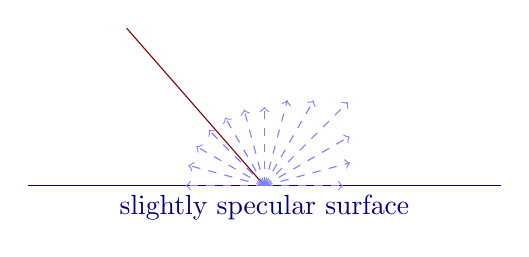
\begin{tikzpicture}
                                \draw[blue!50!black] (0, 0) edge[below] node{slightly specular surface} (6, 0);
                                \draw[red!50!black] (1.25, 2) edge[->] (3, 0);
                                \draw[dashed, blue!50]
                                (3, 0) edge[->] +(0:1)
                                (3, 0) edge[->] +(15:1.125)
                                (3, 0) edge[->] +(30:1.25)
                                (3, 0) edge[->] +(45:1.5)
                                (3, 0) edge[->] +(60:1.25)
                                (3, 0) edge[->] +(75:1.125)
                                (3, 0) edge[->] +(90:1)
                                (3, 0) edge[->] +(105:1)
                                (3, 0) edge[->] +(120:1)
                                (3, 0) edge[->] +(135:1)
                                (3, 0) edge[->] +(150:1)
                                (3, 0) edge[->] +(165:1)
                                (3, 0) edge[->] +(180:1);
                            \end{tikzpicture}
                            \hfill
                            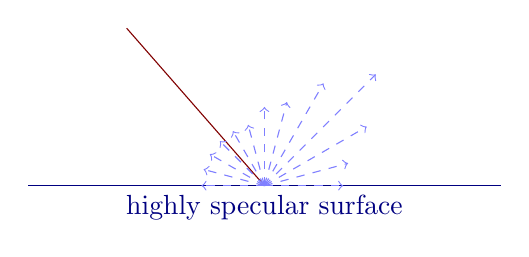
\begin{tikzpicture}
                                \draw[blue!50!black] (0, 0) edge[below] node{highly specular surface} (6, 0);
                                \draw[red!50!black] (1.25, 2) edge[->] (3, 0);
                                \draw[dashed, blue!50]
                                (3, 0) edge[->] +(0:1)
                                (3, 0) edge[->] +(15:1.1)
                                (3, 0) edge[->] +(30:1.5)
                                (3, 0) edge[->] +(45:2)
                                (3, 0) edge[->] +(60:1.5)
                                (3, 0) edge[->] +(75:1.1)
                                (3, 0) edge[->] +(90:1)
                                (3, 0) edge[->] +(105:0.8)
                                (3, 0) edge[->] +(120:0.8)
                                (3, 0) edge[->] +(135:0.8)
                                (3, 0) edge[->] +(150:0.8)
                                (3, 0) edge[->] +(165:0.8)
                                (3, 0) edge[->] +(180:0.8);
                            \end{tikzpicture}
                            \hfill \phantom{}
                        \end{center}
                        In the case of the slightly shiny surface, there is slightly higher intensity in the reflected direction, however in the highly shiny surface, there is high intensity in the reflected direction.
                        \medskip

                        The \textbf{Phong} model states that the closer the viewer direction $\alpha$ is to the ideal reflection direction, the brighter the light should appear.
                        \begin{center}
                            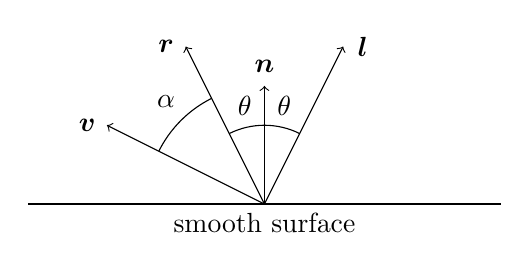
\begin{tikzpicture}
                                \draw (3, 0) ++(63.4:1) arc (63.4:116.6:1);
                                \draw (0, 0) edge[below] node{smooth surface} (6, 0);
                                \draw (2, 2) edge[<-] (3, 0);
                                \draw (4, 2) edge[<-] (3, 0);
                                \draw (1, 1) edge[<-] (3, 0);
                                \draw (3, 0) ++(116.6:1.5) arc (116.6:153.4:1.5);
                                \draw (3, 1.5) edge[<-] (3, 0);

                                \node at (0.75, 1) {$\vec{v}$};
                                \node at (3, 1.75) {$\vec{n}$};
                                \node at (1.75, 2) {$\vec{r}$};
                                \node at (4.25, 2) {$\vec{l}$};
                                \node at (2.75, 1.25) {$\theta$};
                                \node at (3.25, 1.25) {$\theta$};
                                \node at (1.75, 1.3) {$\alpha$};
                            \end{tikzpicture}
                        \end{center}
                        Therefore we have the following, where $k_s$ is the specular reflection coefficient, and $q$ the specular reflection exponent;
                        $$L(\omega_r) = k_s (\cos \alpha)^q \frac{\Phi_s}{4 \pi d^2} = k_s (\vec{v} \cdot \vec{r})^q \frac{\Phi_s}{4 \pi d^2}$$
                        A higher $q$ leads to a more focused light (a shiner surface), and $k_s$ is the surface property we want to manipulate.
                        In order to obtain $\vec{r}$, we can calculate the following;
                        \begin{align*}
                            \vec{r} + \vec{l} & = 2 \cos \theta \vec{n} & \Rightarrow \\
                            \vec{r} & = 2(\vec{n} \cdot \vec{l}) \vec{n} - \vec{l} \\
                            L(\omega_r) & = k_s (\vec{v} \cdot (2(\vec{n} \cdot \vec{l}) \vec{n} - \vec{l}))^q \frac{\Phi_s}{4 \pi d^2}
                        \end{align*}
                        The \textbf{Blinn-Phong} variation uses the halfway vector $\vec{h}$ between $\vec{l}$ and $\vec{v}$;
                        \begin{align*}
                            \vec{h} & = \frac{\vec{l} + \vec{v}}{|| \vec{l} + \vec{v} ||} \\
                            L(\omega_r) & = k_s (\cos \beta)^q \frac{\Phi_s}{4 \pi d^2} \\
                            & = k_s (\vec{n} \cdot \vec{h})^q \frac{\Phi_s}{4 \pi d^2}
                        \end{align*}
                    \item \textbf{ambient}
                        \smallskip

                        This represents the reflection of all indirect illumination (it is a hack).
                        This avoids the complexity of global illumination;
                        $$L(\omega_r) = k_a$$
                \end{itemize}
                The Phong model is a sum of three components; the \teal{ambient}, the \violet{diffuse} reflection, and the \blue{specular} reflection.
                $$L(\omega_r) = \teal{k_a} + (\violet{k_d (\vec{n} \cdot \vec{l})} + \blue{k_s (\vec{v} \cdot \vec{r})^q}) \frac{\Phi_s}{4 \pi d^2}$$
            \subsubsection*{Note on Inverse Square Law}
                Light falls off according to an inverse square law, hence the $d^2$ term.
                However, it may not produce the best results, and we can instead often use $(d + s)$ in place, where $s$ is a heuristic constant.
            \subsubsection*{Shading}
                The three levels at which shading can be applied in polygon based systems, providing increasing realism at the cost of computation, are;
                \begin{itemize}
                    \itemsep0em
                    \item \textbf{flat shading}
                        \smallskip

                        This can be done wherever.
                        Each polygon is shaded uniformly over is surface, and computed by taking a point in the centre and at the surface normal (consider a light source at infinity).
                        Normally, only the diffuse and ambient components are used
                    \item \textbf{Gouraud shading}
                        \smallskip

                        Interpolates colour across triangles.
                        This is fast, and supported by most GPUs, but cannot accurately model specular components (since we don't have normal vectors at each point on a polygon).
                    \item \textbf{Phong shading} \hfill fragment stage
                        \smallskip

                        Interpolates normals across triangles; more accurate modelling of specular components, but slower.
                \end{itemize}
                \textbf{Interpolation shading} is a more accurate way to render a shaded polygon, by computing an independent shade at each point;
                \begin{enumerate}[1.]
                    \itemsep0em
                    \item compute a shade value at each vertex
                    \item interpolate to find shade value at the boundary \hfill $L = \frac{d_1 L_3 + d_2 L_1}{d_1 + d_2}$
                        \begin{center}
                            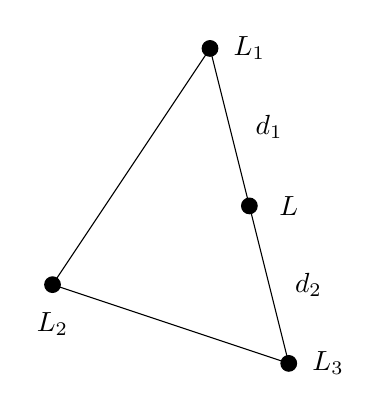
\begin{tikzpicture}
                                \draw (0, 0) -- (2, 3) -- (3, -1) -- cycle;
                                \node[rbtb] at (0, 0) {};
                                \node[rbtb] at (2, 3) {};
                                \node[rbtb] at (3, -1) {};
                                \node[rbtb] at (2.5, 1) {};
                                \node at (2.5, 3) {$L_1$};
                                \node at (0, -0.5) {$L_2$};
                                \node at (3.5, -1) {$L_3$};
                                \node at (3, 1) {$L$};
                                \node at (2.75, 2) {$d_1$};
                                \node at (3.25, 0) {$d_2$};
                            \end{tikzpicture}
                        \end{center}
                    \item interpolate to find shade values in the middle \hfill $L = \frac{d_1 L_B + d_2 L_A}{d_1 + d_2}$
                        \begin{center}
                            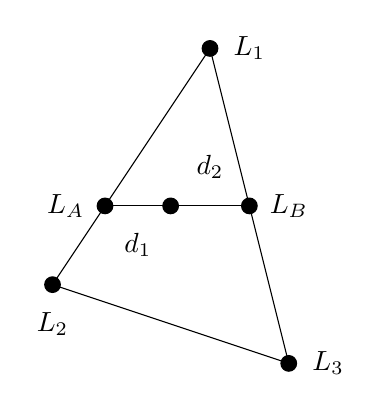
\begin{tikzpicture}
                                \draw (0, 0) -- (2, 3) -- (3, -1) -- cycle;
                                \node[rbtb] at (0, 0) {};
                                \node[rbtb] at (2, 3) {};
                                \node[rbtb] at (3, -1) {};
                                \node[rbtb] at (2.5, 1) {};
                                \node[rbtb] at (2/3, 1) {};
                                \node at (2.5, 3) {$L_1$};
                                \node at (0, -0.5) {$L_2$};
                                \node at (3.5, -1) {$L_3$};
                                \node at (3, 1) {$L_B$};
                                \node at (2/3 - 0.5, 1) {$L_A$};
                                \node[rbtb] at (1.5, 1) {};
                                \draw (2/3, 1) -- (2.5, 1);
                                \node at (1.08333, 0.5) {$d_1$};
                                \node at (2, 1.5) {$d_2$};
                            \end{tikzpicture}
                        \end{center}
                \end{enumerate}
        \subsection*{Lecture 7 - Illumination, Shading, and Colour II}
            Colours are energy distributions.
            Lasers are light sources that contain a single / narrow band of wavelengths.
            Light is made up of a mixture of many wavelengths, with an energy distribution.
            This lecture starts with a lot about colour, similar to \textbf{CO316}.
            The \textbf{tri-stimulus colour theory} states receptor performance implies that colours do not have a unique energy distribution, and more importantly colours which are a distributed over all wavelengths can be matched by mixing red, green, and blue.
            \subsubsection*{Colour Matching}
                Given any colour light source, we can try to match it with a mixture of three light sources (with $R, G, B$ being pure light sources, and $r, g, b$ being their respective intensities);
                $$X = rR + gG + bB$$
                However, not all colours can be matched with a given set of light sources - we cannot model anything that will take out colour.
                \textbf{Subtractive matching} allows us to add light to the colour we are trying to match, for example;
                $$X + r = g + b$$
                Printed documents cannot emit light, and are examples of subtractive matching (as opposed to mixing light emitters such as screens, which is additive matching).
            \subsubsection*{CIE Diagram}
                The CIE diagram was devised as a standard normalised representation of colours.
                Consider normalising the ranges between 0 and 1.
                The colours can be normalised such that the components sum to 1;
                \begin{align*}
                    x & = \frac{r}{r + g + b} \\
                    y & = \frac{g}{r + g + b} \\
                    z & = \frac{b}{r + g + b} \\
                    & = 1 - x - y
                \end{align*}
                This has the following representation, where we have the hypothetical sources as follows;
                \begin{center}
                    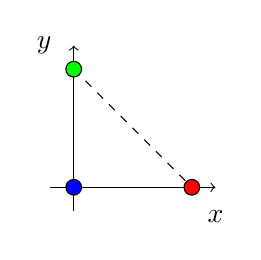
\begin{tikzpicture}[x=1.5cm, y=1.5cm]
                        \draw
                        (0, -0.2) edge[->] (0, 1.2)
                        (-0.2, 0) edge[->] (1.2, 0)
                        (0, 1) edge[dashed] (1, 0);
                        \node[inner sep=2pt, circle, draw=black, fill=red] at (1, 0) {};
                        \node[inner sep=2pt, circle, draw=black, fill=green] at (0, 1) {};
                        \node[inner sep=2pt, circle, draw=black, fill=blue] at (0, 0) {};
                        \node at (-0.25, 1.2) {$y$};
                        \node at (1.2, -0.25) {$x$};
                    \end{tikzpicture}
                \end{center}
                However, the actual visible colours are a subset of this, done through manual testing.
                The pure colours (coherent $\lambda$) are around the edge of the diagram.
                In addition, the shape must be convex, since any blend would produce a colour in the visible region.
                When the three colours are components are equal, the colour is white ($x = y \approx 0.33$).
                Pure colours are fully saturated (colours on the edge of the horseshoe), and a line from the pure colour $P$ going through the white point $W$ will cross over on the other side at a \textbf{complement colour} $C$.
            \subsubsection*{Conversion}
                Converting from RGB (monitor's representation) to CIE is done with the following;
                $$\begin{bmatrix}
                    x \\ y \\ z
                \end{bmatrix} = \begin{bmatrix}
                    0.628 & 0.268 & 0.150 \\
                    0.346 & 0.588 & 0.070 \\
                    0.026 & 0.144 & 0.780
                \end{bmatrix} \begin{bmatrix}
                    R \\ G \\ B
                \end{bmatrix}$$
                A conversion between RGB and HSV is done as follows;
                \begin{align*}
                    V & = \max(r, g, b) \\
                    S & = \frac{\max(r, g, b) - \min(r, g, b)}{\max(r, g, b)} \\
                    H & = \begin{cases}
                        \text{undefined} & r = g = b \\
                        120 \cdot \frac{g - b}{(r - b) + (g - b)} & (r > b) \land (g > b) \\
                        120 + 120 \cdot \frac{b - r}{(g - r) + (b - r)} & (g > r) \land (b > r) \\
                        240 + 120 \cdot \frac{r - g}{(r - g) + (b - g)} & (r > g) \land (b > g)
                    \end{cases}
                \end{align*}
            \subsubsection*{Transparency}
                In addition, we can model transparency with an $\alpha$ channel;
                \begin{itemize}
                    \itemsep0em
                    \item transparent \hfill $\alpha = 0$
                    \item semi-transparent \hfill $0 < \alpha < 1$
                    \item opaque \hfill $\alpha = 1$
                \end{itemize}
        \subsection*{Lecture 8 - Texture Mapping}
            With the current techniques we have, to create any detailed scenery, we'd need to create individual models for small details.
            The solution is to use images, in the form of textures on top of basic models.
            The key is to generate colours from some underlying function;
            \begin{itemize}
                \itemsep0em
                \item one-dimensional functions
                \item two-dimensional functions
                \item three-dimensional functions
                \item raster images (texels) \hfill most common
            \end{itemize}
            A procedural texture maps a function $F(\vec{p})$ to a colour.
            This can be non-intuitive and quite difficult to match real textures.
            \subsubsection*{Photo Textures}
                The idea is to define a 2D coordinate system on an image, which is then mapped onto a 3D object.
                For each fragment on an object's surface, we want to work out what coordinate needs to be sampled in the image's 2D space to get the right colour.
                \medskip

                Conventionally, the texture coordinates are denoted with $(s, t)$, for horizontal and vertical - really just a two-dimensional coordinate system.
                The object surface is similarly denoted with $(u, v)$ and the pixel on the screen denoted with $(x, y)$ - we need to know how the pixel on the screen maps to a $(u, v)$ surface coordinate, and how the surface coordinate maps to a $(s, t)$ texture coordinate.
                Typically, the mapping from $(s, t)$ to $(u, v)$ is manually predefined.
            \subsubsection*{Paramterisation}
                A simple method is planar mapping, where we simply ignore one of the coordinates; however, this only looks good from the front of the object (any other sides will have some sort of smearing artifact).
                Another possible way is to build a cylinder (which can be easily parameterised, similar to a plane), and place the object inside.
                As expected, this works well for mostly cylindrical objects.
                A similar approach is to create a spherical mapping.
                One common method for environment mapping is \textbf{box mapping}.
                This creates a box around the object, which performs six planar mappings (one for each face).
                \medskip

                \textbf{Unwrapping} is the process of creating this manual mapping.
                Typically, all mappings have distortions and singularities, which will often require manual fixing.
            \subsubsection*{Texture Coordinates}
                At each vertex, we specify a texture coordinate.
                The canonical texture coordinates go from $(0, 0)$ to $(1, 1)$.
                When we leave the boundaries of $[0, 1]$, we can take multiple approaches (note that for these examples, for my sake, I'm only drawing a simple $1 \times 3$ image).
                The original texture is the following;
                \begin{center}
                    
\begin{tikzpicture}
                        \draw[fill=black!50] (1, 0) -- (2, 0) -- (2, -1) -- (1, -1) -- cycle;
                        \draw[fill=black] (2, 0) -- (3, 0) -- (3, -1) -- (2, -1) -- cycle;
                        \draw[very thick] (0, 0) -- (3, 0) -- (3, -1) -- (0, -1) -- cycle;
                        \draw[very thick]
                        (1, 0) -- (1, -1)
                        (2, 0) -- (2, -1);
                    \end{tikzpicture}
                \end{center}
                Some of the approaches we can take are as follows, known as \textbf{texture addressing modes};
                \begin{itemize}
                    \itemsep0em
                    \item \textbf{static colour}
                        \begin{center}
                            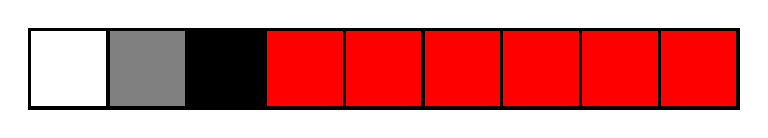
\begin{tikzpicture}
                                \draw[fill=black!50] (1, 0) -- (2, 0) -- (2, -1) -- (1, -1) -- cycle;
                                \draw[fill=black] (2, 0) -- (3, 0) -- (3, -1) -- (2, -1) -- cycle;
                                \draw[fill=red] (3, 0) -- (9, 0) -- (9, -1) -- (3, -1) -- cycle;
                                \draw[very thick] (0, 0) -- (9, 0) -- (9, -1) -- (0, -1) -- cycle;
                                \foreach \x in {1,...,8} {
                                    \draw[very thick] (\x, 0) -- (\x, -1);
                                }
                            \end{tikzpicture}
                        \end{center}
                        Outside the border, we use a static colour (red in this case).
                    \item \textbf{clamped}
                        \begin{center}
                            
\begin{tikzpicture}
                                \draw[fill=black!50] (1, 0) -- (2, 0) -- (2, -1) -- (1, -1) -- cycle;
                                \draw[fill=black] (2, 0) -- (3, 0) -- (3, -1) -- (2, -1) -- cycle;
                                \draw[fill=black] (3, 0) -- (9, 0) -- (9, -1) -- (3, -1) -- cycle;
                                \draw[very thick] (0, 0) -- (9, 0) -- (9, -1) -- (0, -1) -- cycle;
                                \foreach \x in {1,...,8} {
                                    \draw[very thick] (\x, 0) -- (\x, -1);
                                }
                            \end{tikzpicture}
                        \end{center}
                        Outside the border, we use the last colour in the range (black, in this case).
                    \item \textbf{repeated}
                        \begin{center}
                            
\begin{tikzpicture}
                                \begin{scope}
                                    \draw[fill=black!50] (1, 0) -- (2, 0) -- (2, -1) -- (1, -1) -- cycle;
                                    \draw[fill=black] (2, 0) -- (3, 0) -- (3, -1) -- (2, -1) -- cycle;
                                \end{scope}
                                \begin{scope}[shift={(3, 0)}]
                                    \draw[fill=black!50] (1, 0) -- (2, 0) -- (2, -1) -- (1, -1) -- cycle;
                                    \draw[fill=black] (2, 0) -- (3, 0) -- (3, -1) -- (2, -1) -- cycle;
                                \end{scope}
                                \begin{scope}[shift={(6, 0)}]
                                    \draw[fill=black!50] (1, 0) -- (2, 0) -- (2, -1) -- (1, -1) -- cycle;
                                    \draw[fill=black] (2, 0) -- (3, 0) -- (3, -1) -- (2, -1) -- cycle;
                                \end{scope}
                                \draw[very thick] (0, 0) -- (9, 0) -- (9, -1) -- (0, -1) -- cycle;
                                \foreach \x in {1,...,8} {
                                    \draw[very thick] (\x, 0) -- (\x, -1);
                                }
                            \end{tikzpicture}
                        \end{center}
                        Once we exit the range, we simply wrap back to the first coordinate, repeating the texture.
                    \item \textbf{mirrored}
                        \begin{center}
                            
\begin{tikzpicture}
                                \begin{scope}
                                    \draw[fill=black!50] (1, 0) -- (2, 0) -- (2, -1) -- (1, -1) -- cycle;
                                    \draw[fill=black] (2, 0) -- (3, 0) -- (3, -1) -- (2, -1) -- cycle;
                                \end{scope}
                                \begin{scope}[shift={(3, 0)}]
                                    \draw[fill=black] (0, 0) -- (1, 0) -- (1, -1) -- (0, -1) -- cycle;
                                    \draw[fill=black!50] (1, 0) -- (2, 0) -- (2, -1) -- (1, -1) -- cycle;
                                \end{scope}
                                \begin{scope}[shift={(6, 0)}]
                                    \draw[fill=black!50] (1, 0) -- (2, 0) -- (2, -1) -- (1, -1) -- cycle;
                                    \draw[fill=black] (2, 0) -- (3, 0) -- (3, -1) -- (2, -1) -- cycle;
                                \end{scope}
                                \draw[very thick] (0, 0) -- (9, 0) -- (9, -1) -- (0, -1) -- cycle;
                                \foreach \x in {1,...,8} {
                                    \draw[very thick] (\x, 0) -- (\x, -1);
                                }
                            \end{tikzpicture}
                        \end{center}
                        Similar to above, however after ending the texture, we go backwards, and then back forwards through the texture (therefore $1.25$ would map to $0.75$).
                \end{itemize}
                Note that we cannot naively use a texture for tiling; there may be obvious seams if done incorrectly.
                If the boundaries at the top and bottom (and left and right) are the same, we are able to create a seamless tiling with repeating patterns.
                This is an efficient use of memory, as we are able to use a repeated small texture rather than a single large texture.
                \medskip

                However, note that we cannot simply perform linear interpolation (as in Gouraud shading) on texture coordinates; this gives similar streaky artifacts to the specular in Gouraud shading.
                The reason is that we are performing a 3D interpolation in 2D; while this can be acceptable for colours in shading, for coordinates that undergo two transformations from screen space $(x, y)$ to 3D $(u, v)$, back to 2D $(s, t)$, it is not acceptable.
                The problem is that perspective projection does not preserve linear combinations of points; equal distances in 3D \textbf{do not} map to equal distances in screen space.
                This can be shown in the following;
                \begin{center}
                    \begin{tikzpicture}[x=2cm, y=4cm]
                        \draw (-1, 0.25) -- (-1, -1.25);
                        \draw[very thick, violet] (0, 0) -- (2, -1);
                        \node[rbtb] (p) at (0, 0) {};
                        \node[rbtr] (q) at (1, -0.5) {};
                        \node[rbtb] (r) at (2, -1) {};
                        \node[rbtb] (o) at (-2, -0.75) {};
                        \draw[dashed]
                        (o) -- (p)
                        (o) -- (q)
                        (o) -- (r);
                        \node[rbtb] (pp) at (-1, -0.375) {};
                        \node[rbtr] (qp) at (-1, -0.6667) {};
                        \node[rbtb] (rp) at (-1, -0.8125) {};

                        \node at ($(p) + (0.25, 0.0625)$) {$p$};
                        \node at ($(q) + (0.25, 0.0625)$) {$q$};
                        \node at ($(r) + (0.25, 0.0625)$) {$r$};

                        \node at ($(pp) + (0.25, -0.0625)$) {$p^\prime$};
                        \node at ($(qp) + (0.25, -0.0625)$) {$q^\prime$};
                        \node at ($(rp) + (0.25, -0.0625)$) {$r^\prime$};
                    \end{tikzpicture}
                \end{center}
                Let us assign some parameter $t$ to the vertices $p$ and $r$, with $t_p = 0$ and $t_r = 1$ (where $t$ controls the linear blend of the texture coordinates of $p$ and $r$).
                For simplicity, assume the image plane exists at $z = 1$ (or $f = 1$ in the projection matrix).
                Our goal is to work out the value of $t_q$, which ideally would be $0.5$ (since it lies directly between $p$ and $q$).
                \medskip

                We can divide by the $z$ coordinate;
                \begin{align*}
                    p^\prime & = \frac{p}{z_p} \\
                    q^\prime & = \frac{q}{z_q} \\
                    r^\prime & = \frac{r}{z_r}
                \end{align*}
                Note we cannot linearly interpolate $t$ between $p^\prime$ and $r^\prime$, since only projected values can be linearly interpolated in screen space.
                We will instead need perspective-correct interpolation.
                The idea is to now linearly interpolate $\frac{t}{z}$ between $p^\prime$ and $r^\prime$, by computing $t_{p^\prime}$ and $t_{r^\prime}$;
                \begin{align*}
                    t_{p^\prime} & = \frac{t_p}{z_p} \\
                    t_{q^\prime} & = \mathrm{lerp}(t_{p^\prime}, t_{r^\prime}) \\
                    t_{r^\prime} & = \frac{t_r}{z_r}
                \end{align*}
                However, since we want to work out $t_q$, the un-projected parameter, rather than just $t_{q^\prime}$, we do the following.
                First note that $t_{q^\prime}$ is related to $t_q$ by the perspective factor $\frac{1}{z_q}$, which we can obtain by linear interpolation;
                \begin{align*}
                    \frac{1}{z_p} \\
                    \frac{1}{z_q} & = \mathrm{lerp}\left(\frac{1}{z_p}, \frac{1}{z_r}\right) \\
                    \frac{1}{z_r}
                \end{align*}
                This gives us the following;
                $$t_q = t_{q^\prime} z_q = \frac{\mathrm{lerp}(t_{p^\prime}, t_{r^\prime})}{\mathrm{lerp}\left(\frac{1}{z_p}, \frac{1}{z_r}\right)} = \frac{\mathrm{lerp}\left(\frac{t_p}{z_p}, \frac{t_r}{z_r}\right)}{\mathrm{lerp}\left(\frac{1}{z_p}, \frac{1}{z_r}\right)}$$
                Therefore, given texture parameter $t$ at vertices, we do the following (\textit{unproject, project, unproject, and then normalise?});
                \begin{enumerate}[1.]
                    \itemsep0em
                    \item compute $\frac{1}{z}$ for each vertex
                    \item linearly interpolate $\frac{1}{z}$ across the triangle
                    \item linearly interpolate $\frac{t}{z}$ across the triangle
                    \item perform perspective division (divide $\frac{t}{z}$ by $\frac{1}{z}$ to obtain interpolated $t$)
                \end{enumerate}
                The above is done automatically on the GPU's texture sampler; if we sample from the texture, it is implied (and we'd have to purposely modify the pipeline to induce distortions) - using the commands in GLSL will apply perspective corrected interpolation.
                \medskip

                The lecture then covers bi-linear map, an alternative to map textures to individual pixels.
            \subsubsection*{Texture Mapping and Illumination}
                Note that texture mapping can also be used to alter parts of the illumination equation.
                Typically, we can use the texture image as the diffuse component (but we are able to use it for other components, with varying effects).
                \medskip

                When we shift lighting / camera position, we can notice a difference between a brick wall and an image of a brick wall mapped to a plane.
                It would be too difficult and time consuming to model individual geometry for bumps in the wall.
                We can instead feed in another texture to manipulate the normals - while it doesn't change the shape of the surface, it will cause shading to shade it as if it were a different shape.
                \medskip

                However, bump-mapping will change the silhouette of a bump-mapped object; if we move the viewpoint for a texture-mapped object, the shape will remain the same, however the bump-mapped object will not.
                Displacement maps will actually move the surface point (modifying the positions of the vertices) - therefore the geometry must be displaced before visibility is determined.
                \medskip

                Environment maps can be used to simulate reflections, by using the direction of the reflected ray to index a texture map at infinity.
                The texture map is dynamic, and would capture the environment around an object, however this is computationally expensive, and does not capture repeated bounces (two objects with environment maps will only show up once on each other, instead of infinitely).
        \subsection*{Lecture 9 - Rasterization, Visibility, and Anti-aliasing}
            The rasterizer has two jobs; first to rasterize objects into pixels, and also to interpolate values inside objects.
            Note that at this point, we are already working in 2D.
            In the visibility part of the pipeline, we need to handle occlusion (for example, if something opaque is in the front, we likely want to only render that) - generally determines which objects are closest, and therefore visible.
            \subsubsection*{Rasterization}
                The core of the algorithm is to check if a pixel is within a projected triangle, which is done for every pixel.
                While in reality, this is done fully in parallel, the general idea is still the same \textbf{occlusion test}.
                A simple method to deal with triangles not fully occupying a pixel is to check whether the centre of the pixel lies within a triangle - however, in practice there would be very little difference between implementations.
            \subsubsection*{Barycentric Coordinates}
                An approach for coordinates is to to define coordinates based on the areas of the subtriangles (note that the coordinates shown are linearly dependent - they are \textbf{not} 3D coordinates).
                \begin{center}
                    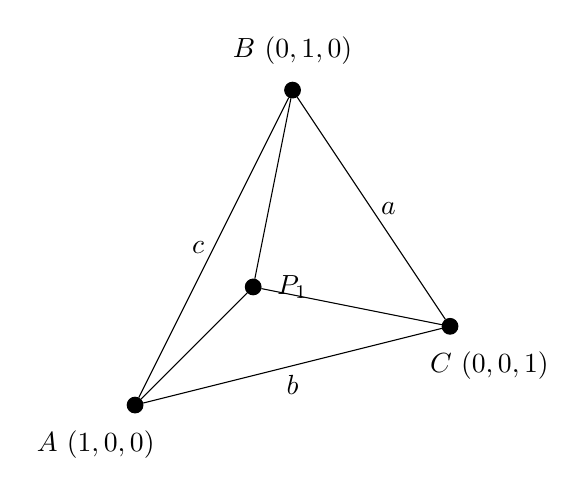
\begin{tikzpicture}
                        \node[rbtb] (a) at (0, 0) {};
                        \node[rbtb] (b) at (2, 4) {};
                        \node[rbtb] (c) at (4, 1) {};
                        \node[rbtb] (p1) at (1.5, 1.5) {};
                        \draw
                        (a) edge[left] node{$c$} (b)
                        (b) edge[right] node{$a$} (c)
                        (c) edge[below] node{$b$} (a);
                        \node at ($(a) + (-0.5, -0.5)$) {$A\ (1, 0, 0)$};
                        \node at ($(b) + (0, 0.5)$) {$B\ (0, 1, 0)$};
                        \node at ($(c) + (0.5, -0.5)$) {$C\ (0, 0, 1)$};
                        \node at ($(p1) + (0.5, 0)$) {$P_1$};
                        \draw
                        (p1) -- (a)
                        (p1) -- (b)
                        (p1) -- (c);
                    \end{tikzpicture}
                \end{center}
                This stems from the idea of the barycentre, being the centre of mass.
                However, we can use it to characterise any point on a plane with masses relative to a triangle.
                There are two degrees of freedom (note we can define the third point in terms of the first two, so long as they are not collinear).
            \subsubsection*{Points and Planes}
                We can use the vertices $\vec{a}$, $\vec{b}$, and $\vec{c}$ to specify points of a triangle; this can also be used to compute the edge vectors;
                \begin{center}
                    \begin{tikzpicture}
                        \node[rbtb] (a) at (0, 0) {};
                        \node[rbtb] (b) at (4, 1) {};
                        \node[rbtb] (c) at (2, 4) {};
                        \draw
                        (a) edge[->, left] node{$\vec{c} - \vec{a}$} (c)
                        (a) edge[->, below] node{$\vec{b} - \vec{a}$} (b);
                        \node at ($(a) + (-0.5, -0.5)$) {$\vec{a}$};
                        \node at ($(b) + (0.5, -0.5)$) {$\vec{b}$};
                        \node at ($(c) + (0, 0.5)$) {$\vec{c}$};
                    \end{tikzpicture}
                \end{center}
                Note that here we have two vectors $\vec{b} - \vec{a}$ and $\vec{c} - \vec{a}$, which form a basis for a plane; hence three non-collinear points determine a plane.
                This non-orthogonal basis can be used to specify the location of any point $\vec{p}$ on the plane (working with $(\beta, \gamma)$ coordinates, rather than $(x, y)$);
                $$\vec{p} = \vec{a} + \beta(\vec{b} - \vec{a}) + \gamma(\vec{c} - \vec{a})$$
                We can also reorder the equation as follows, to use $(\alpha, \beta, \gamma)$ as barycentric coordinates;
                \begin{align*}
                    \alpha & = 1 - \beta - \gamma \\
                    \vec{p} & = \vec{a} + \beta(\vec{b} - \vec{a}) + \gamma(\vec{c} - \vec{a}) \\
                    & = (1 - \beta - \gamma)\vec{a} + \beta\vec{b} + \gamma\vec{c} \\
                    & = \alpha\vec{a} + \beta\vec{b} + \gamma\vec{c}
                \end{align*}
                In \textbf{homogenous barycentric coordinates}, the sum $\alpha + \beta + \gamma$ is normalised to be the area of the triangle, whereas \textbf{areal coordinates / absolute barycentric coordinates} have the coordinates normalised by the area of the original triangle, such that $\alpha + \beta + \gamma = 1$ (this is what we assume).
                Therefore, we have the following rules;
                \begin{itemize}
                    \itemsep0em
                    \item \textbf{any point inside the triangle} \hfill $0 < \alpha, \beta, \gamma < 1$
                    \item \textbf{edge} \hfill one coefficient is 0
                    \item \textbf{vertex} \hfill two coefficients are 0, remaining must be 1
                \end{itemize}
                Note that a line $\beta = 0$ would go through $\vec{a}$ and $\vec{c}$, and a line $\beta = 1$ would go through $\vec{b}$ (and be parallel to the previous line).
                \medskip

                Recall that an implicit equation in 2D is defined as;
                $$f(x, y) = 0$$
                Where only points with $f(x, y) = 0$ are on a given line.
                The general implicit form is;
                $$Ax + By + C = 0$$
                And an implicit line through $(x_a, y_a)$ and $(x_b, y_b)$ is;
                $$(y_a - y_b)x + (x_b - x_a)y + x_ay_b - x_by_a = 0$$
                Therefore, given a triangle with vertices $(x_a, y_a)$, $(x_b, y_b)$ , and $(x_c, y_c)$, we have the following three line equations;
                \begin{align*}
                    f_{ab}(x, y) & = (y_a - y_b)x + (x_b - x_a)y + x_ay_b - x_by_a \\
                    f_{bc}(x, y) & = (y_b - y_c)x + (x_c - x_b)y + x_by_c - x_cy_b \\
                    f_{ca}(x, y) & = (y_c - y_a)x + (x_a - x_c)y + x_cy_a - x_ay_c
                \end{align*}
                Note that a barycentric coordinate such as $\beta$ is a \textbf{signed distance} from a line (in this case, the line through $\vec{a}$ and $\vec{c}$).
                We need to choose $k$ such that
                $$kf_{ac}(x, y) = \beta$$
                Since we know $\beta = 1$ at $\vec{b}$;
                $$kf_{ac}(x_a, y_b) = 1 \Leftrightarrow k = \frac{1}{f_{ac}(x_b, y_b)}$$
                Using this, we therefore have the barycentric coordinates for some arbitrary point $\vec{p}$ as;
                \begin{align*}
                    \alpha & = \frac{f_{bc}(x, y)}{f_{bc}(x_a, y_a)} \\
                    \beta & = \frac{f_{ac}(x, y)}{f_{ac}(x_b, y_b)} \\
                    \gamma & = 1 - \alpha - \beta
                \end{align*}
                In general, we can also define the barycentric area coordinates as the solution for the following linear system of equations;
                $$\begin{bmatrix}
                    x_a & x_b & x_c \\
                    y_a & y_b & y_c \\
                    1 & 1 & 1
                \end{bmatrix} \begin{bmatrix}
                    \alpha \\ \beta \\ \gamma
                \end{bmatrix} = \begin{bmatrix}
                    x \\ y \\ 1
                \end{bmatrix}$$
                We can convert from $(t_1, t_2, t_3)$ in trilinear coordinates to barycentric coordinates $(t_1a, t_2b, t_3c)$ (where we have the lengths of the sides).
                Similarly, conversion backwards would involve dividing through by $a$, $b$, and $c$.
            \subsubsection*{Triangle Rasterization}
                One method of generating fragments for a triangle is to check $(\alpha, \beta, \gamma)$.
                \begin{lstlisting}
                    for all x do
                      for all y do
                        compute (alpha, beta, gamma) for (x, y)
                        if (0 < alpha < 1 and
                            0 < beta  < 1 and
                            0 < gamma < 1) then
                          c = alpha c0 + beta c1 + gamma c2
                          draw pixel at (x, y) with colour c
                \end{lstlisting}
                It's important to note that we can also use the barycentric coordinates as weighting for colours; this can be done as we have normalised the coordinates.
                However in practice, this is done with optimised methods in the graphics hardware, including using fixed point precision (rather than floating-point), and done incrementally (withe the results from the previous pixel).
                Another optimisation is to take an axis aligned bounding box (by taking the minimum and maximum $x$ and $y$ coordinates).
            \subsubsection*{Visibility}
                While the above works fine for a single triangle, generally we have multiple triangles in our scene.
                Typically, we render the triangle closest to the camera, as that would be in front of the other triangles (there are exceptions such as transparency).
                \medskip

                Each pixel has a unique location in the framebuffer (image); however multiple fragments may be at the same address.
                Some approaches are as follows;
                \begin{itemize}
                    \itemsep0em
                    \item \textbf{painter's algorithm}
                        \smallskip

                        Here the triangles are sorted, using $z$ values in camera space.
                        The triangles are drawn from back to front (the highest $z$ value would be drawn first).
                        This not only suffers from efficiency issues due to the costly sorting, there are also issues with correctness.
                        These issues could arise from intersections of triangles, as well as cycles of overlap; this could be solved by splitting triangles (which is also expensive).
                    \item \textbf{depth buffer (z-buffer)}
                        \smallskip

                        In this solution, we keep a 2D buffer which has the same size as the image, initialised with some infinitely large number in each position.
                        When we render a fragment, we can also interpolate the $z$ value, and when each fragment is drawn we keep the one with the lowest $z$ value.
                        When a smaller value is encountered, the previous colour is overwritten.
                        \begin{lstlisting}
                            let CB be colour (frame) buffer
                            let ZB be z-buffer
                            initialise z-buffer contents to be 1.0 (far)
                            for each triangle T
                              rasterize T to generate fragments
                              for each fragment F with screen position (x, y, z) and colour C
                                if (z < ZB[x, y]) then
                                  update colour CB[x, y] = C
                                  update depth  ZB[x, y] = z
                        \end{lstlisting}
                        This method has multiple benefits, as it can handle intersections and cycles, as well as being simple to implement.
                        It can draw opaque polygons in any order.
                \end{itemize}
            \subsubsection*{Alias Effect}
                Rasterization can cause alias effects, where straight lines or triangle boundaries may look gagged.
                These are caused by undersampling, and can cause visual artefacts.
                Undersampling can be shown as follows;
                \begin{center}
                    \begin{tikzpicture}
                        \begin{scope}
                            \draw[fill=violet] (0, 0) -- (1, 0) -- (1, -1) -- (0, -1) -- cycle;
                            \draw[fill=teal] (1, 0) -- (2, 0) -- (2, -1) -- (1, -1) -- cycle;
                            \draw[fill=violet] (2, 0) -- (3, 0) -- (3, -1) -- (2, -1) -- cycle;
                            \draw[fill=teal] (3, 0) -- (4, 0) -- (4, -1) -- (3, -1) -- cycle;
                            \draw[fill=violet] (4, 0) -- (5, 0) -- (5, -1) -- (4, -1) -- cycle;
                            \draw[fill=teal] (5, 0) -- (6, 0) -- (6, -1) -- (5, -1) -- cycle;
                            \draw[very thick] (0, 0) -- (6, 0) -- (6, -1) -- (0, -1) -- cycle;
                            \foreach \x in {1,...,5} {
                                \draw[very thick] (\x, 0) -- (\x, -1);
                            }
                        \end{scope}
                        %inner sep=2pt, circle, draw=black, fill=black
                        \node at (-2, -1.5) {samples};
                        \node at (-2, -0.5) {texture};
                        \node at (11, -0.5) {\shortstack{appearance of textured\\polygon in the image}};
                        \node at (-2, -2.5) {$12$};
                        \begin{scope}[shift={(0, -2.5)}]
                            \node[inner sep=3pt, circle, draw=black, fill=violet] at (0.25, 0) {};
                            \node[inner sep=3pt, circle, draw=black, fill=violet] at (0.75, 0) {};
                            \node[inner sep=3pt, circle, draw=black, fill=teal] at (1.25, 0) {};
                            \node[inner sep=3pt, circle, draw=black, fill=teal] at (1.75, 0) {};
                            \node[inner sep=3pt, circle, draw=black, fill=violet] at (2.25, 0) {};
                            \node[inner sep=3pt, circle, draw=black, fill=violet] at (2.75, 0) {};
                            \node[inner sep=3pt, circle, draw=black, fill=teal] at (3.25, 0) {};
                            \node[inner sep=3pt, circle, draw=black, fill=teal] at (3.75, 0) {};
                            \node[inner sep=3pt, circle, draw=black, fill=violet] at (4.25, 0) {};
                            \node[inner sep=3pt, circle, draw=black, fill=violet] at (4.75, 0) {};
                            \node[inner sep=3pt, circle, draw=black, fill=teal] at (5.25, 0) {};
                            \node[inner sep=3pt, circle, draw=black, fill=teal] at (5.75, 0) {};
                        \end{scope}
                        \node at (-2, -3.5) {$6$};
                        \begin{scope}[shift={(0, -3.5)}]
                            \node[inner sep=3pt, circle, draw=black, fill=violet] at (0.25, 0) {};
                            \node[inner sep=3pt, circle, draw=black, fill=teal] at (1.25, 0) {};
                            \node[inner sep=3pt, circle, draw=black, fill=violet] at (2.25, 0) {};
                            \node[inner sep=3pt, circle, draw=black, fill=teal] at (3.25, 0) {};
                            \node[inner sep=3pt, circle, draw=black, fill=violet] at (4.25, 0) {};
                            \node[inner sep=3pt, circle, draw=black, fill=teal] at (5.25, 0) {};
                        \end{scope}
                        \node at (-2, -4.5) {$4$};
                        \begin{scope}[shift={(0, -4.5)}]
                            \node[inner sep=3pt, circle, draw=black, fill=violet] at (0.25, 0) {};
                            \node[inner sep=3pt, circle, draw=black, fill=teal] at (1.75, 0) {};
                            \node[inner sep=3pt, circle, draw=black, fill=teal] at (3.25, 0) {};
                            \node[inner sep=3pt, circle, draw=black, fill=violet] at (4.75, 0) {};
                        \end{scope}
                        \node at (-2, -5.5) {$3$};
                        \begin{scope}[shift={(0, -5.5)}]
                            \node[inner sep=3pt, circle, draw=black, fill=violet] at (0.25, 0) {};
                            \node[inner sep=3pt, circle, draw=black, fill=violet] at (2.25, 0) {};
                            \node[inner sep=3pt, circle, draw=black, fill=violet] at (4.25, 0) {};
                        \end{scope}
                        \foreach \x in {0,...,6} {
                            \draw[very thick, dashed] (\x, -1) -- (\x, -6);
                        }
                        \foreach \y in {0,...,4} {
                            \draw[very thick] (-3, -2 - \y) -- (6, -2 - \y);
                        }
                        \begin{scope}[shift={(0, 0)}]
                            \begin{scope}[shift={(8, -2)}]
                                \draw[fill=violet] (0, 0) -- (1, 0) -- (1, -1) -- (0, -1) -- cycle;
                                \draw[fill=teal] (1, 0) -- (2, 0) -- (2, -1) -- (1, -1) -- cycle;
                                \draw[fill=violet] (2, 0) -- (3, 0) -- (3, -1) -- (2, -1) -- cycle;
                                \draw[fill=teal] (3, 0) -- (4, 0) -- (4, -1) -- (3, -1) -- cycle;
                                \draw[fill=violet] (4, 0) -- (5, 0) -- (5, -1) -- (4, -1) -- cycle;
                                \draw[fill=teal] (5, 0) -- (6, 0) -- (6, -1) -- (5, -1) -- cycle;
                                \draw[very thick] (0, 0) -- (6, 0) -- (6, -1) -- (0, -1) -- cycle;
                                \foreach \x in {1,...,5} {
                                    \draw[very thick] (\x, 0) -- (\x, -1);
                                }
                            \end{scope}
                            \begin{scope}[shift={(8, -3)}]
                                \draw[fill=violet] (0, 0) -- (1, 0) -- (1, -1) -- (0, -1) -- cycle;
                                \draw[fill=teal] (1, 0) -- (2, 0) -- (2, -1) -- (1, -1) -- cycle;
                                \draw[fill=violet] (2, 0) -- (3, 0) -- (3, -1) -- (2, -1) -- cycle;
                                \draw[fill=teal] (3, 0) -- (4, 0) -- (4, -1) -- (3, -1) -- cycle;
                                \draw[fill=violet] (4, 0) -- (5, 0) -- (5, -1) -- (4, -1) -- cycle;
                                \draw[fill=teal] (5, 0) -- (6, 0) -- (6, -1) -- (5, -1) -- cycle;
                                \draw[very thick] (0, 0) -- (6, 0) -- (6, -1) -- (0, -1) -- cycle;
                                \foreach \x in {1,...,5} {
                                    \draw[very thick] (\x, 0) -- (\x, -1);
                                }
                            \end{scope}
                            \begin{scope}[shift={(8, -4)}]
                                \draw[fill=violet] (0, 0) -- (1, 0) -- (1, -1) -- (0, -1) -- cycle;
                                \draw[fill=teal] (1, 0) -- (2, 0) -- (2, -1) -- (1, -1) -- cycle;
                                \draw[fill=teal] (2, 0) -- (3, 0) -- (3, -1) -- (2, -1) -- cycle;
                                \draw[fill=teal] (3, 0) -- (4, 0) -- (4, -1) -- (3, -1) -- cycle;
                                \draw[fill=violet] (4, 0) -- (5, 0) -- (5, -1) -- (4, -1) -- cycle;
                                \draw[fill=teal] (5, 0) -- (6, 0) -- (6, -1) -- (5, -1) -- cycle;
                                \draw[very thick] (0, 0) -- (6, 0) -- (6, -1) -- (0, -1) -- cycle;
                                \foreach \x in {1,...,5} {
                                    \draw[very thick] (\x, 0) -- (\x, -1);
                                }
                            \end{scope}
                            \begin{scope}[shift={(8, -5)}]
                                \draw[fill=violet] (0, 0) -- (1, 0) -- (1, -1) -- (0, -1) -- cycle;
                                \draw[fill=violet] (1, 0) -- (2, 0) -- (2, -1) -- (1, -1) -- cycle;
                                \draw[fill=violet] (2, 0) -- (3, 0) -- (3, -1) -- (2, -1) -- cycle;
                                \draw[fill=violet] (3, 0) -- (4, 0) -- (4, -1) -- (3, -1) -- cycle;
                                \draw[fill=violet] (4, 0) -- (5, 0) -- (5, -1) -- (4, -1) -- cycle;
                                \draw[fill=violet] (5, 0) -- (6, 0) -- (6, -1) -- (5, -1) -- cycle;
                                \draw[very thick] (0, 0) -- (6, 0) -- (6, -1) -- (0, -1) -- cycle;
                                \foreach \x in {1,...,5} {
                                    \draw[very thick] (\x, 0) -- (\x, -1);
                                }
                            \end{scope}
                        \end{scope}
                    \end{tikzpicture}
                \end{center}
                The general solution is to apply some blurring to the boundary, to reduce the effect.
                The most successful technique is to perform \textbf{supersampling}, which is then downsampled to the resolution of the screen.
                A local average can cause undesirable effects, therefore a weighted average is normally taken, such as the following (allowing us to sample from the texels adjacent, like in computer games);
                $$\frac{1}{36}\begin{bmatrix}
                    1 & 4 & 1 \\
                    4 & 16 & 4 \\
                    1 & 4 & 1
                \end{bmatrix}$$
        \subsection*{Lecture 10 - Ray Tracing I}
            From here we look at a different method of generating images.
            Note that before we were unable to create infinitely reflecting surfaces, nor did we cover how to create shadows (which is an important depth cue) - including self shadowing.
            We were also unable to create distortions in reflective geometry or refraction.
            \subsubsection*{Illumination}
                Note that we've only covered the \textbf{direct} illumination (which can be done easily with the Phong model).
                In direct illumination, a point receives light \textbf{directly} from all light sources in the scene.
                On the other hand, in \textbf{global} illumination, a point only receives light after \textbf{interacting} with other objects in the scene.
                As such, points might be in shadow or rays may be refracted through transparent material.
            \subsubsection*{Ray Casting}
                A technique developed for pen-plotter in 1968 was to cast a ray per pixel (\textbf{from} the viewpoint outwards).
                If the ray from the viewpoint hits an object, that point is traced to the light source; if it doesn't intersect with anything else, the global illumination model is applied.
                However, if it intersects another object, it is not drawn (or filled in black).
                While the algorithm is quite simple, this is computationally expensive.
                \begin{lstlisting}
                    trace ray
                      intersect all objects
                      colour = ambient term
                      for every light cast shadow ray
                        colour += local shading term # add local shading term if light is not occluded
                \end{lstlisting}
                Turner Whitted took the concept further, evaluating not only shadows, but also reflections, refractions, and other effects.
                Note that casting a ray is simply a point plus a direction.
                At each intersection, if the surface is reflective, we can also cast another ray.
                If the surface is transparent, we can also attempt to perform refraction.
                This was the first global illumination mode; an object's colour is influenced by lights and other objects in the scene, and can simulate real lighting effects such as specular reflection and refractive transmission.
                \begin{center}
                    See slide 9 for a diagram
                \end{center}
                The algorithm is simple, but gives way for a recursive algorithm (note we can stop this at some arbitrary point);
                \begin{lstlisting}
                    trace ray
                      intersect all objects
                      colour = ambient term
                      for every light cast shadow ray
                        colour += local shading term # add local shading term if light is not occluded
                      if mirror
                        colour += k_refl * trace reflected ray
                      if transparent
                        colour += k_trans * trace transmitted ray
                \end{lstlisting}
                We can either stop after some recursion depth (after some number of bounces), or we can stop once the ray contribution (from the reflected / transmitted rays) become too small.
                \medskip

                We have the following types of rays;
                \begin{itemize}
                    \itemsep0em
                    \item \textbf{primary (viewing) rays}
                        \smallskip

                        These are rays cast from the viewpoint to the nearest intersection.
                        Local illumination is computed according to the Phong model;
                        $$L = k_a + (k_d (\vec{n \cdot \vec{l}}) + k_s (\vec{v} \cdot \vec{r})^q)I_s$$
                    \item \textbf{secondary rays}
                        \smallskip

                        Secondary rays are any other rays (that aren't \red{primary rays}) - rays originating at intersection points, and can be caused by a number of things;
                        \begin{itemize}
                            \itemsep0em
                            \item \violet{reflected ray}
                                \smallskip

                                This computes the mirror contribution, by casting a ray in the direction symmetric with respect to the surface normal, and multiply by the reflection coefficient.
                                The direction of the ray is calculated in the same way as the ideal reflection ray (from the specular component), or can be worked out as follows, where $\vec{v^\prime}$ is the direction of the secondary ray, $\vec{v}$ is the primary ray, and $\vec{n}$ is the unit surface normal;
                                $$\vec{v^\prime} = \vec{v} - (2\vec{v} \cdot \vec{n})\vec{n}$$
                            \item \teal{shadow ray}
                                \smallskip

                                Shadows can be added as follows, where we omit the diffuse and specular if the light source is obscured (hard shadows);
                                \begin{align*}
                                    L & = k_a + s(k_d(\vec{n} \cdot \vec{l}) + k_s(\vec{v} \cdot \vec{r})^q)I_s + k_\text{reflected}L_\text{reflected} + k_\text{refracted}L_\text{refracted} \\
                                    s & = \begin{cases}
                                        0 & \text{if light source obscured} \\
                                        1 & \text{if light source not obscured}
                                    \end{cases}
                                \end{align*}
                                However, we can use multiple shadow rays to sample an area light source, allowing us to create soft shadows.
                            \item \blue{transmitted (refracted) ray}
                                \smallskip

                                The angle of the refracted ray is determined by Snell's law;
                                $$\eta_1\sin(\phi_1) = \eta_2\sin(\phi_2)$$
                                Note that $\eta_1$ and $\eta_2$ are constants for mediums 1 and 2, respectively.
                                Similarly, $\phi_1$ and $\phi_2$ are angles between the respective rays and the surface normal.
                                \begin{center}
                                    \begin{tikzpicture}
                                        \draw[fill=black!20, black!20] (-1.25, 0) -- (1.25, 0) -- (1.25, -1.25) -- (-1.25, -1.25) -- cycle;
                                        \draw (-1.25, 0) -- (1.25, 0);
                                        \draw (0, -1) edge[dashed, ->] (0, 1);
                                        \node at (0, 1.25) {$\vec{n}$};
                                        \draw (-1, 1) edge[->, left] node{$\vec{v}$} (0, 0);
                                        \draw (0, 0) edge[->, right] node{$\vec{v^\prime}$} (0.5, -1);
                                        \draw (0, 0) ++(90:0.5) arc (90:135:0.5);
                                        \draw (0, 0) ++(270:0.5) arc (270:296.6:0.5);
                                        \node at (0.4, 0.3) {$\phi_1$};
                                        \node at (-0.4, -0.3) {$\phi_2$};
                                    \end{tikzpicture}
                                \end{center}
                                Snell's law can also be written as the following, in vector notation;
                                $$k_1(\vec{v} \cdot \vec{n}) = k_2(\vec{v^\prime} \cdot \vec{n})$$
                                The direction of the refracted ray can be written as;
                                $$\vec{v^\prime} = \frac{\eta_1}{\eta_2}\left(\left(\sqrt{(\vec{n} \cdot \vec{v})^2 + \left(\frac{\eta_2}{\eta_1}\right)^2 - 1} - \vec{n} \cdot \vec{v}\right) \vec{n} + \vec{v}\right)$$
                                It's important to note that the above only has a solution given the following condition;
                                $$(\vec{n} \cdot \vec{v})^2 > 1 - \left(\frac{\eta_2}{\eta_1}\right)^2$$
                                If the angle of the refracted ray is larger than $90^\circ$ (due to a large incident ray), the ray becomes reflected rather than refracted (total internal reflection).
                                \medskip

                                In the stack based implementation, we will also need to keep track of the material ($\eta$), and whether we are entering or leaving.
                        \end{itemize}
                \end{itemize}
                This allows us to express illumination as the following;
                $$L = k_a + (k_d (\vec{n \cdot \vec{l}}) + k_s (\vec{v} \cdot \vec{r})^q)I_s + \underbrace{k_\text{reflected}L_\text{reflected} + k_\text{refracted}L_\text{refracted}}_\text{recursion}$$
                Note that the grey circles below denote \textbf{opaque} surfaces, and the red dot denotes a light source.
                \begin{center}
                    \begin{tikzpicture}
                        \node[rbtb] (vp) at (0, 0) {};
                        \node[rbtr] (light) at (1, 2) {};
                        \draw (0.707, 4) circle (1);
                        \draw[fill=black!20] (-4, 2.586) circle (1);
                        \draw[fill=black!20] (-1, 2.5) circle (0.5);

                        \draw
                        (vp) edge[red, ->] (0, 3.293)
                        (0, 3.293) edge[teal, ->, below] node{$L_1$} (light)
                        (0, 3.293) edge[blue, ->, left] node{$T_1$} (0.707, 5)
                        (0.707, 5) edge[blue, ->, above] node{$T_3$} (2, 6)
                        (0.707, 5) edge[teal, ->, left] node{$L_3$} (light)
                        (0.707, 5) edge[violet, ->, right] node{$R_3$} (1.414, 3.293)
                        (0, 3.293) edge[violet, ->, above] node{$R_1$} (-3.293, 3.293)
                        (-3.293, 3.293) edge[violet, ->, left] node{$R_2$} (-3.293, 5)
                        (-3.293, 3.293) edge[teal, ->, below] node{$L_2$} (-1.441, 2.735);
                    \end{tikzpicture}
                \end{center}
                Since we cannot perform recursion in GLSL, this should be done iteratively (which can be done for the reflections, refraction would require state to be stored).
            \subsubsection*{Precision Problems}
                However; while this will work completely fine in practice (as well as the majority of the time), consider the case where we have a sphere and a ray.
                Due to rounding errors, the intersection point between these two may end up \textbf{inside} inside the sphere (beneath the surface), and when we cast the shadow ray from the intersection point, it will end up intersecting with itself again, hence leading to unwanted self occlusion (note that the dashed lines represent the issue caused by the rounding error, and the solid lines represent the desired effect) - the effect is obviously exaggerated here;
                \begin{center}
                    \begin{tikzpicture}
                        \node[rbtb] (vp) at (0, 0) {};
                        \node[rbtr] (light) at (2, 1) {};
                        \draw
                        (4, 0) circle (1)
                        (vp) edge[->] (3, 0)
                        (3, 0) edge[->] (light)
                        (vp) edge[->, dashed] (3.5, 0)
                        (3.5, 0) edge[->, dashed] (3.047, 0.302);
                    \end{tikzpicture}
                \end{center}
                As such, we can assign some $\varepsilon$ value; if the length of the shadow ray ($\mu$) is smaller than some $\varepsilon$, we assume it is on the surface, and shift the ray slightly in the required direction (along the surface normal) for it to be outside of the object.
            \subsubsection*{Fresnel Factor}
                Traditional ray tracing has a constant coefficient for reflection.
                A better approach is to mix the reflected and refracted light according to the Fresnel factor;
                $$L = k_\text{fresnel}L_\text{reflected} - (1 - k_\text{fresnel})L_\text{refracted}$$
                Schlick's approximation does the following;
                $$k_\text{fresnel}(\theta) = k_\text{fresnel}(0) + (1 - k_\text{fresnel}(0))(1 - (\vec{n} \cdot \vec{l}))^5$$
                Setting $k_\text{fresnel}(0) = 0.8$ gives a surface like stainless steel, apparently.
            \subsubsection*{Monte-Carlo}
                A more computationally expensive approach which simulates the randomness of real light better is to cast multiple random rays from an intersection point (recursively).
                At some point, all of the intersection points are sent to the light source as before.
                On the other hand, Monte-Carlo path tracing only traces one secondary ray per recursion, but will send many primary rays per pixel.
        \subsection*{Lecture 11 - Ray Tracing II}
            \subsubsection*{Calculating Intersections}
                For each ray, we need to find the nearest intersection point, and calculate all possible intersections with each object inside the viewing volume.
                Our scene can be defined with solid models (such as spheres and cylinders), as well as surface models (such as planes, triangles, and polygons).
                In general, anything that can be parameterised can be rendered with ray tracing.
                \medskip

                Rays are parametric lines, defined as an origin $\vec{p_0}$ and a direction $\vec{d}$;
                $$\vec{p}(\mu) = \vec{p_0} + \mu\vec{d}$$
                For a ray, we can determine $\vec{d}$ as follows, where we have the position of the pixel on the viewing plane $\vec{p_0}$ and the position of the viewpoint $\vec{p_v}$;
                $$\vec{d} = \frac{\vec{p_0} - \vec{p_v}}{| \vec{p_0} - \vec{p_v} |}$$
                Since the viewing ray is parameterised by $\mu$, $\mu > 0$ denotes the part of the ray \textbf{behind} the viewing plane, and $\mu < 0$ denotes the part of the ray in \textbf{front} of the viewing plane.
                \medskip

                Consider a sphere, where any point on the surface $\vec{d}$ will satisfy the following (where $r$ is the radius and $\vec{p_s}$ is the position in world space);
                $$|\vec{q} - \vec{p_s}|^2 - r^2 = 0$$
                Assuming that our viewing ray will intersect the sphere, we can substitute $\vec{q}$ with the line equation;
                $$|\vec{p_0} + \mu\vec{d} - \vec{p_s}|^2 - r^2 = 0$$
                If we allow $\Delta\vec{p} = \vec{p_0} - \vec{p_s}$ (and expand the dot product), we obtain the following quadratic equation (and corresponding solution);
                $$\mu^2 + 2\mu(\vec{d} \cdot \Delta\vec{p}) + |\Delta\vec{p}|^2 - r^2 = 0 \Rightarrow \mu = -\vec{d} \cdot \Delta\vec{p} \pm \sqrt{\violet{(\vec{d} \cdot \Delta\vec{p})^2 - |\Delta\vec{p}|^2 + r^2}}$$
                This gives us two solutions (since the ray would pass through the object) - in the case of solid objects, we want the one that's closer (hence the smaller $\mu$).
                If the ray does not intersect, there will be no solution (negative under the square root; \violet{discriminant}) - if this is the case, we want to stop in order to save computation.
                Once we have a value for $\mu$, we can plug it back into the line equation to obtain the position.
                \medskip

                A cylinder can be described by two position vectors ($\vec{p_1}$ and $\vec{p_2}$), describing the first and second end points of the long axis of the cylinder, and a radius $r$.
                The axis can be written as $\Delta\vec{p} = \vec{p_1} - \vec{p_2}$, and parameterised by $\alpha \in [0, 1]$.
                We can solve the following equation to obtain an intersection with the ray - note that $\vec{q}$ denotes a normal from the axis vector to the surface;
                $$\vec{p_1} + \alpha\Delta\vec{p} + \vec{q} = \vec{p_0} + \mu\vec{d}$$
                However, since we know $\vec{q} \cdot \Delta\vec{p} = 0$ (since it is a normal), we have;
                $$\alpha(\Delta\vec{p} \cdot \Delta\vec{p}) = \vec{p_0} \cdot \Delta\vec{p} + \mu\vec{d} \cdot \Delta\vec{p} - \vec{p_1} \cdot \Delta\vec{p}$$
                Solving for $\alpha$ gives the following result;
                $$\alpha = \frac{\vec{p_0} \cdot \Delta\vec{p} + \mu\vec{d} \cdot \Delta\vec{p} - \vec{p_1} \cdot \Delta\vec{p}}{\Delta\vec{p} \cdot \Delta\vec{p}}$$
                This can be substituted back into the equation to obtain;
                $$\vec{q} = \vec{p_0} + \mu\vec{d} - \vec{p_1} - \left(\frac{\vec{p_0} \cdot \Delta\vec{p} + \mu\vec{d} \cdot \Delta\vec{p} - \vec{p_1} \cdot \Delta\vec{p}}{\Delta\vec{p} \cdot \Delta\vec{p}}\right) \Delta\vec{p}$$
                Since we have $\vec{q} \cdot \vec{q} = r^2$, we can use the same approach for the quadratic equation for $\mu$;
                $$r^2 = \left(\vec{p_0} + \mu\vec{d} - \vec{p_1} - \left(\frac{\vec{p_0} \cdot \Delta\vec{p} + \mu\vec{d} \cdot \Delta\vec{p} - \vec{p_1} \cdot \Delta\vec{p}}{\Delta\vec{p} \cdot \Delta\vec{p}}\right) \Delta\vec{p}\right)^2$$
                If this gives two solutions, $\mu_1, \mu_2$, there is an intersection, otherwise there is no intersection.
                Assuming that $\mu_1 < \mu_2$, we obtain the two following solutions;
                \begin{align*}
                    \alpha_1 & = \frac{\vec{p_0} \cdot \Delta\vec{p} + \mu_1\vec{d} \cdot \Delta\vec{p} - \vec{p_1} \cdot \Delta\vec{p}}{\Delta\vec{p} \cdot \Delta\vec{p}} \\
                    \alpha_2 & = \frac{\vec{p_0} \cdot \Delta\vec{p} + \mu_2\vec{d} \cdot \Delta\vec{p} - \vec{p_1} \cdot \Delta\vec{p}}{\Delta\vec{p} \cdot \Delta\vec{p}}
                \end{align*}
                If $\alpha_1 \in (0, 1)$, then the intersection is on the outside surface, whereas if $\alpha_2 \in (0, 1)$, the intersection is on the inside surface.
                If we only have one of these $\alpha$s, we may have to intersect with some disc at the top or bottom of the cylinder.
                \medskip

                We can intersect a ray with a plane using the following (where $\vec{p_1}$ is a point on the plane, and $\vec{q}$ is a vector from the point on the plane to the intersection point);
                $$\vec{p_1} + \vec{q} = \vec{p_0} + \mu$$
                Since $\vec{q}$ would be perpendicular to the plane's normal $\vec{n}$, we can subtract $\vec{p_1}$ and multiply by the normal to obtain $\mu$;
                $$\vec{q} \cdot \vec{n} = 0 = (\vec{p_0} - \vec{p_1}) \cdot \vec{n} + \mu\vec{d} \cdot \vec{n} \Rightarrow \mu = -\frac{(\vec{p_0} - \vec{p_1}) \cdot \vec{n}}{\vec{d} \cdot \vec{n}}$$
                Note that a triangle is a smaller part of a plane;
                \begin{center}
                    \begin{tikzpicture}
                        \draw[very thick, fill=black!20] (-1, 0) -- (4, 0) -- (4, -3) -- (-1, -3) -- cycle;
                        \coordinate (p1) at (2.5, -2.5);
                        \coordinate (p2) at (0.5, -2.5);
                        \coordinate (p3) at (1.5, -0.5);
                        \draw[white, fill=white] (p1) -- (p2) -- (p3) -- (p1);
                        \draw
                        (p1) edge[very thick, -latex, below] node{$\vec{a}$} (p2)
                        (p1) edge[very thick, -latex, right] node{$\vec{b}$} (p3)
                        (p2) edge[very thick, dashed] (p3);
                        \node at ($(p1) + (0.5, 0)$) {$\vec{p_1}$};
                        \node at ($(p2) + (-0.5, 0)$) {$\vec{p_2}$};
                        \node at ($(p3) + (-0.5, 0)$) {$\vec{p_3}$};
                    \end{tikzpicture}
                \end{center}
                In order to calculate intersections for triangles, we need to test if the triangle is \textbf{front facing} ($\vec{d} \cdot \vec{n} < 0$), and whether the ray intersects the plane of the triangle (as before).
                We also need to test whether the intersection point is \textbf{inside} the triangle.
                \begin{align*}
                    \vec{a} & = \vec{p_2} - \vec{p_1} \\
                    \vec{b} & = \vec{p_3} - \vec{p_1} \\
                    \vec{n} & = \vec{a} \times \vec{b} & \text{normal of plane} \\
                    \vec{q} & = \alpha\vec{a} + \beta\vec{b} & \text{test intersection point inside triangle}
                \end{align*}
                We know that a point is inside the triangle if the all of the following three hold;
                \begin{itemize}
                    \itemsep0em
                    \item $0 \leq \alpha \leq 1$
                    \item $0 \leq \beta \leq 1$
                    \item $\alpha + \beta \leq 1$
                \end{itemize}
                $\alpha$ and $\beta$ can be calculated as follows;
                \begin{align*}
                    \alpha & = \frac{(\vec{b} \cdot \vec{b})(\vec{q} \cdot \vec{a}) - (\vec{a} \cdot \vec{b})(\vec{q} \cdot \vec{b})}{(\vec{a} \cdot \vec{a})(\vec{b} \cdot \vec{b})^2 - (\vec{a} \cdot \vec{b})^2} \\
                    \beta & = \frac{\vec{q} \cdot \vec{b} - \alpha(\vec{a} \cdot \vec{b})}{\vec{b} \cdot \vec{b}}
                \end{align*}
                A more efficient implementation of this concept is to translate the origin of the ray, and change the base of the vector yielding parameter vector $(t, u, v) \equiv (\mu, \alpha, \beta)$ - here we have $t$ being the distance to the plane in which the triangle lies and $(u, v)$ being the barycentric coordinates inside the triangle.
                The plane equation doesn't need to be computed on the fly (as we have done previously).
                \begin{lstlisting}
                    // v1,v2,v3 are triangle vertices,
                    // origin denotes the ray origin
                    bool triangle_intersection(vec3 v1, vec3 v2, vec3 v3, vec3 origin, vec3 ray_dir, float* out) {
                        vec3 edge1 = v2 - v1;
                        vec3 edge2 = v3 - v1;

                        // begin determinant calculation, also used for u
                        vec3 p = cross(ray_dir, edge2);

                        // if det is near 0, ray is parallel to (or in) plane
                        float det = dot(edge1, p);
                        if (det > -EPSILON && det < EPSILON) {
                            return false;
                        }

                        float inv_det = 1.0f / det;

                        // distance from v1 to ray origin
                        vec3 t = origin - v1;

                        // calculate u and test bound
                        float u = dot(t, p) * inv_det;

                        // intersection out of triangle
                        if (u < 0.0f || u > 1.0f) {
                            return false;
                        }

                        // prepare to test v parameter
                        vec3 q = cross(t, edge1);
                        float v = dot(ray_dir, q) * inv_det;

                        // intersection out of triangle
                        if (v < 0.0f || v > 1.0f) {
                            return false;
                        }

                        float mu = dot(edge2, q) * inv_det;
                        if (t > EPSILON) {
                            *out = mu;
                            return true;
                        }
                    }
                \end{lstlisting}
            \subsubsection*{Performance}
                The core algorithm is easy to implement, and extends well to global illumination (including shadows, reflection / refraction, multiple bounces, and atmospheric effects).
                However, there is a significant performance cost, as it takes multiple seconds per frame, rather than generating multiple frames per second.
                \medskip

                In order to improve performance, we can reduce the number of bounces (however this may lead to less realistic lighting), and in generally we can reduce the number of rays.
                If we are rendering an object in a generally empty scene, we are wasting many rays that will never intersect.
                This can be accelerated by implementing an axis aligned bounding box for the object; where we discard any rays that don't intersect the box.
                \medskip

                We can use the projection matrix to project the box, allowing us to immediately know which pixels will be inside the box (and which won't).
                Most complicated effects are implemented using multi-pass, or to use parts of the pipeline.
                \medskip

                Another approach is to use a \textbf{regular grid}, where we divide the world into a grid, and at each region we store pointers to the objects that are in the region.
                A ray is shot through the space and only objects in the regions it passes are checked.
                This technique is rarely used.
                Instead, adaptive grids are use, which subdivide the world until each cell contains no more than $n$ elements (or some maximum depth $d$ has been reached).
                This would be done in world space (rather than screen space), as this computation is expensive; we would rather do it once than to do it on every change of the camera position.
                \medskip

                Another approach is to create a \textbf{binary space partition (BSP) tree}, where the space is recursively partitioned by planes.
                Each cell is a convex polyhedron.
                Rays can be traced by recursion on the tree, and the construction enables a simple front-to-back traversal.
        \subsection*{Lecture 12 - Splines I}
            We can either think of splines as interpolating splines (defined by a start point, an end point, and a small set of points called \textbf{knots} or \textbf{control points} that they go through smoothly), or approximating splines which have the same points, but \textbf{don't need to pass through} these points.
            Both will go through the start and end point.
            \medskip

            The simplest splines are equations in $x$ and $y$ (we are staying within 2D for now).
            With three points, we can calculate $a_2, a_1, a_0$ for the polynomial spline;
            $$y = a_2x^2 + a_1x + a_0$$
            Only one curve will fit the data.
            An issue with this method is that we cannot define splines where the resulting function would have two $y$ values for the same $x$.
            \subsubsection*{Paramterisation}
                Paramterisation involves a set of points and a set of parameters that scale some properties of a function.
                We can write the spline in a vector form, with some parameter $\mu$ from 0 to 1;
                $$\vec{P} = \vec{a_2}\mu^2 + \vec{a_1}\mu + \vec{a_0}$$
                As before, we set up observations, and solve for the unknowns.
                A trivial case would be $\mu = 0$, at the start of the curve, hence;
                $$\vec{P_0} = \vec{a_2}0^2 + \vec{a_1}0 + \vec{a_0} \Rightarrow \vec{a_0} = \vec{P_0}$$
                Suppose the spline ends at $\vec{P_2}$, at which point we have $\mu = 1$, and at $\mu = \frac{1}{2}$ it passes through $\vec{P_1}$;
                \begin{align*}
                    \vec{P_2} & = \vec{a_2}\mu^2 + \vec{a_1}\mu + \vec{a_0} \\
                    & = \vec{a_2} + \vec{a_1} + \vec{a_0} \\
                    & = \vec{a_2} + \vec{a_1} + \vec{P_0} \\
                    \vec{P_1} & = \vec{a_2}\mu^2 + \vec{a_1}\mu + \vec{a_0} \\
                    & = \frac{1}{4}\vec{a_2} + \frac{1}{2}\vec{a_1} + \vec{P_0}
                \end{align*}
                Note that this process works in however many dimensions we are working in.
                Also note that there are many possibilities for what the spline could be fitted to (with the same points) depending on the $\mu$ values we give to each of the points.
                \medskip

                In general, these parametric polynomial splines have an order to match the number of control points; 3 control points leads to a quadratic, 4 control points leads to a cubic, and so on.
                Higher order polynomials tend to be undesirable as they can overfit and oscillate.
            \subsubsection*{Spline Patches}
                To avoid the problem of oscillation, we can use spline patches, where splines are pieced together, each patch starting from the end of the previous patch.
                The simplest (and most effective) way to calculate parametric spline patches is to use a cubic polynomial (which also tends to look natural).
                The patch of the spline between $\vec{P_1}$ and $\vec{P_2}$ is given by;
                $$\vec{P} = \vec{a_3}\mu^3 + \vec{a_2}\mu^2 + \vec{a_1}\mu + \vec{a_0}$$
                \begin{center}
                    \begin{tikzpicture}
                        \begin{axis}[
                            xticklabels={,,},
                            yticklabels={,,},
                            axis on top=true,
                            axis line style=thick,
                            samples=90
                        ]
                            \addplot[very thick, patch, patch type=cubic spline, black] coordinates {
                                (0, 0)
                                (8, 3)
                                (3, 1.75)
                                (5, 1.25)
                            };
                            \node[label={0:{$\vec{P_0}$}}, circle, fill=black, inner sep=2pt] at (axis cs:0,0) {};
                            \node[label={270:{$\vec{P_1}$}}, circle, fill=black, inner sep=2pt] at (axis cs:3,1.75) {};
                            \node[label={270:{$\vec{P_2}$}}, circle, fill=black, inner sep=2pt] at (axis cs:5,1.25) {};
                            \node[label={180:{$\vec{P_3}$}}, circle, fill=black, inner sep=2pt] at (axis cs:8,3) {};
                        \end{axis}
                    \end{tikzpicture}
                \end{center}
                Note that we want also want the connection between patches to be \textbf{smooth} - the gradients must match when two patches meet.
                We can get the gradient at the points $\vec{P_1}$ and $\vec{P_2}$ (denote it as $\vec{P_1^\prime}$ and $\vec{P_2^\prime}$ respectively) as follows;
                \begin{align*}
                    \vec{P_1^\prime} & = \frac{1}{2} (\vec{P_2} - \vec{P_0}) \\
                    \vec{P_2^\prime} & = \frac{1}{2} (\vec{P_3} - \vec{P_1})
                \end{align*}
                To calculate a spline patch joining $\vec{P_i}$ and $\vec{P_{i + 1}}$, we can do the following;
                \begin{align*}
                    \vec{P} & = \vec{a_3}\mu^3 + \vec{a_2}\mu^2 + \vec{a_1}\mu + \vec{a_0} \\
                    \mu & = 0 & \text{at $\vec{P_i}$} \\
                    \mu & = 1 & \text{at $\vec{P_{i + 1}}$} \\
                    \vec{P_i} & = \vec{a_0} & \text{substituting values} \\
                    \vec{P_{i + 1}} & = \vec{a_3} + \vec{a_2} + \vec{a_1} + \vec{a_0} \\
                    \vec{P^\prime} & = 3\vec{a_3}\mu^2 + 2\vec{a_2}\mu + \vec{a_1} & \text{differentiating with respect to $\mu$} \\
                    \vec{P_i^\prime} & = \vec{a_1} & \text{substituting $\mu$} \\
                    \vec{P_{i + 1}^\prime} & = 3\vec{a_3} + 2\vec{a_2} + \vec{a_1}
                \end{align*}
                These four equations can then be put into matrix form as follows;
                $$\begin{bmatrix}
                    1 & 0 & 0 & 0 \\
                    0 & 1 & 0 & 0 \\
                    1 & 1 & 1 & 1 \\
                    0 & 1 & 2 & 3
                \end{bmatrix} \begin{bmatrix}
                    \vec{a_0} \\
                    \vec{a_1} \\
                    \vec{a_2} \\
                    \vec{a_3}
                \end{bmatrix} = \begin{bmatrix}
                    \vec{P_i} \\
                    \vec{P_i^\prime} \\
                    \vec{P_{i + 1}} \\
                    \vec{P_{i + 1}^\prime}
                \end{bmatrix}$$
                Since the initial matrix is always the same, whether in 2D or 3D, and is well defined, we can just invert the matrix as follows, which is the same for every patch;
                $$\begin{bmatrix}
                    \vec{a_0} \\
                    \vec{a_1} \\
                    \vec{a_2} \\
                    \vec{a_3}
                \end{bmatrix} = \begin{bmatrix}
                    1 & 0 & 0 & 0 \\
                    0 & 1 & 0 & 0 \\
                    -3 & -2 & 3 & -1 \\
                    2 & 1 & -2 & 1
                \end{bmatrix} \begin{bmatrix}
                    \vec{P_i} \\
                    \vec{P_i^\prime} \\
                    \vec{P_{i + 1}} \\
                    \vec{P_{i + 1}^\prime}
                \end{bmatrix}$$
            \subsubsection*{Smoothness}
                Note a parametric curve is defined as the following (in 2D);
                $$\vec{P}(\mu) = \begin{bmatrix}
                    x(\mu) \\
                    y(\mu)
                \end{bmatrix}$$
                We can use the following definitions for parametric continuity (where we look at the curve as a function rather than a shape) - note that the agreement happens at the junction between the two curves;
                \begin{itemize}
                    \itemsep0em
                    \item $C^0$ continuous \hfill $(x, y)$ values of the curve agree
                    \item $C^1$ continuous (what we just did) \hfill both $(x, y)$ values and first derivatives of the curve agree
                    \item $C^2$ continuous \hfill $(x, y)$ values, as well as first \textbf{and} second parametric derivatives all agree
                    \item $G^1$ continuous
                        \smallskip

                        This is geometric continuity (note that $G^0$ is equivalent to $C^0$), where it is defined only with the shape of the curve.
                        Here the first derivatives are proportional (hence the tangent vectors are parallel) at the junction.
                        Note that the $(x, y)$ values must still agree.
                        Higher order geometric continuity can be difficult to define.
                \end{itemize}
            \subsubsection*{Bezier Curves}
                The main characteristics are that the end points are interpolated, and the slope at the end is the same as the line joining the end point to its neighbour.
                A typical Bezier curve looks like the following;
                \begin{center}
                    \begin{tikzpicture}
                        \node[rbtb] (p0) at (0, 0) {};
                        \node[rbtb] (p1) at (1, 4) {};
                        \node[rbtb] (p2) at (4, 4.5) {};
                        \node[rbtb] (p3) at (3, 1) {};
                        \draw[very thick]
                        (p0) .. controls (p1) and (p2) .. (p3)
                        (p0) edge[dotted] (p1)
                        (p1) edge[dotted] (p2)
                        (p2) edge[dotted] (p3);
                        \node at ($(p0) + (-0.5, 0)$) {$\vec{P_0}$};
                        \node at ($(p1) + (-0.5, 0)$) {$\vec{P_1}$};
                        \node at ($(p2) + (0.5, 0)$) {$\vec{P_2}$};
                        \node at ($(p3) + (0.5, 0)$) {$\vec{P_3}$};
                    \end{tikzpicture}
                \end{center}
                Paul de Casteljau's algorithm describes a geometric construction for computing and visualising a Bezier curve.
                Similar to a cubic path, the parameter $\mu$ is 0 at the start of the curve, and 1 at the end.
                This construction is recursive and made can be made for any value of $\mu$.
                Drawing it is quite difficult (in TikZ), so just read the slides.
            \subsubsection*{Bernstein Blending Function}
                Splines (including Bezier curves) can be formulated as a blend of the control points.
                The following vector line equation is a linear blend of two points (could be considered a two-point Bezier curve);
                $$\vec{P} = (1 - \mu)\vec{P_0} + \mu\vec{P_1}$$
                For $N + 1$ control points, we have the following;
                \begin{align*}
                    \vec{P}(\mu) & = \summation{i = 1}{N} W(N, i, \mu) \vec{P_i} \\
                    W(N, i, \mu) & = {N \choose i} \mu^i (1 - \mu)^{N - i} & \text{Bernstein blending function}\\
                    {N \choose i} & = \frac{N!}{(N - i)!i!}
                \end{align*}
                Note that with $N = 3$ (4 points), it expands to a cubic polynomial.
        \subsection*{Lecture 13 - Splines II}
            \subsubsection*{Non-Parametric Surfaces}
                A non-parametric surface can be constructed from Cartesian equations directly, for example, given a certain $x, z$ coordinate, we can determine a $y$ coordinate.
                These have the same problems as non-parametric splines.
                \medskip

                Since there are 9 scalar unknowns (due to symmetry) in the following, we need to specify 9 points in which the surface needs to pass through;
                $$\begin{bmatrix}
                    x & y & z & 1
                \end{bmatrix} \begin{bmatrix}
                    a & b & c & d \\
                    b & e & f & g \\
                    c & f & h & j \\
                    d & g & j & 1
                \end{bmatrix} \begin{bmatrix}
                    x \\y \\ z \\ 1
                \end{bmatrix} = 0$$
                This multiplies out to $ax^2 + ey^2 + hz^2 + 2bxy + 2cxz + 2fyz + 2dx + 2gy + 2jz + 1 = 0$.
            \subsubsection*{Parametric Surfaces}
                This can be extended as follows, using the following vector equation, where we have 6 unknown parameter vectors;
                $$\vec{P}(\mu, \nu) = \begin{bmatrix}
                    \mu & \nu & 1
                \end{bmatrix} \begin{bmatrix}
                   \vec{a} & \vec{b} & \vec{c} \\
                   \vec{b} & \vec{d} & \vec{e} \\
                   \vec{c} & \vec{e} & \vec{f}
                \end{bmatrix} \begin{bmatrix}
                    \mu \\ \nu \\ 1
                \end{bmatrix} = \vec{a}\mu^2 + \vec{d}\nu^2 + 2\vec{b}\mu\nu + 2\vec{c}\mu + 2\vec{e}\nu + \vec{f}$$
                Two parameters are needed to represent the two degrees of freedom (forwards, backwards, left, and right).
                \medskip

                For the 6 unknown parameter vectors, we require 6 support points.
                An example of how they can be arranged is as follows;
                \begin{center}
                    \begin{tabular}{|c|cccccc|}
                        \hline
                        & $\vec{P_0}$ & $\vec{P_1}$ & $\vec{P_2}$ & $\vec{P_3}$ & $\vec{P_4}$ & $\vec{P_5}$ \\
                        \hline
                        $\mu$ & 0 & 0 & 1 & 1 & $\frac{1}{2}$ & $\frac{1}{2}$ \\
                        $\nu$ & 0 & 1 & 0 & 1 & 0 & 1 \\
                        \hline
                    \end{tabular}
                \end{center}
                Using these values in the equation above, we obtain the following (which can be used to solve for the unknowns, since the $\vec{P}$s are known);
                \begin{align*}
                    \vec{P_0} & = \vec{f} \\
                    \vec{P_1} & = \vec{d} + 2\vec{e} + \vec{f} \\
                    \vec{P_2} & = \vec{a} + 2\vec{c} + \vec{f} \\
                    \vec{P_3} & = \vec{a} + 2\vec{b} + 2\vec{c} + \vec{d} + 2\vec{e} + \vec{f} \\
                    \vec{P_4} & = \frac{1}{4}\vec{a} + \vec{c} + \vec{f} \\
                    \vec{P_5} & = \frac{1}{4}\vec{a} + \vec{b} + \vec{c} + \vec{d} + 2\vec{e} + \vec{f}
                \end{align*}
                Since $\mu, \nu \in [0, 1]$, the bounding contours can be found by substituting $0$ or $1$ for either of these parameters, allowing us to define 4 splines;
                \begin{align*}
                    \vec{P}(0, \nu) & = \vec{d}\nu^2 + 2\vec{e}\nu + \vec{f} \\
                    \vec{P}(1, \nu) & = \vec{a} + 2(\vec{b} + \vec{e})\nu + 2\vec{c} + \vec{d}\nu^2 + \vec{f} \\
                    \vec{P}(\mu, 0) & = \vec{a}\mu^2 + 2\vec{c}\mu + \vec{f} \\
                    \vec{P}(\mu, 1) & = \vec{a}\mu^2 + 2(\vec{b} + \vec{c}) + \vec{d} + 2\vec{e} + \vec{f}
                \end{align*}
                This can be extended to higher orders, giving more variety in shape and control, such as with the tensor product;
                $$\vec{P}(\mu, \nu) = \begin{bmatrix}
                    \mu^3 & \mu^2 & \mu & 1
                \end{bmatrix} \begin{bmatrix}
                    \vec{a} & \vec{b} & \vec{c} & \vec{d} \\
                    \vec{b} & \vec{e} & \vec{f} & \vec{g} \\
                    \vec{c} & \vec{f} & \vec{h} & \vec{j} \\
                    \vec{d} & \vec{g} & \vec{j} & \vec{k}
                \end{bmatrix} \begin{bmatrix}
                    \nu^3 \\ \nu^2 \\ \nu \\ 1
                \end{bmatrix}$$
            \subsubsection*{Cubic Spline Patches}
                Generally, it is more effective to create complex surfaces with a patch method, by joining a lot of simple surfaces continuously.
                For simplicity, bind $\mu$ and $\nu$ to the $x, z$ plane.
                At each corner, we need to interpolate the points, and also set the gradients $\pdif{y}{x}$ and $\pdif{y}{z}$ to match the adjacent patch.
                \medskip

                The partial derivatives are done in the same way as the derivatives before, by taking the central difference (but in both directions).
                The following three values need to be matched at each corner;
                \begin{center}
                    \hfill $\vec{P}(\mu, \nu)$
                    \hfill $\dfrac{\partial\vec{P}(\mu, \nu)}{\partial\mu}$
                    \hfill $\dfrac{\partial\vec{P}(\mu, \nu)}{\partial\nu}$
                    \hfill \phantom{}
                \end{center}
                It is sufficient to work out these values for just the corners (rather than an entire edge).
                As usual, we adopt the convention that the corners have parameter values $(0, 0)$, $(0, 1)$, $(1, 0)$, and $(1, 1)$.
                \medskip

                In the diagram below, we can see how the splines join points;
                \begin{center}
                    \begin{tikzpicture}[x=2cm, y=2cm]
                        \node[rbtb] (pij1) at (0, 0) {};
                        \node[rbtb] (pi1j1) at (2, -1.5) {};
                        \node[rbtb] (pij) at (-1, -1.5) {};
                        \node[rbtb] (pi1j) at (1, -2) {};
                        \draw
                        (pij1) edge[bend left=30, right] node{$\vec{P}(\mu, 1)$} (pi1j1)
                        (pij) edge[bend left=10, below] node{$\vec{P}(\mu, 0)$} (pi1j)
                        (pij) edge[bend left=20, left] node{$\vec{P}(0, \nu)$} (pij1)
                        (pi1j) edge[bend right=20, right] node{$\vec{P}(1, \nu)$} (pi1j1);
                        \node at ($(pij) + (-0.25, -0.25)$) {$\vec{P_{i, j}}$};
                        \node at ($(pi1j) + (0, -0.25)$) {$\vec{P_{i + 1, j}}$};
                        \node at ($(pi1j1) + (0.5, 0)$) {$\vec{P_{i + 1, j + 1}}$};
                        \node at ($(pij1) + (0, 0.25)$) {$\vec{P_{i, j + 1}}$};
                    \end{tikzpicture}
                \end{center}
                In 2D, we can establish a relationship between the bounding splines and the surface parameterisation - we can use the parameters to blend splines together.
                The Coons patch defines internal points by linear interpolation of the edge curves;
                $$\displaylines{
                    \vec{P}(\mu, \nu) = \vec{P}(\mu, 0)(1 - \nu) + \vec{P}(\mu, 1)\nu + \vec{P}(0, \nu)(1 - \mu) + \vec{P}(1, \nu)\mu - \cr
                    \underbrace{\vec{P}(0, 1)(1 - \mu)\nu - \vec{P}(1, 0)\mu(1 - \nu) - \vec{P}(0, 0)(1 - \mu)(1 - \nu) - \vec{P}(1, 1)\mu\nu}_\text{subtract corners}
                }$$
                To render a spline patch, it can be transformed into polygons by selecting a grid of points, such as $\mu = {0.0, 0.1, 0.2, \dots, 1.0}$ (and same for $\nu$), and triangulate to that grid.
                For speed, we can use large polygons and apply Gouraud / Phong shading.
                For accuracy however, we can use smaller polygons chosen to match the pixel size.
                We can perform the polygonisation at runtime, and modify the parameters depending on the factors such as the distance from the camera.
                \medskip

                There is no closed form solution for performing ray casting on patches (since the patch equation is fourth order).
                Ray marching can be used as a numerical approximation (by performing testing), however, this is expensive to run.
                \medskip

                A numerical ray-patch algorithm involves the following;
                \begin{enumerate}[1.]
                    \itemsep0em
                    \item polygonise the patch at a low resolution, such as $4 \times 4$
                    \item calculate ray intersection with the 32 triangles, and find the closest intersection
                    \item polygonise the immediate area of the intersection to calculate a better estimate
                    \item continue until best estimate found
                \end{enumerate}
                This may be multiple intersections between the ray and surface, therefore an intersection found may not necessarily be the nearest (hence it will be necessary to do a ray intersection with each patch).
                This should work well in most cases, if the object is relatively smooth.
            \subsubsection*{Example Question}
                A terrain map defined on an $x, y$ grid is as follows, and we want to determine the Coons patch on the four centre points;
                \begin{center}
                    \begin{tabular}{cc|cccc}
                        & \multicolumn{5}{c}{$y, \nu \rightarrow$} \\
                        & & 3 & 4 & 5 & 6 \\
                        \cline{2-6}
                        & 8 & $\cdot$ & \red{10} & 9 & $\cdot$ \\
                        \cline{4-5}
                        $x, \mu$ & 9 & 14 & \multicolumn{1}{|c}{12} & \multicolumn{1}{c|}{11} & 10 \\
                        $\downarrow$ & 10 & 15 & \multicolumn{1}{|c}{\blue{13}} & \multicolumn{1}{c|}{14} & 10 \\
                        \cline{4-5}
                        & 11 & $\cdot$ & 10 & 11 & $\cdot$
                    \end{tabular}
                \end{center}
                The corners are defined directly in the question;
                \begin{align*}
                    \vec{P}(0, 0) & = (9, 4, 12) \\
                    \vec{P}(0, 1) & = (9, 5, 11) \\
                    \vec{P}(1, 0) & = (10, 4, 13) \\
                    \vec{P}(1, 1) & = (10, 5, 14)
                \end{align*}
                We can then determine gradients as follows, for example;
                $$\left.\pdif{\vec{P}}{\mu}\right|_{(0, 0)} = \frac{\blue{\begin{bmatrix}
                    10 \\ 4 \\ 13
                \end{bmatrix}} - \red{\begin{bmatrix}
                    8 \\ 4 \\ 10
                \end{bmatrix}}}{2} = \begin{bmatrix}
                    1 \\ 0 \\ \frac{3}{2}
                \end{bmatrix}$$
                This just needs to be done for all four corners for $\mu$ and for $\nu$.
                These values can then be put into the cubic spline patch equation (with the precomputed matrix), allowing us to work out a single boundary curve.
                Once done for the remaining boundary curves, it can be blended together.
        \subsection*{Lecture 14 - Warping and Morphing}
            Warping leaves the content the same, but applies some transformation to the content to make it appear different.
            This doesn't affect attributes such as the colour, texture maps (and coordinates), and normals.
            \medskip

            Morphing changes both the geometry of the image, as well as the content.
            The aim is to find an average between two objects (not an average of two images of objects, but rather an image of the average objects).
            \subsubsection*{Blending}
                Image blending determines how to combine attributes associated with geometric primitives.
                Some methods are as follows;
                \begin{itemize}
                    \itemsep0em
                    \item \textbf{cross-dissolve} \hfill $I = (1 - t) \cdot I_A + t \cdot I_B$
                        \smallskip

                        It is easy to perform morphing with cross-dissolve when the images are aligned.
                        However, if the images aren't aligned, such as being taken from different perspectives, some morphing is required to align the images.
                    \item \textbf{adaptive cross-dissolve}
                    \item \textbf{alpha-channel blending} \hfill done in OpenGL if alpha is defined
                    \item \textbf{z-buffer blending}
                \end{itemize}
            \subsubsection*{Morphing}
                Morphing involves warping twice (once for each image) and then blending.
                If we are able to obtain this warping somehow, the algorithm for morphing is simple;
                \begin{lstlisting}
                    for each intermediate frame time t do
                        warp0 = WarpImage(image0, t)
                        warp1 = WarpImage(image1, t)
                        for each pixel p in FinalImage do
                            Result(p) = (1 - t) * warp0 + t warp1
                        done
                    done
                \end{lstlisting}
            \subsubsection*{Warping}
                Note that warping changes the domain of the image, whereas filtering changes the range.
                Given some transformation in the coordinates $(x^\prime, y^\prime) = \vec{T}(x, y)$, and a source image $f(x, y)$, we want to compute a transformed image $g(x^\prime, y^\prime) = f(\vec{T}(x, y))$.
                We send each pixel in the original image $f(x, y)$ to the corresponding location $(x^\prime, y^\prime)$ in the second image.
                However, if we were to enlarge an image, some interpolation may be required between pixels.
                If the pixel lands between two pixels, the colour is distributed among the neighbouring pixels.
                \medskip

                In inverse warping, if the pixel comes from between two pixels, we can interpolate the colour value from its neighbours.
                \medskip

                Correspondences are used to define corresponding points in images, and can be user defined.
                The deformation field can then be defined with these support points.
                Instead of defining points, we can instead define pairs of lines on two images (Beier-Neeley).
                Mapping from $\vec{p}$ to $\vec{p^\prime}$ can be done as follows (note that $\vec{x}, \vec{y}$ are the start and end points of the original line, and similar for $\vec{x^\prime}, \vec{y^\prime}$);
                \begin{align*}
                    u & = \frac{(\vec{p} - \vec{x}) \cdot (\vec{y} - \vec{x})}{|| \vec{y} - \vec{x} ||^2} \\
                    v & = \frac{(\vec{p} - \vec{x}) \cdot \mathrm{perpendicular}(\vec{y} - \vec{x})}{|| \vec{y} - \vec{x} ||} \\
                    \vec{p^\prime} & = \vec{x^\prime} + u \cdot (\vec{y^\prime} - \vec{x^\prime}) + \frac{v \cdot \mathrm{perpendicular}(\vec{y^\prime} - \vec{x^\prime})}{|| \vec{y^\prime} - \vec{x^\prime} ||}
                \end{align*}
                For each pixel $\vec{p}$ in the destination image, find the corresponding $u$ and $v$, and then find $\vec{p^\prime}$ in the source image for $u$ and $v$.
                \medskip

                We can define as many lines as we like, which do not need to form an orthogonal basis.
                The underlying grid can be warped with respect to these lines.
                If we have a point related to two lines, we need to build an average (possibly weighted) according to these lines.
                The weighting can be defined as follows (note that the distance is the distance from $X$ to the line $L[i]$, and $a, b, p$ are constants controlling the warp);
                $$\mathrm{weight}[i] = \left(\frac{\mathrm{length}[i]^p}{a + \mathrm{dist}[i]}\right)^b$$
                The warping pseudocode is as follows;
                \begin{lstlisting}
                    for each destination pixel p do
                        psum = (0, 0)
                        wsum = (0, 0)
                        for each line L[i] in destination do
                            p'[i] = p transformed by (L[i], L'[i])
                            psum += p'[i] * weight[i]
                            wsum += weight[i]
                        done
                        p' = psum / wsum
                        destination(p) = source(p')
                    done
                \end{lstlisting}
                Another way is to perform warping with control points (which are labelled).
                For each of these control points, we have a displacement vector, which can be interpolated at a given pixel.
                The convex hull of the control points is partitioned into a set of triangles.
                The pixel should lie within one of these triangles, and can be defined with barycentric coordinates.
                Once the triangle mesh is moved, according to the displacement vectors, the point can be placed within the same triangle, with the same barycentric coordinates.
                However, while this performs continuous deformations, we no can no longer guarantee that straight lines will remain straight after these transformations when crossing boundaries.
                \medskip

                Note that there are an exponential number of triangulations for a given set of points.
                A triangulation of a set of points in a plane is a partition of the convex hull to triangle whose vertices are the points and do not contain other points.
                No triangles are overlapping.
                A brute force algorithm is to randomly select two sites, if the edge connecting them doesn't intersect any previous edge, we keep it, otherwise we discard and continue until this can no longer be done.
                \medskip

                If $\alpha(T) = (\alpha_1, \alpha_2, \dots, \alpha_{3t})$ is the vector of the angles in triangulation $T$ in increasing order, we can say that a triangulation $T_1$ is better than $T_2$ if $\alpha(T_1) > \alpha(T_2)$ (in lexicographical order).
                The Delaunay triangulation maximises smallest angles.
        \subsection*{Lecture 15 - Radiosity}
            Imagine a white room with a red carpet.
            With direct illumination, the walls would be perfectly white, and the shadow edges would be smooth.
            Using the radiosity, the walls would have some red tinting, as well as softer shadows - the latter of which could be achieved with ray tracing.
            \subsubsection*{Lighting Model}
                Note that in ray tracing, we assume that there are small number of point light sources.
                However, according to the reflectance equation, all surfaces reflect light (and therefore all should be considered as a light source).
                Rather than using a constant for ambient light, we should sum the light received from all other surfaces.
                \medskip

                An improved approximation to the reflectance is to also make the ambient light term a function of the incident light (or simply written with $R$ - the viewpoint dependent reflectance function);
                $$I_\text{reflected} = k_aI_\text{incident} + k_d(\vec{n} \cdot \vec{l})I_\text{incident} + k_s(\vec{r} \cdot \vec{v})^qI_\text{incident} = R I_\text{incident}$$
                Radiosity is the energy per unit area leaving a surface - it is the sum of the emitted energy per unit area (which we have previously ignored) and the reflected energy (which we have taken into account).
                For a small area $\mathrm{d}A$ (where we assume the emitted energy is constant), we have;
                $$B\mathrm{d}A = E\mathrm{d}A + RI$$
                We now divide the scene into $n$ patches, and for $i = 1, \dots, n$, we have;
                $$B_i = E_i + R_iI_i$$
                The notation is as follows;
                \begin{itemize}
                    \itemsep0em
                    \item $B_i$ \hfill total energy leaving the patch (what we're interested in)
                    \item $E_i$ \hfill total energy emitted by the patch itself
                    \item $R_i$ \hfill reflectance value (how much energy from the incoming light is added)
                    \item $I_i$ \hfill incident light energy arriving at the patch
                \end{itemize}
                Previously, we only cared about the light in the direction of the viewer, however we now consider all light.
                \medskip

                The incident energy can be estimated as follows, by taking the sum over all surface patches of the scene ($B_j$ representing the energy leaving the other patch, $F_{i, j}$ (\textbf{form factor}) denotes a constant linking the surface patch $i$ with $j$ - assume that $F_{i, i} = 0$, such that a patch cannot illuminate itself);
                $$I_i = \summation{j = 1}{n}B_j F_{i, j}$$
                This can then be substituted in to obtain a discrete approximation for the energy leaving the $i^\text{th}$ patch;
                $$B_i = E_i + R_i\summation{j = 1}{n}B_j F_{i, j}$$
                Note that the form factors take into account the patch areas as well as the angles in which they face each other, thus controlling the amount of energy that leaves $j$ and reaches $i$.
                This can be rewritten as follows;
                $$B_i - \summation{j}{} R_iB_iF_{i, j} = E_i$$
                By joining the equations for all patches, we can obtain the matrix equation (with a very large matrix);
                $$\begin{bmatrix}
                    1 & -R_1F_{1, 2} & -R_1F_{1, 3} & \cdots & -R_1F_{1, n} \\
                    -R_2F_{2, 1} & 1 & -R_2F_{2, 3} & \cdots & -R_2F_{2, n} \\
                    -R_3F_{3, 1} & -R_3F_{3, 2} & 1 & \cdots & -R_3F_{3, n} \\
                    \vdots & \vdots & \vdots & \ddots & \vdots \\
                    -R_nF_{n, 1} & -R_nF_{n, 2} & -R_nF_{n, 3} & \cdots & 1
                \end{bmatrix} \begin{bmatrix}
                    B_1 \\ B_2 \\ B_3 \\ \vdots \\ B_n
                \end{bmatrix} = \begin{bmatrix}
                    E_1 \\ E_2 \\ E_3 \\ \vdots \\ E_n
                \end{bmatrix}$$
                If this can be solved for every $B_i$, we are able to render each patch with a correct light model.
                The difficulties in this involve finding the form factors, the full equation being unsolvable, as well as the aforementioned large matrix.
                \medskip

                Since the radiosity values are wavelength dependent, a radiosity value will need to be computed separately for $R$, $G$, and $B$ (thus each patch requiring a separate set of parameters).
                \medskip

                Since the specular term depends on the relative positions of the viewpoint and each light source, we typically ignore it (since every patch is now a light source).
                As long as the scene doesn't change, the rest of the components will not change - hence radiosity can be precomputed.
            \subsubsection*{Problems}
                Since the assumption of the point light source no longer applies (as we now have area lighting), we would need to form a specular cone and collect light from all the other patches into that cone.
                This is computationally infeasible.
                \medskip

                Another problem is the atoms (note that these are not physical atoms, just small patches).
                The base assumption is that the atoms are reasonably small and are of a similar size.
                The polygon map may be used for small polygons, however larger polygons will need to be subdivided (otherwise they are not the same size) - thus giving a different level of tessellation.
                \medskip

                Each patch will have a different but constant illumination, therefore we need to perform smoothing with interpolation or to project the patches to (sub) pixel size otherwise we will be able to notice the patch boundaries.
            \subsubsection*{Form Factors}
                The form factors can be worked out for every pair of patches as follows, to determine the proportion of the radiated energy that strokes one from the other;
                \begin{center}
                    \begin{tikzpicture}
                        \draw
                        (0, 0) edge[-latex, near end, right] node{$\vec{n_i}$} (0, 2)
                        (90:0.5) arc(90:146.3:0.5)
                        (0, 0) edge[above] node{$r$} (-3, 2)
                        (-3, 2) edge[-latex, very near end, left] node{$\vec{n_j}$} (-1.6, 3.4)
                        (-3, 2) ++(-33.7:0.5) arc(-33.7:45:0.5);
                        \begin{scope}[shift={(-3, 2)}, rotate={56}]
                            \draw (-1.5, -1) -- (0.5, -1) -- (1.5, 1) -- (-0.5, 1) -- cycle;
                        \end{scope}
                        \draw (-1.5, -1) -- (0.5, -1) -- (1.5, 1) -- (-0.5, 1) -- cycle;

                        \node at (-0.25, 0.75) {$\phi_i$};
                        \node at (0, -0.3) {$A_i$};
                        \node at (-2.25, 2) {$\phi_j$};
                        \node at (-3.3, 2) {$A_j$};
                    \end{tikzpicture}
                \end{center}
                Note that $\vec{n_i}$ is the normal vector for patch $A_i$ (and same for $j$);
                $$F_{i, j} = \frac{1}{| A_i |} \defint{A_i}{}{\defint{A_j}{}{\frac{\cos \phi_i \cos \phi_j}{\pi r^2}}{A_j}}{A_i}$$
                The cosine terms compute the projection of each patch in the direction of the other - if they are in the same plane (hence facing the same way), there is no coupling.
                On the other hand, if they are directly facing each other, there is maximal coupling.
                We also make two assumptions to simplify the calculation;
                \begin{itemize}
                    \itemsep0em
                    \item assume $A_i$ is small compared to $r$
                        \smallskip

                        We can treat the terms in the inner integral to be constant, over the surface of $A_i$.
                        We just use the surface area as the weighting factor, which approximates the true integral - if this was done well, all patches should have the same size.
                        Using this assumption, the outer integral evaluates to the area of $A_i$, which is $| A_i |$;
                        $$F_{i, j} = \defint{A_j}{}{\frac{\cos \phi_i \cos \phi_j}{\pi r^2}}{A_j}$$
                        However, we have (somewhat) mathematically ended up with a point light source, which is weighted by the area.
                    \item also assume $A_j$ is small compared to $r$
                        \smallskip

                        This follows the same reasoning as above, considering the integrand to be constant over $A_j$;
                        $$F_{i, j} = \frac{\cos \phi_i \cos \phi_j |A_j|}{\pi r^2}$$
                \end{itemize}
                If two surfaces are facing each other, and close together, there is a large form factor.
                If they are further away, the form factor is smaller.
                And if they are not really facing each other, the form factor is even smaller.
            \subsubsection*{Hemicube Method}
                We use this method to avoid the large matrix, since we don't want every patch to every other patch, just a static neighbourhood.
                We can define a hemi-geometric surrounding for a patch we are currently investigating, and take all of the patches on the scene and project it onto this surrogate geometry.
                All of the energy projected here will end up in a discrete patch of this geometry, for which we have constant form factors.
                \medskip

                We prefer a hemicube to a hemisphere, since computation of intersections with planes is less demanding computationally.
                The hemicube is divided into small pixel areas and form factors are computed for each (this will be the same for every patch in the scene) - the same hemicube can be placed over each patch.
                However, these form factors are trivial to compute;
                \begin{center}
                    \hfill
                    \begin{tikzpicture}
                        \draw (0, 0) -- (5, 0);
                        \draw[dashed] (1, 0) -- (1, 2) -- (4, 2) -- (4, 0);
                        \draw[very thick] (2.25, 0) -- (2.75, 0);
                        \draw[very thick] (1.25, 2) -- (1.75, 2);
                        \draw
                        (2.5, 0) edge[right] node{$r$} (1.5, 2)
                        (2.5, 0) edge[-latex] (2.5, 1)
                        (1.5, 2) edge[-latex] (1.5, 1)
                        (2.5, 0) ++(90:0.5) arc(90:116.6:0.5)
                        (1.5, 2) ++(270:0.5) arc(270:296.6:0.5);
                        \node at (2.75, 0.5) {$\phi_i$};
                        \node at (1.25, 1.5) {$\phi_j$};
                        \draw (3.25, 0) edge[latex-latex, right] node{1} (3.25, 2);
                        \node at (2.5, -0.5) {top face};
                    \end{tikzpicture}
                    \hfill
                    \begin{tikzpicture}
                        \draw (0, 0) -- (5, 0);
                        \draw[dashed] (1, 0) -- (1, 2) -- (4, 2) -- (4, 0);
                        \draw[very thick] (2.25, 0) -- (2.75, 0);
                        \draw[very thick] (1, 1.25) -- (1, 1.75);
                        \draw
                        (2.5, 0) edge[below] node{$r$} (1, 1.5)
                        (2.5, 0) edge[-latex] (2.5, 1)
                        (1, 1.5) edge[-latex] (2, 1.5)
                        (2.5, 0) ++(90:0.5) arc(90:135:0.5)
                        (1, 1.5) ++(0:0.5) arc(0:-45:0.5);
                        \node at (2.75, 0.5) {$\phi_i$};
                        \node at (1.5, 1.75) {$\phi_j$};
                        \draw (3.25, 0) edge[latex-latex, right] node{$z_p$} (3.25, 1.5);
                        \node at (2.5, -0.5) {side face};
                    \end{tikzpicture}
                    \hfill \phantom{}
                \end{center}
                Using these diagrams, we obtain;
                \vspace{-\baselineskip}
                \begin{align*}
                    \intertext{for a top face:}
                    \cos \phi_i & = \cos \phi_j \\
                    & = \frac{1}{r} \\
                    F_{i,j} & = \frac{| A |}{\pi r^4} \\
                    \intertext{for a side face:}
                    \cos \phi_i & = \frac{1}{r} \\
                    \cos \phi_j & = \frac{z_p}{r} \\
                    F_{i,j} & = \frac{z_p| A |}{\pi r^4}
                \end{align*}
                To know which patches are visible from each hemicube patch, we can perform ray tracing, with very large pixels.
                Projection would require $z$-buffering to solve the occlusion problem.
                This results in a radiosity texture that can be precomputed.
            \subsubsection*{Conclusion}
                The radiosity method can is done as follows;
                \begin{enumerate}[1.]
                    \itemsep0em
                    \item divide the graphics world into discrete patches
                    \item compute form factors with the hemicube method (and project them)
                    \item solve the matrix equation for the radiosity of each patch (precomputation)
                    \item average the radiosity values at the corners of each patch (smooth boundaries)
                    \item compute a texture map of each point / render directly
                \end{enumerate}
                Also note that form factors have a reciprocal relationship, hence we only need to compute form factors for half the patches;
                $$F_{j, i} = \frac{F_{i, j} | A_i |}{| A_j |}$$
                However, this is still computationally expensive and difficult to store.
                \medskip

                The Gauss-Seidel method gives an iterative solution for each row to give successive estimates, initial values can be set to $B_i^{(0)} = 0$;
                $$B_i^{(k)} = E_i + R_i \summation{j}{} B_j^{(k - 1)}F_{i, j}$$
                The Gauss-Seidel method is stable and converges - the radiosity matrix is diagonally dominant (which is sufficient to guarantee convergence).
                The image starts off dark, and the next cycle progressively illuminate other patches, and so on.
                The nature of this allows for a partial solution to be rendered as the computation proceeds (allowing the designer to stop this at any point to make corrections).
                \medskip

                Dividing the scene into patches is known as \textbf{meshing}, which can cause scene dependent artifacts.
                The most obvious are $D^0$ artifacts, caused by discontinuities in the radiosity function.
                Discontinuities can be calculated in advance (object boundaries, reflectivity discontinuities, shadows (requires pre-processing with ray tracing), etc.), and patches can be placed to align with the discontinuities.
                After this, radiosity can be calculated.
                \medskip

                Another approach is to subdivide the patches if the discontinuities exceed some threshold (with quad-trees / oct-trees).
\end{document}